% RoughCert: one LaTeX source, two Elsevier layouts (house template of CosChaos/CovFourier/CosCert).
%   one column (default):  pdflatex main.tex          or  pdflatex one_column.tex
%   two columns:           pdflatex two_columns.tex
% The wrappers set \ifTwoColumn and \TargetJournal; compiling this file directly gives the one-column edition.
\expandafter\ifx\csname TwoColumntrue\endcsname\relax
  \expandafter\newif\csname ifTwoColumn\endcsname% default: one column
\fi
\ifTwoColumn
  \documentclass[5p,twocolumn,10pt]{elsarticle}
\else
  \documentclass[final,3p,11pt]{elsarticle}
\fi
\providecommand{\TargetJournal}{Quantitative Finance}
\usepackage{amsmath,amssymb,amsthm,mathtools}
\usepackage[T1]{fontenc}
\usepackage{lmodern}
\usepackage{microtype,ragged2e}
\biboptions{sort&compress}
\usepackage{graphicx,booktabs,xcolor,array}
\usepackage[font=small,labelfont=bf]{caption}
\usepackage{placeins,needspace}
\usepackage{enumerate}
\renewcommand{\topfraction}{0.9}\renewcommand{\bottomfraction}{0.8}\renewcommand{\textfraction}{0.07}\renewcommand{\floatpagefraction}{0.8}
\renewcommand{\dbltopfraction}{0.9}\renewcommand{\dblfloatpagefraction}{0.8}
\setcounter{topnumber}{3}\setcounter{dbltopnumber}{3}\setcounter{bottomnumber}{2}\setcounter{totalnumber}{6}
\makeatletter
\setlength{\@fptop}{0pt}\setlength{\@fpsep}{14pt plus 2pt}\setlength{\@fpbot}{0pt plus 1fil}
\setlength{\@dblfptop}{0pt}\setlength{\@dblfpsep}{14pt plus 2pt}\setlength{\@dblfpbot}{0pt plus 1fil}
\makeatother
\setlength{\emergencystretch}{3em}
\definecolor{cosblue}{HTML}{1F4E8C}
\usepackage{xurl}
\usepackage[colorlinks=true,linkcolor=cosblue,citecolor=cosblue,urlcolor=cosblue]{hyperref}
\pdfstringdefDisableCommands{\def\corref#1{}}
\hypersetup{
  pdftitle={RoughCert: Machine-Verified VIX Derivative Bounds and Conditional Risk Certificates under Rough Volatility},
  pdfauthor={Eslam Ahmed; Mohamed A. El-Beltagy; Ahmed Etman; Sroor M. Elnady}
}
\journal{\TargetJournal}
% In the two-column edition every float of this single source spans both columns, so no table or
% full-width figure is squeezed into a single column.
\ifTwoColumn
  \makeatletter
  \renewenvironment{figure}[1][tp]{\@dblfloat{figure}[tp]}{\end@dblfloat}
  \renewenvironment{table}[1][tp]{\@dblfloat{table}[tp]}{\end@dblfloat}
  \makeatother
  \raggedbottom
\fi
% wideblock marks the displays that exceed a two-column measure; it adds nothing to the output.
\newenvironment{wideblock}{}{}

\newtheorem{theorem}{Theorem}
\newtheorem{lemma}{Lemma}
\newtheorem{proposition}{Proposition}
\newtheorem{corollary}{Corollary}
\theoremstyle{definition}
\newtheorem{definition}{Definition}
\newtheorem{assumption}{Assumption}
\theoremstyle{remark}
\newtheorem{remark}{Remark}

\newcommand{\E}{\mathbb{E}}
\newcommand{\R}{\mathbb{R}}
\newcommand{\N}{\mathbb{N}}
\newcommand{\cH}{\mathcal{H}}
\newcommand{\cE}{\mathcal{E}}
\newcommand{\cL}{\mathcal{L}}
\newcommand{\Id}{\operatorname{Id}}
\newcommand{\dd}{\,\mathrm{d}}
\newcommand{\RP}{R_\Pi}
\newcommand{\ES}{\operatorname{ES}}
\newcommand{\Var}{\operatorname{Var}}
\newcommand{\Cov}{\operatorname{Cov}}
\newcommand{\He}{\mathrm{He}}
\newcommand{\norm}[1]{\left\lVert #1\right\rVert}
\newcommand{\ip}[2]{\left\langle #1,#2\right\rangle}
\newcommand{\lab}[1]{\textsc{#1}}
\newcommand{\expmone}{\operatorname{expm1}}
\newcommand{\RoughCert}{\textsf{RoughCert}}
\newcommand{\RoughCertTilt}{\textsf{RoughCert-Tilt}}
\newcommand{\RoughCertCV}{\textsf{RoughCert-CV}}
% Code and data release: one line switches the whole manuscript to the next tag.
\newcommand{\ReleaseTag}{v5.0.0}
\newcommand{\ReleaseURL}{https://github.com/EslamAhmedGaber/RoughCert/releases/tag/\ReleaseTag}
\newcommand{\EfiveCells}{24}
\newcommand{\EfiveCertMin}{1.000}
\newcommand{\EfiveNaiveUnder}{11}
\newcommand{\EfiveNaiveZero}{4}
\newcommand{\EfiveRatioLo}{4}
\newcommand{\EfiveRatioHi}{53}
\newcommand{\EfiveFineNaiveLo}{0.940}
\newcommand{\EfiveFineNaiveHi}{0.965}
\newcommand{\EfiveFineN}{64}
\newcommand{\EfiveTruthDisc}{$2.2\times10^{-4}$}
\newcommand{\EfiveUnderEpsWide}{11}
\newcommand{\EfourCells}{24}
\newcommand{\EfourFeasible}{12}
\newcommand{\EfourGreedyLo}{1.0}
\newcommand{\EfourGreedyHi}{21.9}
\newcommand{\EfourSepLo}{2.0}
\newcommand{\EfourSepHi}{87.4}
\newcommand{\EfourUnifLo}{2.0}
\newcommand{\EfourUnifHi}{$1.2\times10^{5}$}
\newcommand{\EfourGreedyWithin}{2}
\newcommand{\EfourGreedyBeatsUnif}{8}
\newcommand{\EfourSepOver}{12}
\newcommand{\EfourOverspent}{10}
\newcommand{\EfourOvershootN}{9}
\newcommand{\EfourInvalid}{0}
\newcommand{\EfourBestLo}{11}
\newcommand{\EfourBestHi}{28}
\newcommand{\EfourGridLo}{8}
\newcommand{\EfourGridHi}{21}
\newcommand{\EsixCells}{12}
\newcommand{\EsixIssued}{0}
\newcommand{\EsixUnresolved}{12}
\newcommand{\EsixMCInside}{12}
\newcommand{\EsixMonLo}{8}
\newcommand{\EsixMonHi}{117}
\newcommand{\EsixHmin}{0.05}
\newcommand{\EsixHmax}{0.3}
\newcommand{\EsixMonRoughLo}{49}
\newcommand{\EsixMonRoughHi}{117}
\newcommand{\EsixMonSmoothLo}{8}
\newcommand{\EsixMonSmoothHi}{20}
\newcommand{\EsixBiasFloor}{12}
\newcommand{\EsixSampling}{0}
\newcommand{\EsixRouteD}{0}
\newcommand{\EsixIssuedList}{none}
\newcommand{\EnineGapMax}{$1.1\times10^{-9}$}
\newcommand{\EnineTanhNote}{The generic $\tanh(2y)$, supplied only as a function, was handled by the same code.}
\newcommand{\EsevenEarlyLo}{1.4}
\newcommand{\EsevenEarlyHi}{2.1}
\newcommand{\EsevenLateLo}{283}
\newcommand{\EsevenLateHi}{992}
\newcommand{\EsevenIntLo}{43}
\newcommand{\EsevenIntHi}{334}
\newcommand{\EsevencStatLo}{1.02}
\newcommand{\EsevencStatHi}{1.09}
\newcommand{\EsevencTameLo}{1.3}
\newcommand{\EsevencTameHi}{2.2}
\newcommand{\EsevencHorizonLo}{213}
\newcommand{\EsevencHorizonHi}{469}
\newcommand{\EsevencAuditMax}{$1.9\times10^{-7}$}
\newcommand{\EfourcCells}{28}
\newcommand{\EfourcRef}{24}
\newcommand{\EfourcMatched}{24}
\newcommand{\EfourcCrossMaxPct}{15}
\newcommand{\EfourcCrossMedPct}{1}
\newcommand{\EfourcInfeasNoCross}{14}
\newcommand{\EfourcInfeas}{14}
\newcommand{\EfourcTimeLo}{5}
\newcommand{\EfourcTimeHi}{95}
\newcommand{\EfourcTanhCells}{4}
\newcommand{\EfourcTanhSecHi}{6}
\newcommand{\EfivebCells}{12}
\newcommand{\EfivebCovMin}{1.00}
\newcommand{\EfivebRatioLo}{1.09}
\newcommand{\EfivebRatioHi}{1.93}
\newcommand{\EfivebRadLo}{1.00}
\newcommand{\EfivebRadHi}{1.31}
\newcommand{\EfivebMartLo}{1.09}
\newcommand{\EfivebMartHi}{1.47}
\newcommand{\EfivebNarrower}{12}
\newcommand{\EsixbCells}{12}
\newcommand{\EsixbIssued}{0}
\newcommand{\EsixbInside}{12}
\newcommand{\EsixbWidthLo}{0.34}
\newcommand{\EsixbWidthHi}{0.48}
\newcommand{\EsixbHalfLo}{44}
\newcommand{\EsixbHalfHi}{238}
\newcommand{\EsixbDailyLo}{0.41}
\newcommand{\EsixbDailyHi}{0.87}
\newcommand{\EpriceCells}{6}
\newcommand{\EpriceRatioLo}{1.1}
\newcommand{\EpriceRatioHi}{3.1}
\newcommand{\EpriceRelLo}{41}
\newcommand{\EpriceRelHi}{331}
\newcommand{\EpriceDailyOut}{0}
\newcommand{\EpriceFineIn}{6}
\newcommand{\ElevenStation}{12}
\newcommand{\ElevenCE}{8}
\newcommand{\ElevenCEnoisy}{29}
\newcommand{\ElevenCEnoisyFifty}{22}
\newcommand{\ElevenPlugin}{10}
\newcommand{\ElevenPluginNoisy}{38}
\newcommand{\ElevenPlugBias}{16}
\newcommand{\ElevenQlo}{0.316}
\newcommand{\ElevenQhi}{0.730}
\newcommand{\ElevenQmc}{0.500}
\newcommand{\EeightbQLo}{1.28}
\newcommand{\EeightbQHi}{1.49}
\newcommand{\EeightbESLo}{2.0}
\newcommand{\EeightbESHi}{2.1}
\newcommand{\EeightbTotLo}{2.2}
\newcommand{\EeightbTotHi}{3.4}
\newcommand{\EeightbIVes}{$[4.41,6.15]$}
\newcommand{\EtwelveOccQ}{91}
\newcommand{\EtwelveOccH}{43}
\newcommand{\EtwelveOccOne}{21}
\newcommand{\EtwelveOccTwo}{11}
\newcommand{\EtwelveSqQ}{61}
\newcommand{\EtwelveSqOne}{0.3}
\newcommand{\EtwelveExcTwo}{1.3}
\newcommand{\EtwelveOccSd}{0.010}
\newcommand{\EtwelveOccMean}{0.0478}
\newcommand{\EtwelveQlo}{0.0580}
\newcommand{\EtwelveQhi}{0.0735}
\newcommand{\EtwelveQc}{0.0650}
\newcommand{\EcantLo}{1.6}
\newcommand{\EcantHi}{2.1}
\newcommand{\EcantMartLo}{1.15}
\newcommand{\EcantMartHi}{1.36}
\newcommand{\EfivecCells}{12}
\newcommand{\EfivecCovMin}{1.00}
\newcommand{\EfivecCdLo}{1.16}
\newcommand{\EfivecCdHi}{1.58}
\newcommand{\EfivecAdLo}{1.26}
\newcommand{\EfivecAdHi}{2.37}
\newcommand{\EfivecRbLo}{1.05}
\newcommand{\EfivecRbHi}{1.26}
\newcommand{\EfivecNarrower}{12}
\newcommand{\EfivecExLo}{1.2}
\newcommand{\EfivecExHi}{6.6}
\newcommand{\EfivecFloorGap}{3}
\newcommand{\Efivecrbeps}{0.0120}
\newcommand{\Efivecdkweps}{0.0096}
\newcommand{\ESolveMartN}{256}
\newcommand{\ESolveMartK}{200{,}000}
\newcommand{\ESolveMartW}{0.293}
\newcommand{\ESolveMartSec}{243}
\newcommand{\ESolveMartIn}{yes}
\newcommand{\ESolveCvN}{64}
\newcommand{\ESolveCvK}{200{,}000}
\newcommand{\ESolveCvW}{0.243}
\newcommand{\ESolveCvSec}{48}
\newcommand{\ESolveCvIn}{yes}
\newcommand{\ESolveOsN}{64}
\newcommand{\ESolveOsK}{50{,}000}
\newcommand{\ESolveOsW}{0.219}
\newcommand{\ESolveOsSec}{48}
\newcommand{\ESolveOsIn}{yes}
\newcommand{\EfivecBinCov}{0.96}
\newcommand{\EfivecBinLo}{1.13}
\newcommand{\EfivecBinHi}{2.99}
\newcommand{\EfivecBinCLo}{1.34}
\newcommand{\EfivecBinCHi}{3.49}
\newcommand{\EfivecBinALo}{2.58}
\newcommand{\EfivecBinAHi}{4.25}
\newcommand{\EfivecBinCheck}{yes}
\newcommand{\EfivecSlopeCa}{0.38}
\newcommand{\EfivecSlopeDa}{0.54}
\newcommand{\EfivecPredCa}{1.08}
\newcommand{\EfivecPredDa}{1.08}
\newcommand{\EfivecNmaxa}{128}
\newcommand{\EfivecSlopeCb}{0.36}
\newcommand{\EfivecSlopeDb}{0.53}
\newcommand{\EfivecPredCb}{1.02}
\newcommand{\EfivecPredDb}{1.04}
\newcommand{\EfivecNmaxb}{128}
\newcommand{\EthirteenCells}{3}
\newcommand{\EthirteenKLvar}{0.12}
\newcommand{\EthirteenCovMin}{1.00}
\newcommand{\EthirteenWdLo}{0.71}
\newcommand{\EthirteenWdHi}{3.45}
\newcommand{\EthirteenCdLo}{1.56}
\newcommand{\EthirteenCdHi}{2.25}
\newcommand{\EthirteenAdLo}{2.46}
\newcommand{\EthirteenAdHi}{3.58}
\newcommand{\EthirteenNaiveLo}{+0.09}
\newcommand{\EthirteenNaiveHi}{+0.32}
\newcommand{\EthirteenCeLo}{6}
\newcommand{\EthirteenCeHi}{37}
\newcommand{\EthirteenRiLo}{8}
\newcommand{\EthirteenRiHi}{43}
\newcommand{\EthirteenScarfLo}{58.8}
\newcommand{\EthirteenScarfHi}{1336.6}
\newcommand{\EthirteenConvLo}{70}
\newcommand{\EthirteenConvHi}{2067}
\newcommand{\EthirteenGainLo}{1.1}
\newcommand{\EthirteenGainHi}{1.6}
\newcommand{\EthirteenPriceBiasLo}{+3.7}
\newcommand{\EthirteenPriceBiasHi}{+61.0}
\newcommand{\EthirteenPriceCovMin}{1.00}
\newcommand{\EthirteenFloorLo}{11}
\newcommand{\EthirteenFloorHi}{55}
\newcommand{\EthirteendCov}{1.00}
\newcommand{\EthirteendLo}{0.36}
\newcommand{\EthirteendHi}{2.60}
\newcommand{\EthirteendGainLo}{1.32}
\newcommand{\EthirteendGainHi}{1.95}
\newcommand{\EthirteendFloorLo}{0.06}
\newcommand{\EthirteendFloorHi}{0.06}
\newcommand{\EthirteencAtmLo}{1.1}
\newcommand{\EthirteencAtmHi}{17.7}
\newcommand{\EthirteencOtmLo}{12}
\newcommand{\EthirteencOtmHi}{170}
\newcommand{\EthirteencGainLo}{4}
\newcommand{\EthirteencGainHi}{109}
\newcommand{\EthirteencCov}{1.00}
\newcommand{\EthirteenbMaxDaya}{8}
\newcommand{\EthirteenbDaOne}{3.45}
\newcommand{\EthirteenbCaOne}{5.38}
\newcommand{\EthirteenbFaOne}{0.38}
\newcommand{\EthirteenbSaOne}{13.7}
\newcommand{\EthirteenbDaEight}{1.14}
\newcommand{\EthirteenbCaEight}{2.46}
\newcommand{\EthirteenbFaEight}{0.40}
\newcommand{\EthirteenbSaEight}{1.7}
\newcommand{\EthirteenbCova}{1.00}
\newcommand{\EthirteenbMaxDayb}{8}
\newcommand{\EthirteenbDbOne}{1.98}
\newcommand{\EthirteenbCbOne}{3.71}
\newcommand{\EthirteenbFbOne}{0.41}
\newcommand{\EthirteenbSbOne}{5.3}
\newcommand{\EthirteenbDbEight}{0.79}
\newcommand{\EthirteenbCbEight}{1.72}
\newcommand{\EthirteenbFbEight}{0.42}
\newcommand{\EthirteenbSbEight}{0.5}
\newcommand{\EthirteenbCovb}{1.00}
\newcommand{\EthirteenbCoefMin}{85}
\newcommand{\EthirteenbSlopeDa}{0.67}
\newcommand{\EthirteenbSlopeCa}{0.42}
\newcommand{\EthirteenbExFirsta}{1.6}
\newcommand{\EthirteenbExLasta}{2.8}
\newcommand{\EthirteenbSlopeDb}{0.61}
\newcommand{\EthirteenbSlopeCb}{0.39}
\newcommand{\EthirteenbExFirstb}{2.1}
\newcommand{\EthirteenbExLastb}{3.5}
\newcommand{\EsixcCells}{6}
\newcommand{\EsixcProgress}{All six registered cells (integrated variance and volatility at three values of $H$) were completed.}
\newcommand{\EsixcRatioLo}{1.23}
\newcommand{\EsixcRatioHi}{1.98}
\newcommand{\EsixcInside}{6}
\newcommand{\EsixcWdLo}{0.97}
\newcommand{\EsixcWdHi}{6.00}
\newcommand{\EsixcAudit}{$2.6\times10^{-5}$}
\newcommand{\EsixcMinutesLo}{3.7}
\newcommand{\EsixcMinutesHi}{3.9}
\newcommand{\EsixcCeShare}{19}
\newcommand{\EsixcRatio}{1.23--1.98}
\newcommand{\EsixcWd}{0.97--6.00}
\newcommand{\EsixcList}{$H=0.05$, integrated variance; $H=0.05$, integrated volatility; $H=0.1$, integrated variance; $H=0.1$, integrated volatility; $H=0.3$, integrated variance; $H=0.3$, integrated volatility}
\newcommand{\EsixcCellWord}{cells}
\newcommand{\EsixcPriceIn}{6}
\newcommand{\EsixcPriceN}{6}
\newcommand{\EsixcPriceGainLo}{1.2}
\newcommand{\EsixcPriceGainHi}{2.1}
\newcommand{\EfourteenTickPts}{0.05}
\newcommand{\EfourteenCellsAll}{15}
\newcommand{\EfourteenTickCells}{12}
\newcommand{\EfourteenTickIn}{12}
\newcommand{\EfourteenFutWidthMax}{0.0019}
\newcommand{\EfourteenFutWidthAll}{0.0113}
\newcommand{\EfourteenRatioLo}{500}
\newcommand{\EfourteenRatioHi}{87{,}000}
\newcommand{\EfourteenJMMGap}{0.09}
\newcommand{\EfourteenShareMaxPct}{0.06}
\newcommand{\EfourteenStressShare}{0.74}
\newcommand{\EfourteenLNStress}{0.31}
\newcommand{\EfourteenCallsTotal}{75}
\newcommand{\EfourteenCheckEV}{$6.3\times10^{-12}$}
\newcommand{\EfourteenCheckEVStress}{$3.0\times10^{-6}$}
\newcommand{\EfourteenGapMax}{$1.7\times10^{-4}$}
\newcommand{\EfourteenCallWidthMax}{0.0027}
\newcommand{\EfourteenLipLo}{224}
\newcommand{\EfourteenLipHi}{9{,}600}
\newcommand{\EfourteenSecMax}{0.3}
\newcommand{\EfourteenStressLo}{0.0005}
\newcommand{\EfourteenStressHi}{0.0113}
\newcommand{\EfourteenLNMax}{0.055}
\newcommand{\EfourteenLNCallMax}{0.044}
\newcommand{\EfourteenLNOut}{15}
\newcommand{\EfourteenQLo}{0.08}
\newcommand{\EfourteenQHi}{1.59}
\newcommand{\EfourteenQMartLo}{0.39}
\newcommand{\EfourteenQMartHi}{5.34}
\newcommand{\EfourteenVRLo}{3{,}700}
\newcommand{\EfourteenVRHi}{331{,}000}
\newcommand{\EfourteenNTrap}{16--512}
\newcommand{\EfourteenNRect}{64--256}
\newcommand{\EfourteenNMatchLo}{32}
\newcommand{\EfourteenNMatchHi}{128}
\newcommand{\EtwelvebValGap}{0.01}
\newcommand{\EtwelvebGain}{3.9}
\newcommand{\EtwelvebRawQ}{90.7}
\newcommand{\EtwelvebLinQ}{384}
\newcommand{\EtwelvebCeQ}{56}
\newcommand{\EtwelvebCeNQ}{56}
\newcommand{\EtwelvebRawH}{43}
\newcommand{\EtwelvebLinH}{244}
\newcommand{\EtwelvebCeH}{19}
\newcommand{\EtwelvebCeNH}{19}
\newcommand{\EtwelvebRawOne}{21.3}
\newcommand{\EtwelvebLinOne}{81}
\newcommand{\EtwelvebCeOne}{5.4}
\newcommand{\EtwelvebCeNOne}{5.7}
\newcommand{\EtwelvebQlo}{0.0502}
\newcommand{\EtwelvebQhi}{0.0810}
% legacy E5/E6/E13 summary numbers
\IfFileExists{tables/vix_arb_numbers.tex}{% Auto-generated from verified 169-bit Arb JSON results -- DO NOT EDIT BY HAND
\newcommand{\ArbStressTiltedL}{15.537065}
\newcommand{\ArbStressTiltedU}{15.557173}
\newcommand{\ArbStressTiltedW}{0.02011}
\newcommand{\ArbStressBDG}{15.614140}
\newcommand{\ArbStressBDGGap}{0.05696}
\newcommand{\ArbStressLNGap}{0.2965}
\newcommand{\ArbStressCondL}{15.54052}
\newcommand{\ArbStressCondU}{15.55650}
\newcommand{\ArbStressCondW}{0.01598}
\newcommand{\ArbFigOneL}{14.052168}
\newcommand{\ArbFigOneU}{14.081949}
\newcommand{\ArbFigOneW}{0.02978}
\newcommand{\ArbFigOneBDG}{14.163070}
\newcommand{\ArbFigOneBDGGap}{0.08112}
\newcommand{\ArbFigOneLNGap}{0.4304}
\newcommand{\ArbStressHZeroFiveBDGGap}{0.05525}
\newcommand{\ArbBDContL}{22.179935}
\newcommand{\ArbBDContU}{22.180371}
\newcommand{\ArbBDContW}{0.000436}
\newcommand{\ArbBDGridL}{22.181021}
\newcommand{\ArbBDGridU}{22.181403}
\newcommand{\ArbBDDisjointGap}{0.000650}
\newcommand{\ArbEFourteenMaxW}{0.01598}
\newcommand{\ArbEFourteenBaseMaxW}{0.00346}
\newcommand{\ArbJMMRatioLo}{383}
\newcommand{\ArbJMMRatioHi}{19{,}586}
\newcommand{\ArbBCJMaxW}{0.01261}
\newcommand{\ArbBCJRatioLo}{482}
\newcommand{\ArbBCJRatioHi}{816}
\newcommand{\ArbMixScenMaxW}{0.00525}
\newcommand{\ArbMixAllMaxW}{0.00716}
\newcommand{\ArbMixMaxBDGGap}{0.02966}
}{}% generated from verified Arb JSONs
\newcommand{\SimChecks}{35}
\newcommand{\StressATMOld}{0.644}
\newcommand{\StressATMNew}{0.552}
% generated by scripts/build_v4_numbers.py (method-comparison numbers)
% Generated by scripts/build_v4_numbers.py from results/*.json -- do not edit by hand
\newcommand{\TickStress}{1.13}% down; stress BDG excess in ticks
\newcommand{\TickFigOne}{1.62}% down; Fig. 1 BDG excess in ticks
\newcommand{\TickStressHZeroFive}{1.10}% down; H=0.05 stress BDG excess in ticks
\newcommand{\GapStressRefined}{0.05836}% down; BDG excess over refined CV upper bound
\newcommand{\TickStressRefined}{1.16}% down; same in ticks
\newcommand{\TickLNStress}{5.9}% down; LN shortfall stress, ticks
\newcommand{\TickLNFigOne}{8.6}% down; LN shortfall Fig. 1, ticks
\newcommand{\LNGapFigSix}{0.0978}% down; LN shortfall BDG Fig. 6 (magnitude)
\newcommand{\TickLNFigSix}{1.95}% down; same in ticks
\newcommand{\LNGapBCJ}{0.0581}% down; LN shortfall BCJ 5.3 (magnitude)
\newcommand{\TickLNBCJ}{1.16}% down; same in ticks
\newcommand{\SweepAOneTwo}{0.0397}% down; a-sweep BDG excess at a=1.20
\newcommand{\SweepAOneThreeFive}{0.0584}% down; a-sweep BDG excess at a=1.35
\newcommand{\SweepAOneFive}{0.0811}% down; a-sweep BDG excess at a=1.50
\newcommand{\SweepHBDG}{0.06597}% down; H-sweep BDG excess at H=0.05
\newcommand{\SweepHBDGTicks}{1.31}% down; same in ticks
\newcommand{\SweepHLN}{0.2263}% down; H-sweep LN shortfall at H=0.05
\newcommand{\SweepHLNTicks}{4.5}% down; same in ticks
\newcommand{\SweepHWidth}{0.0251}% up; tilted width at H=0.05
\newcommand{\SweepHWidthRest}{0.0066}% up; tilted width for H>=0.10
\newcommand{\LipFigSix}{0.5114}% up; Lipschitz option bound, Fig. 6
\newcommand{\LipStress}{0.7839}% up; Lipschitz option bound, stress
\newcommand{\SepKmFour}{0.00265}% zero; BDG call above upper bound at k=-0.40
\newcommand{\SepKmThree}{0.00085}% zero; BDG call above upper bound at k=-0.30
\newcommand{\SepKpFour}{0.00064}% zero; BDG call below lower bound at k=+0.40 (magnitude)
\newcommand{\SandLoSmooth}{84.7}% down; sandwich lower bound / P, smooth and kinked (%)
\newcommand{\SandHiSmooth}{99.4}% up; same, maximum (%)
\newcommand{\SandLoOcc}{66.8}% down; sandwich lower bound / P, occupation (%)
\newcommand{\SandHiOcc}{94.3}% up; same, maximum (%)
\newcommand{\SandOverLo}{0.6}% down; Poincare overshoot minimum (%)
\newcommand{\SandOverHi}{19}% up; Poincare overshoot maximum (%)
\newcommand{\BDGDefaultExcessHi}{0.0029}% up; public BDG code, default 30-node excess (max)
\newcommand{\FigSixCallWLo}{0.00409}% down; BDG Fig. 6 call widths (minimum, floored)
\newcommand{\FigSixCallWHi}{0.00877}% up; BDG Fig. 6 call widths (maximum, ceiled)
\newcommand{\FigSixIVGapLo}{0.21}% down; BDG Fig. 6 IV below CV lower edge (minimum, floored)
\newcommand{\FigSixIVGapHi}{0.28}% up; BDG Fig. 6 IV below CV lower edge (maximum, ceiled)
\newcommand{\ScaleCallWLo}{0.00520}% down; flat-scaling call widths (minimum, floored)
\newcommand{\ScaleCallWHi}{0.00873}% up; flat-scaling call widths (maximum, ceiled)
\newcommand{\ScaleIVGapLo}{0.21}% down; flat-scaling BDG IV below CV lower edge (minimum, floored)
\newcommand{\ScaleIVGapHi}{0.27}% up; flat-scaling BDG IV below CV lower edge (maximum, ceiled)
\newcommand{\StressCallWLo}{0.00676}% down; refined stress call widths (minimum, floored)
\newcommand{\StressCallWHi}{0.01532}% up; refined stress call widths (maximum, ceiled)
\newcommand{\StressIVGapLo}{0.39}% down; stress BDG and LAB IV below CV lower edge (minimum, floored)
\newcommand{\StressIVGapHi}{0.45}% up; stress BDG and LAB IV below CV lower edge (maximum, ceiled)
\newcommand{\MixCallWLo}{0.00476}% down; mixed smile call widths (minimum, floored)
\newcommand{\MixCallWHi}{0.00706}% up; mixed smile call widths (maximum, ceiled)
\newcommand{\MixIVWLo}{0.16}% down; mixed smile IV widths (minimum, floored)
\newcommand{\MixIVWHi}{0.38}% up; mixed smile IV widths (maximum, ceiled)
\newcommand{\MixSplitSepLo}{0.056}% down; root-split IV below CV lower edge (minimum, floored)
\newcommand{\MixSplitSepHi}{0.112}% up; root-split IV below CV lower edge (maximum, ceiled)
\newcommand{\BDGIVPureLo}{113.21}% down; BDG order-three IV, Fig. 6 smile (minimum)
\newcommand{\BDGIVPureHi}{114.62}% up; BDG order-three IV, Fig. 6 smile (maximum)
\newcommand{\LNIVPureLo}{116.88}% down; lognormal IV, Fig. 6 smile (minimum)
\newcommand{\LNIVPureHi}{116.89}% up; lognormal IV, Fig. 6 smile (maximum)
\newcommand{\LNAbovePureLo}{1.88}% down; lognormal IV above CV upper edge, Fig. 6 (minimum)
\newcommand{\LNAbovePureHi}{2.84}% up; lognormal IV above CV upper edge, Fig. 6 (maximum)
\newcommand{\BDGIVStressLo}{126.14}% down; BDG order-three IV, stress smile (minimum)
\newcommand{\BDGIVStressHi}{127.39}% up; BDG order-three IV, stress smile (maximum)
\newcommand{\LABIVStressLo}{126.18}% down; LAB 2026 IV, stress smile (minimum)
\newcommand{\LABIVStressHi}{127.37}% up; LAB 2026 IV, stress smile (maximum)
\newcommand{\LNIVStressLo}{131.61}% down; lognormal IV, stress smile (minimum)
\newcommand{\LNIVStressHi}{131.62}% up; lognormal IV, stress smile (maximum)
\newcommand{\LNAboveStressLo}{3.55}% down; lognormal IV above refined CV upper edge (minimum)
\newcommand{\LNAboveStressHi}{4.18}% up; lognormal IV above refined CV upper edge (maximum)
\newcommand{\StressFutW}{0.01352}% up; refined stress futures bracket width
\newcommand{\StressExcWing}{0.01802}% down; BDG call above refined CV upper bound at K/F=0.70
\newcommand{\StressExcATM}{0.00901}% down; BDG call above refined CV upper bound at the money
\newcommand{\LipRatioLo}{58}% down; Lipschitz bound / widest Fig. 6 call bracket
\newcommand{\LipRatioHi}{125}% up; Lipschitz bound / narrowest Fig. 6 call bracket
\newcommand{\PureSkew}{0.78}% down; certified IV rise k=-0.4 to +0.4
\newcommand{\MixSkew}{6.22}% down; certified IV rise, mixed smile
\newcommand{\MixScenGapLo}{0.0154}% down; Scenario 1 mixed BDG excess over U (minimum)
\newcommand{\MixScenGapHi}{0.0183}% up; Scenario 1 mixed BDG excess over U (maximum)
\newcommand{\MLMCBelowGridU}{0.00005}% down; published MLMC below the 500-cell tilted upper edge (certified margin)
\newcommand{\ResShareDailyLo}{5.3}% down; rough Stein-Stein residual share, daily closes, H<=0.10 (minimum)
\newcommand{\ResShareDailyHi}{13.8}% up; same (maximum)
\newcommand{\ShareVIXBase}{0.062}% up; VIX forward-variance residual share, base cells
\newcommand{\ShareVIXStress}{0.741}% up; same, six-month stress cells
\newcommand{\ShareIVHi}{19.4}% up; rough Bergomi integrated-variance residual share, daily closes
\newcommand{\EsixcWidthLo}{0.97}% down; daily-close quantile bracket width in sd (minimum)
\newcommand{\EsixcWidthHi}{6.00}% up; same (maximum)
\newcommand{\MaxFutW}{0.0299}% up; widest certified VIX futures bracket in the study (61 brackets)
\newcommand{\SlopeWickA}{1.188}% nearest; fitted -slope WickExp(eta=1.0) H=0.1
\newcommand{\SlopeWickB}{1.598}% nearest; fitted -slope WickExp(eta=1.0) H=0.3
\newcommand{\SlopeWickC}{2.000}% nearest; fitted -slope WickExp(eta=1.0) H=0.5
\newcommand{\SlopeWickD}{2.401}% nearest; fitted -slope WickExp(eta=1.0) H=0.7
\newcommand{\SlopeKinkA}{1.180}% nearest; fitted -slope PositivePart(c=0.5) H=0.1
\newcommand{\SlopeKinkB}{1.584}% nearest; fitted -slope PositivePart(c=0.5) H=0.3
\newcommand{\SlopeKinkC}{1.995}% nearest; fitted -slope PositivePart(c=0.5) H=0.5
\newcommand{\SlopeKinkD}{2.401}% nearest; fitted -slope PositivePart(c=0.5) H=0.7
\newcommand{\SlopeIndA}{1.102}% nearest; fitted -slope Indicator(c=0.5) H=0.1
\newcommand{\SlopeIndB}{1.300}% nearest; fitted -slope Indicator(c=0.5) H=0.3
\newcommand{\SlopeIndC}{1.500}% nearest; fitted -slope Indicator(c=0.5) H=0.5
\newcommand{\SlopeIndD}{1.701}% nearest; fitted -slope Indicator(c=0.5) H=0.7
\newcommand{\SlopeTanhA}{1.180}% nearest; fitted -slope tanh2y H=0.1
\newcommand{\SlopeTanhB}{1.594}% nearest; fitted -slope tanh2y H=0.3
\newcommand{\SlopeTanhC}{2.000}% nearest; fitted -slope tanh2y H=0.5
\newcommand{\SlopeTanhD}{2.401}% nearest; fitted -slope tanh2y H=0.7
% generated by scripts/build_v4_numbers.py (narrative numbers, directed rounding)

\begin{document}
\begin{frontmatter}
\title{RoughCert: Machine-Verified VIX Derivative Bounds and Conditional Risk Certificates under Rough Volatility}
\author[a]{Eslam Ahmed\corref{cor1}}
\ead{eslamahmed@eng.cu.edu.eg}
\author[a]{Mohamed A. El-Beltagy}
\author[a]{Ahmed Etman}
\author[b,c]{Sroor M. Elnady}
\cortext[cor1]{Corresponding author}
\affiliation[a]{organization={Engineering Mathematics and Physics Department, Faculty of Engineering,
Cairo University},city={Giza},postcode={12613},country={Egypt}}
\affiliation[b]{organization={School of Aeronautics and Astronautics, Zhejiang University},
city={Hangzhou},postcode={310027},country={China}}
\affiliation[c]{organization={Center for Research on Microgrids, Huanjiang Laboratory},
city={Zhuji},postcode={311800},country={China}}
\begin{abstract}
A VIX pricing approximation can reproduce a smile visually and still miss an exchange tick.
We introduce \RoughCert{}, a certification framework for continuous-time rough-volatility
futures, options, implied volatilities and conditional variance risk. It combines an exact Gaussian
Mehler error ledger with two outward-rounded 169-bit Arb engines: a static tilted moment bound
(\RoughCertTilt{}) and a conditional-variance solver (\RoughCertCV{}). We prove a sharp fourth-order
relative width law for \RoughCertTilt{} and the monitoring-error rate of the
Riemann--Liouville driver, including its singular boundary at time zero. At five high
vol-of-vol cells, the order-three weak futures expansion exceeds the certified
continuous-time price by more than one Cboe tick ($0.05$ points; at least $\TickFigOne$ ticks in the largest certified separation).
On a mixed rough Bergomi smile, splitting the expansion integral at the exercise boundary exposes a
downward implied-volatility bias at all seven strikes. The direct implied-volatility expansion falls below
the certified band at 52 of 60 literature strikes; an optimised Markovian reduction needs 14 factors for
sub-tick futures at $H=0.05$; and a 960-path product functional quantiser underprices all 18 literature
futures by at least $0.208$ points. Integrated-variance brackets remain statistical, while the Arb pricing enclosures require no simulated continuum reference.
\end{abstract}

\begin{keyword}
rough volatility \sep VIX derivatives \sep verified interval arithmetic \sep Wiener chaos
\sep conditional expectation \sep implied-volatility smile
\JEL C63 \sep G13
\end{keyword}
%
\end{frontmatter}
\ifTwoColumn
  \setlength{\RaggedRightRightskip}{0pt plus 1fil}\RaggedRight
  \captionsetup{justification=raggedright}
\fi

\section{Introduction}\label{sec:intro}

Fast VIX derivative approximations under rough volatility---moment-matched lognormal proxies
\citep{BayerFrizGatheral2016,JacquierMartiniMuguruza2018}, weak expansions in the forward-window length
\citep{BourgeyDeMarcoGobet2023}, functional quantisation \citep{BonesiniCallegaroJacquier2023}, and
implied-volatility expansions \citep{LiaoAgarwalBourgey2026}---enable real-time calibration loops that
full path simulation cannot match. Yet asymptotic error orders do not tell a volatility desk or model
validator whether an approximation lies within one Cboe futures tick ($0.05$ volatility points;
\citealp{CBOE2024VIX}) at concrete calibrated parameters, and Monte Carlo confidence intervals quantify
only sampling noise around a \emph{discretised} forward-window target \citep{BourgeyDeMarco2022},
leaving continuum discretisation bias uncertified.

This paper asks a direct decision question: \emph{when can a machine-verified deterministic interval for
the continuous-time model decide whether a fast VIX approximation is valid to within exchange tick
tolerance, and why does the same model yield wide bounds for integrated variance?} We answer both through
\RoughCert{}, a framework for verified pricing and conditional risk bounds built on an exact error calculus for
subordinated Gaussian functionals
\[
  \Lambda_\rho=\int_{\mathcal{I}} f(s,Y_s)\,\rho(\dd s),
\]
where $Y_s=W(e_s)$ is a centred Gaussian field (fractional Brownian motion, Riemann--Liouville spot
volatility, or the rough-Bergomi forward-variance field) and $\rho$ is a finite signed Borel measure.

\paragraph{Contributions}
We establish four linked theoretical and financial results:
\begin{enumerate}
\item \textbf{Exact joint Mehler error ledger and measure-axis rate (Section~\ref{sec:setting}).}
  Theorem~\ref{thm:master} and Corollary~\ref{cor:ledgers} express the combined monitoring, orthogonal
  projection, and Wiener chaos truncation mean-square error of $\Lambda_\rho$ as exact two-dimensional
  Mehler kernel integrals, extending the closed-form terminal chaos tail calculus of
  \citet{AHMED2026111045} to measure-indexed functionals while preserving the cross-stage interaction
  term $I$. Theorem~\ref{thm:sandwich} brackets projection error from both sides by residual-covariance
  integrals (complementing the subspace Poincar\'e upper bound of \citealp{ZahmConstantinePrieurMarzouk2020}),
  and Theorem~\ref{thm:rate} proves the $O(n^{-(1+2H)})$ uniform cell-matched monitoring rate for
  exponential variance functionals.
\item \textbf{Conditional-variance risk certificates and a tilted Girsanov--H\"older VIX theorem
  (Section~\ref{sec:certificates}).}
  For conditional-expectation monitors, Propositions~\ref{prop:martingale}--\ref{prop:root} convert the
  exact residual into martingale-sharp quantile bounds, convex-order expected-shortfall bounds,
  conditional-variance quantile envelopes with exact binomial order statistics (improving local quantile
  width from $O(P^{1/3})$ to $O(P^{1/2})$), and sharp two-moment square-root futures bounds and conditional option brackets.
  For any positive integral of Wick exponentials, Theorem~\ref{thm:tilted} introduces a static tilted
  Girsanov--H\"older VIX futures bracket $L(h)\le\E\sqrt{\Lambda}\le U(h)$ requiring zero Gaussian
  integration, establishes its unique strictly convex optimal tilt $h^\star$, proves its sharp
  $O(\varepsilon^4)$ relative dispersion width (constant $\tfrac14$ on the symmetric two-atom control), and derives the
  accompanying $O(\varepsilon^2)$ Lipschitz option control explaining why VIX options require conditional
  variance rather than a single tilt.
\item \textbf{End-to-end 169-bit Arb certification via \RoughCertTilt{} and \RoughCertCV{}
  (Proposition~\ref{prop:arb}).}
  Every rough-Bergomi VIX futures, call, put, and Black-76 implied-volatility bound is evaluated in
  outward-rounded 169-bit Arb ball arithmetic \citep{Johansson2017,Johansson2018} using
  Pfaff-transformed ${}_2F_1$ inner products, positive-integral second-derivative remainder bounds
  (\RoughCertTilt{}), a Minkowski $L^2$ spatial and $z$-perturbation lemma evaluated across all Gaussian
  panels via one C-level FLINT \texttt{arb\_mat} multiplication (\RoughCertCV{}), piecewise-convexity
  Jensen/secant integration with rigorous Cauchy--Schwarz tail bounds ($<2\times10^{-10}$ points at
  $Z_{\max}=10$), and Arb-verified Black-76 inversion propagating forward-price uncertainty.
\item \textbf{Head-to-head \RoughCert{} audits of modern rough-volatility benchmarks
  (Sections~\ref{sec:vix_futures}--\ref{sec:variance_risk}).}
  On VIX futures, \RoughCert{} brackets remain strictly below $0.05$ volatility points across all
  tested pure, curved-$\xi_0$, and mixed rough Bergomi regimes ($\ArbJMMRatioLo\times$ to $\ArbJMMRatioHi\times$ narrower
  than \citealp[Theorem~3.3]{JacquierMartiniMuguruza2018}). They establish that the order-three weak
  expansion of \citet{BourgeyDeMarcoGobet2023} exceeds the continuous rough-Bergomi futures price by
  $+\ArbStressBDGGap$ points ($\TickStress$ ticks) in our stress cell and by $+\ArbFigOneBDGGap$ points ($\TickFigOne$
  ticks) on BDG's own Figure~1 extreme cell ($a=1.5$), with five distinct cells above one tick in total.
  They also show that BDG's inflated forward pushes its Black-76 IVs below the continuum band by
  $\FigSixIVGapLo$--$\FigSixIVGapHi$ percentage points in the Figure~6 smile and by
  $\StressIVGapLo$--$\StressIVGapHi$ percentage points in the stress smile, disentangle the continuous
  target from the $500$-cell right-rectangle target of \citet{BourgeyDeMarco2022}, certify a mixed rough
  Bergomi VIX smile that rises by at least $\MixSkew$ percentage points across the sampled strikes, and compare
  the direct implied-volatility expansion, Markovian factor reductions, and functional quantisers on a
  common curved target. The residual share explains why spot integrated variance in rough Stein--Stein
  \citep{AbiJaber2022} and rough Bergomi requires finer conditioning.
\end{enumerate}

\paragraph{Organisation}
Section~\ref{sec:setting} fixes the Gaussian representation contract, exact joint error ledger, and
measure-axis rate. Section~\ref{sec:certificates} develops the conditional risk bounds, the tilted
Girsanov--H\"older theorem, and the 169-bit Arb certification machinery. Section~\ref{sec:validation}
validates every component on analytic controls and exact-law benchmarks. Sections~\ref{sec:vix_futures}
and~\ref{sec:vix_options} present the head-to-head Arb audits for VIX futures, options, and implied-volatility
smiles. Section~\ref{sec:methods_vtwo} compares expansions, factor reductions and quantisers. Section~\ref{sec:variance_risk} contrasts these with variance risk and spot integrated variance,
and Section~\ref{sec:scope} delineates scope and conclusions. Full proofs and software reproducibility
details appear in Appendices~\ref{app:proofs}--\ref{app:repro}; supporting validation and pricing implementation details are provided in the Supplementary Material.
%
\section{Gaussian field setting and exact joint error ledger}\label{sec:setting}

Evaluating a continuum volatility functional after discretising the monitoring window, projecting the
Gaussian driver onto finitely many coordinates, and truncating its Wiener chaos expansion couples three
sources of approximation error. This section fixes the Hilbert-space representation contract and states
the exact joint mean-square identity, its two-sided residual-covariance bounds, and the measure-axis
convergence rate that underpin the financial certificates developed in Section~\ref{sec:certificates}.

\subsection{Subordinated Gaussian functionals and the representation contract}\label{sec:contract}
Let $\cH$ be a real separable Hilbert space and let $W=(W(h))_{h\in\cH}$ be an isonormal Gaussian process.
A continuous map $s\mapsto e_s\in\cH$ on a compact interval $\mathcal{I}\subset\R$ defines the centred
Gaussian field $Y_s=W(e_s)$ with covariance $R(s,u)=\ip{e_s}{e_u}$ and variance $\sigma_s^2=R(s,s)$.
Fractional Brownian motion for $H\in(0,1)$, the Riemann--Liouville rough-volatility driver
$W_t^H=\sqrt{2H}\int_0^t(t-s)^{H-1/2}\dd W_s$, and the forward-variance Gaussian field
$Y_u=\sqrt{2H}\int_0^T(u-s)^{H-1/2}\dd W_s$ on $u\in[T,T+\Delta]$ all fall into this setting; only the
covariance $R$ enters the error identities below.

\begin{definition}[Subordinated functional]\label{def:output}
Let $f\colon\mathcal{I}\times\R\to\R$ be measurable with $f(s,\cdot)\in L^2(N(0,\sigma_s^2))$ and
$\sup_{s\in\mathcal{I}}\norm{f(s,Y_s)}_2<\infty$. For any finite signed Borel measure $\rho$ on
$\mathcal{I}$, the subordinated output is the $L^2$-valued Bochner integral
\[
  \Lambda_\rho=\int_{\mathcal{I}} f(s,Y_s)\,\rho(\dd s).
\]
\end{definition}

With $\He_m$ the probabilists' Hermite polynomials and $h_m=\He_m/\sqrt{m!}$, the normalised Hermite
coefficients $\hat c_m(s)=\E[f(s,\sigma_sZ)h_m(Z)]$ ($Z\sim N(0,1)$) give the Wiener chaos expansion
$X_s=f(s,Y_s)=\sum_{m\ge0}\hat c_m(s)h_m(Y_s/\sigma_s)$. For $|x|\le\sigma_s\sigma_u$ define the Mehler
kernel and its order-$N$ truncation
\begin{equation}\label{eq:mehler_kernel}
\begin{split}
  K(s,u;x)&=\sum_{m\ge0}\hat c_m(s)\hat c_m(u)\Big(\frac{x}{\sigma_s\sigma_u}\Big)^m,\\
  K_N(s,u;x)&=\sum_{m=0}^N\hat c_m(s)\hat c_m(u)\Big(\frac{x}{\sigma_s\sigma_u}\Big)^m.
\end{split}
\end{equation}
At a point with $\sigma_s=0$, use $f(s,0)$ in order zero and zero tensors at positive orders.
Joint measurability of the scalar coefficients follows by Gaussian integration.
Each chaos tensor is strongly measurable in a separable tensor power, with norm bounded by
$\sup_s\|X_s\|_2/\sqrt{m!}$. The partial chaos sums are strongly measurable, and their pointwise
$L^2$ limit gives the stated Bochner integrand.

By Mehler's formula \citep{Mehler1866,Janson1997}, $K(s,u;x)=\E[f(s,U)f(u,V)]$ whenever $(U,V)$ is
centred bivariate Gaussian with variances $(\sigma_s^2,\sigma_u^2)$ and covariance $x$; in particular
$\E[X_sX_u]=K(s,u;R(s,u))$. For the Wick exponential $f(s,y)=\xi_0(s)\exp(\eta y-\tfrac12\eta^2\sigma_s^2)$,
which governs rough-Bergomi spot and forward variance, $\hat c_m(s)=\xi_0(s)(\eta\sigma_s)^m/\sqrt{m!}$ and
$K(s,u;x)=\xi_0(s)\xi_0(u)e^{\eta^2x}$. For mixed rough Bergomi, $f(s,y)=\xi_0(s)\sum_{r=1}^m\lambda_r\exp(\eta_r y-\tfrac12\eta_r^2\sigma_s^2)$
gives
\[
  K(s,u;x)=\xi_0(s)\xi_0(u)\sum_{r,q=1}^m\lambda_r\lambda_q e^{\eta_r\eta_q x}.
\]
For rough Stein--Stein integrated variance $f(s,y)=(\sigma_0+\nu y)^2$, $K$ is a degree-two polynomial in $x$.

\begin{definition}[Admissible Gaussian representation]\label{def:rep}
A map $s\mapsto g(s)\in\R^k$ with a standard Gaussian vector $\xi\in\R^k$ is an \emph{admissible
representation} of $Y$ if $g(s)\cdot\xi=W(\Pi e_s)$ for all $s\in\mathcal{I}$, where $\Pi$ is the
orthogonal projection of $\cH$ onto a closed subspace $S$ spanned by $\xi$. Its retained and residual
covariance kernels are
\[
  \RP(s,u)=g(s)\cdot g(u),\qquad D(s,u)=R(s,u)-\RP(s,u).
\]
\end{definition}

Because orthogonality implies independence for jointly Gaussian variables, Definition~\ref{def:rep} holds
if and only if $g(s)\cdot\xi=\E[Y_s\mid\xi]$ and the residual field $Y_s-g(s)\cdot\xi$ is independent of
$\xi$ with positive semidefinite covariance $D$ (the \hyperref[app:proofs]{proof appendix}). A non-orthogonal truncation
violates this contract and can produce indefinite $R-gg^\top$; every representation used below is
explicitly verified to be an orthogonal projection.

\subsection{Exact joint error identity and two-sided residual bounds}\label{sec:ledger}
Let $\Gamma(\Pi)$ denote the second quantisation of $\Pi$ and $J_{\le N}$ the orthogonal projection onto
Wiener chaoses of order at most $N\in\N_0\cup\{\infty\}$ \citep{Janson1997,Nualart2006}. They commute, so
$Q=J_{\le N}\Gamma(\Pi)$ is an orthogonal projection of $L^2(\Omega)$. Conditionally on $W(S)$,
$\Gamma(\Pi)X_s=\E[X_s\mid W(S)]=(S_{D(s,s)}f(s,\cdot))(W(\Pi e_s))$, where $S_v h(y)=\E[h(y+\sqrt{v}\,Z)]$
smooths $f$ by the residual variance $D(s,s)$. For a target measure $\mu$ and a monitoring measure $\nu$,
the combined surrogate is $Q\Lambda_\nu$.

\begin{theorem}[Exact joint error identity]\label{thm:master}
For finite signed Borel measures $\mu,\nu$ on $\mathcal{I}$, any admissible representation satisfying
Definition~\ref{def:rep}, and any $N\in\N_0\cup\{\infty\}$,
\begin{equation}\label{eq:master}
\begin{split}
  \norm{\Lambda_\mu-Q\Lambda_\nu}_2^2
  =\iint K(R)\dd\mu\dd\mu&-2\iint K_N(\RP)\dd\mu\dd\nu\\
  &+\iint K_N(\RP)\dd\nu\dd\nu,
\end{split}
\end{equation}
where $K(R)$ abbreviates $K(s,u;R(s,u))$ and $K_N(\RP)$ abbreviates $K_N(s,u;\RP(s,u))$.
\end{theorem}

Define the component terms
\begin{align*}
  P_\rho&=\norm{\Lambda_\rho-\Gamma(\Pi)\Lambda_\rho}_2^2\\
  &=\iint\big(K(R)-K(\RP)\big)\dd\rho\dd\rho,\\
  C_\rho&=\norm{\Gamma(\Pi)\Lambda_\rho-Q\Lambda_\rho}_2^2\\
  &=\iint\big(K(\RP)-K_N(\RP)\big)\dd\rho\dd\rho,\\
  M&=\iint K(R)\dd(\mu-\nu)\dd(\mu-\nu),\\
  M_Q&=\iint K_N(\RP)\dd(\mu-\nu)\dd(\mu-\nu),\\
  I&=2\iint\big(K(R)-K_N(\RP)\big)\dd(\mu-\nu)\dd\nu.
\end{align*}
These yield two equivalent decompositions of \eqref{eq:master}:

\begin{corollary}[Reconciled sequential and orthogonal ledgers]\label{cor:ledgers}
Under Theorem~\ref{thm:master},
\[
  \norm{\Lambda_\mu-Q\Lambda_\nu}_2^2=M+P_\nu+C_\nu+I=M_Q+P_\mu+C_\mu,
\]
where $M_Q,P_\mu,C_\mu\ge0$, $0\le M_Q\le M$, and
$|I|\le2\sqrt{(M-M_Q)(P_\nu+C_\nu)}$. In particular,
$P_\mu+C_\mu\le\norm{\Lambda_\mu-Q\Lambda_\nu}_2^2\le M+P_\mu+C_\mu$.
\end{corollary}

In the terminal case $\mu=\delta_T$ with $f(T,y)=A\exp^\diamond(\sigma y)\diamond(1+qy)$,
Theorem~\ref{thm:master} recovers the exact closed-form chaos truncation tail $R_N=\E|X-X_N|^2$ derived
in \citet{AHMED2026111045}; the present identity extends that exact error calculus to measure-indexed
integrated functionals and retains the cross-interaction $I$ between discretisation, projection, and
chaos truncation.

To diagnose in advance how a representation's residual covariance $D$ converts into output projection error
$P_\rho$, let $K'(s,u;x)=\partial_x K(s,u;x)$. By Price's theorem \citep{Price1958,Voigtlaender2017Price},
$K'(s,u;x)=\E[\partial_y f(s,U)\,\partial_y f(u,V)]$.

\begin{theorem}[Two-sided residual-to-output sandwich]\label{thm:sandwich}
Suppose $f(s,\cdot)$ is weakly differentiable with $\sup_{s\in\mathcal{I}}\norm{\partial_y f(s,Y_s)}_2<\infty$.
For every finite signed Borel measure $\rho$ and every admissible representation,
\begin{equation}\label{eq:sandwich}
\begin{split}
  \iint c_1(s)c_1(u)D(s,u)\dd\rho\dd\rho
  &\;\le\;\iint K'(\RP)D\dd\rho\dd\rho\\
  &\;\le\;P_\rho\;\le\;\iint K'(R)D\dd\rho\dd\rho,
\end{split}
\end{equation}
where $c_1(s)=\E[\partial_y f(s,Y_s)]$. The first two inequalities are equalities whenever $\Lambda_\rho$
lies in the sum of the zeroth and first Wiener chaoses.
\end{theorem}

The upper inequality is the subspace Gaussian Poincar\'e bound of \citet{ZahmConstantinePrieurMarzouk2020};
the lower inequalities follow from Schur-power monotonicity on the positive semidefinite interpolating path
$R_\theta=\RP+\theta D$ (the \hyperref[app:proofs]{proof appendix}) and extend to non-differentiable square-integrable
outputs as inequalities of integrated quadratic forms. In that case the middle lower bound means
the increasing limit of its finite-chaos forms and $c_1(s)=\hat c_1(s)/\sigma_s$ where $\sigma_s>0$ and zero otherwise.
At zero variance the associated residual vector is zero. This convention covers indicator outputs.

\subsection{Measure-axis convergence rate}\label{sec:rate}
When a continuous variance integral $\Lambda_\mu=\int_0^T f(s,Y_s)\,g(s)\dd s$ is approximated by an
$n$-cell Riemann sum $\Lambda_{\mu_n}$ with $\mu_n=\sum_{i=1}^n w_i\delta_{t_i}$ ($t_i\in\text{cell }i$,
$w_i=\int_{\text{cell}_i}g$), the exact monitoring error $M(\mu_n)=\norm{\Lambda_\mu-\Lambda_{\mu_n}}_2^2$
is governed by the local covariance regularity of $Y$.

\begin{assumption}[Covariance regularity]\label{ass:K}
On $[0,T]$, $R$ is continuous with $|R|\le\bar s$, and there exist constants $c_R,A_R,A_R'>0$ such that:
\emph{(K1)} $\norm{e_s-e_u}^2\le c_R|s-u|^{2H}$;
\emph{(K2)} for $0<s<u$ and $p=1/2-H$, the mixed derivative satisfies
\[
 |\partial_{su}R|\le A_R\{(u-s)^{-1-2p}+s^{-p}u^{-1-p}\}.
\]
The transposed bound holds on $0<u<s$. \emph{(K3)} on the open off-diagonal triangles,
$|\partial_sR|\le A'_R(s^{-2p}+|s-u|^{-2p})$.
The derivatives there are continuous. For $H=1/2$ we treat Brownian covariance separately.
\end{assumption}

For fractional Brownian motion the off-diagonal kernel derivatives follow directly from
$2R=s^{2H}+u^{2H}-|u-s|^{2H}$. The endpoint term in (K2) also covers the
Riemann--Liouville field, as shown in the \hyperref[app:proofs]{proof appendix}.

\begin{theorem}[Measure-axis distance rate]\label{thm:rate}
Let $f(s,y)=\xi_0\exp(\eta y-\tfrac12\eta^2\sigma_s^2)$, let
$g$ be bounded measurable on $[0,T]$, and let $\mu_n$ be any cell-matched discretisation on a uniform
partition of width $h=T/n$. Under Assumption~\ref{ass:K} with $0<H<1/2$, or for Brownian covariance at $H=1/2$,
\begin{equation}\label{eq:rate}
\begin{split}
  M(\mu_n)=\norm{\Lambda_\mu-\Lambda_{\mu_n}}_2^2
  \;\le\;&C(H,T,\norm{g}_\infty,\bar s,c_R,A_R,A_R')\\
  &\times\xi_0^2\,\eta^2 e^{\eta^2\bar s}(1+\eta^2\bar s)\,n^{-(1+2H)}.
\end{split}
\end{equation}
A finite linear combination has the same exponent by the triangle inequality in $L^2$, with the coefficient-dependent constant obtained by summing the individual RMS bounds. At the Brownian boundary $H=\tfrac12$ with $g\equiv1$ and left-point sampling,
$\lim_{n\to\infty} n^2 M(\mu_n)=\xi_0^2 T^2(e^{\eta^2 T}-1)/3$.
\end{theorem}

Theorem~\ref{thm:rate} (proved in the \hyperref[app:proofs]{proof appendix}) contrasts with the $O(n^{-1})$ variance
error observed for signed first-chaos energy discrepancies of deterministic integrands
\citep{AHMED2026111045}: because $M(\mu_n)$ is a squared $L^2$ distance rather
than a difference of squared norms, the rate $n^{-(1+2H)}$ holds uniformly across in-cell node placements
without endpoint vanishing conditions. The WIS solution approximation studied by \citet{ErdoganLordSchieven2024WIS} concerns a different error criterion. For $H=0.10$, the RMS monitoring error decays only as
$n^{-0.60}$, explaining quantitatively why daily grids leave substantial continuum bias in rough-volatility
variance swaps and why conditional expectation is essential.
%
\section{Conditional risk certificates, tilted Girsanov--H\"older bounds, and Arb certification}\label{sec:certificates}

Mean-square error bounds do not by themselves settle a derivative price or a tail-risk quantile. This
section constructs the two complementary modes of \RoughCert{} from the exact ledger: conditional-variance
distributional, option, and smile bounds (\RoughCertCV{}), a static tilted Girsanov--H\"older theorem for
VIX futures with proved $O(\varepsilon^4)$ dispersion width (\RoughCertTilt{}), and their end-to-end
169-bit Arb interval-arithmetic verification scheme covering single, curved-$\xi_0$, and mixed rough
Bergomi models (summarised in Figure~\ref{fig:rates_cond}(a)).

\subsection{Conditional monitors, quantile rates, and variance-option bounds}\label{sec:cond_risk}
Write $Q_F(\alpha)=\inf\{x\in\R:F(x)\ge\alpha\}$ for the lower $\alpha$-quantile ($0<\alpha<1$) and
$\ES_\alpha(X)=(1-\alpha)^{-1}\int_\alpha^1 Q_{F_X}(u)\dd u$ for upper-tail expected shortfall. If
$\norm{X-Y}_2\le\varepsilon$, Wasserstein stability yields sharp quantile bounds $[L_2,U_2]$
\citep{LiuMaoWangWei2022,HanLiu2026} and expected-shortfall error $|\ES_\alpha(X)-\ES_\alpha(Y)|\le\varepsilon/\sqrt{1-\alpha}$
\citep{Pichler2013,AcerbiTasche2002}, as used for terminal rough-volatility certificates in
\citet{AHMED2026111045}. When the surrogate is a conditional expectation $\hat\Lambda=\E[\Lambda_\mu\mid\mathcal{G}]
=\Gamma(\Pi)\Lambda_\mu$, its residual $R=\Lambda_\mu-\hat\Lambda$ satisfies $\E[R\mid\mathcal{G}]=0$ and
$\E R^2=P_\mu(\Pi)$, so $\Lambda_\mu$ is a mean-preserving spread of $\hat\Lambda$ \citep{Strassen1965}.
We recall two sharp consequences (proved in the \hyperref[app:proofs]{proof appendix}):

\begin{proposition}[Martingale-sharp quantiles and convex-order expected shortfall]\label{prop:martingale}
Let $X$ have law $F$, let $\E[R\mid X]=0$ with $\E R^2\le P$, and fix $\alpha\in(0,1)$.
\begin{enumerate}[(i)]
\item Over all such laws, the supremum $U^{\mathrm{m}}$ of $Q_{X+R}(\alpha)$ equals $\sup\{t:C(t)\le P\}$
  for $P>0$, where $C(t)=0$ if $F(t-)\le\alpha$ and otherwise
  $C(t)=\int_{(-\infty,t)}(t-x)(\theta-(t-x))_+\dd F(x)$ with $\theta>0$ uniquely solving
  $\int_{(-\infty,t)}(1-(t-x)/\theta)_+\dd F(x)=F(t-)-\alpha$; reflection for the lower endpoint uses the upper generalised inverse
  $Q^+_F(\beta)=\inf\{x:F(x)>\beta\}$ since $Q_Y(\alpha)=-Q^+_{-Y}(1-\alpha)$.
  At $P=0$ both endpoints are $Q_X(\alpha)$. If $F$ has a continuous positive density $f$ at $q=Q_F(\alpha)$, then
  $U^{\mathrm{m}}-q\sim(3P/(4f(q)))^{1/3}$ as $P\downarrow0$ (compared with $(3P/f(q))^{1/3}$ for $W_2$).
\item Expected shortfall satisfies $\ES_\alpha(X)\le\ES_\alpha(X+R)\le\ES_\alpha(X)+\sqrt{P\alpha/(1-\alpha)}$.
\end{enumerate}
\end{proposition}

Retaining the conditional variance $V=\Var(\Lambda\mid\mathcal{G})$ forbids the worst-case spread from
concentrating the entire budget $P=\E V$ near the quantile, improving the local quantile width from
$O(P^{1/3})$ to $O(P^{1/2})$ and yielding sharp conditional option bounds:

\begin{proposition}[Certificates sharp given the conditional variance]\label{prop:condvar}
Let $X=\E[\Lambda\mid\mathcal{G}]$ and let $v\ge\Var(\Lambda\mid\mathcal{G})$ be finite and $\mathcal{G}$-measurable.
Let $U,U'$ be independent of $\mathcal{G}$ with $\Pr(U\le y)=y^2/(1+y^2)$ ($y>0$), and set
$T^+=X+\sqrt{v}\,U$, $T^-=X-\sqrt{v}\,U'$.
\begin{enumerate}[(i)]
\item For every $t\in\R$, $\Pr(\Lambda<t)\ge\Pr(T^+<t)$ and $\Pr(\Lambda\le t)\le\Pr(T^-\le t)$, so
  $Q_{T^-}(\alpha)\le Q_\Lambda(\alpha)\le Q_{T^+}(\alpha)$, with pointwise sharp conditional tail bounds (allowing limiting two-point laws).
\item From $K$ i.i.d.\ copies of $(X,v,U,U')$, set
  $m=\min\{r\,:\,\Pr(\mathrm{Bin}(K,\alpha)\le r-1)\ge1-a/2\}$ and
  $j=\max\{r\,:\,\Pr(\mathrm{Bin}(K,\alpha)\le r-1)\le a/2\}$. Use indices $0,K+1$ with values $-\infty,+\infty$ when a finite endpoint is unavailable.
  Then the binomial order statistics satisfy
  $T^-_{(j)}\le Q_\Lambda(\alpha)\le T^+_{(m)}$ with probability at least $1-a$.
\item \emph{(Local $O(P^{1/2})$ quantile rate.)} If $X$ has density $f$ continuous and positive at
  $q=Q_X(\alpha)$, and $v=\varepsilon^2 W$ with $W$ bounded, $\E W>0$, and fixed joint law of $(X,W)$, and $\cL(W\mid X=x)$ weakly
  continuous at $q$, then $Q_{T^\pm}(\alpha)-q=\pm\tfrac{\pi}{2}\varepsilon\,\E[\sqrt{W}\mid X=q]+o(\varepsilon)$
  as $\varepsilon\downarrow0$ (order $P^{1/2}$ with $P=\varepsilon^2\E W$).
\item \emph{(Conditional two-moment call bound.)} For every strike $k\in\R$,
  $\E(X-k)_+\le\E(\Lambda-k)_+\le\E\big[(X-k)_++\tfrac12\big(\sqrt{v+(X-k)^2}-|X-k|\big)\big]$,
  and a real two-point conditional law attains the upper bound for each fixed strike \citep{Scarf1957,Lo1987}.
\end{enumerate}
\end{proposition}

When the traded payoff is a square root of integrated forward variance---as in VIX futures and options---
concavity of $y\mapsto\sqrt{y}$ reverses Jensen's inequality and nonnegativity sharpens both sides:

\begin{proposition}[Square-root payoffs given conditional variance]\label{prop:root}
Let $\Lambda\ge0$ be square integrable with $X=\E[\Lambda\mid\mathcal{G}]>0$ a.s.\ and
$v\ge\Var(\Lambda\mid\mathcal{G})$ $\mathcal{G}$-measurable. Set $\varrho=(1+v/X^2)^{-1/2}$.
\begin{enumerate}[(i)]
\item \emph{(Futures bracket.)} $\E[\varrho\sqrt{X}]\le\E\sqrt{\Lambda}\le\E\sqrt{X}$, with width
  $\E[(1-\varrho)\sqrt{X}]\le\tfrac12\E[vX^{-3/2}]$. Conditionally on $\mathcal{G}$, the lower bound is
  attained over nonnegative laws with mean $X$ and variance $v$ by the two-point law on $\{0,(X^2+v)/X\}$.
\item \emph{(Call bracket.)} For every strike $k>0$ and every $\mathcal{G}$-measurable $r>0$, setting
  $m_r=X+r^2-2kr$,
  \begin{equation}\label{eq:root_call}
  \begin{split}
    \E\big[(\varrho\sqrt{X}-k)_+\big]&\;\le\;\E\big[(\sqrt{\Lambda}-k)_+\big]\\
    &\;\le\;\E\!\left[\frac{m_r+\sqrt{v+m_r^2}}{4r}\right].
  \end{split}
  \end{equation}
\end{enumerate}
\end{proposition}
On $\{X=0\}$ nonnegativity forces $\Lambda=0$ conditionally. Define both futures contributions
there to be zero. The simpler upper bound on width can be infinite when $X$ approaches zero.

\subsection{Tilted Girsanov--H\"older theorem for VIX futures}\label{sec:tilted}
Proposition~\ref{prop:root}(i) requires integrating over the conditioning variable $Z$. For any positive
integral of Wick exponentials, a Cameron--Martin--Girsanov change of measure produces a completely
static, two-integral futures bracket that requires no Gaussian integration and achieves a fourth-order
width law in the kernel dispersion.

\begin{theorem}[Tilted Girsanov--H\"older VIX futures certificate]\label{thm:tilted}
Let $(\mathcal{U},\mathcal{F},a)$ be a finite positive measure space with $0<a(\mathcal U)<\infty$, let $u\mapsto k_u\in\cH$ be
measurable with $\sup_{u\in\mathcal{U}}\norm{k_u}<\infty$, and set
$\Lambda=\int_{\mathcal{U}}\cE(k_u)\,a(\dd u)$, where $\cE(k)=\exp(W(k)-\tfrac12\norm{k}^2)$.
Fix any tilting direction $h\in\cH$, write $d_u=k_u-h$, and define the tilted positive measure and its
first two moments
\begin{equation}\label{eq:tilted_moments}
\begin{split}
  b_h(\dd u)&=e^{-\frac12\ip{h}{d_u}}a(\dd u),\qquad
  m_1(h)=\int_{\mathcal{U}} b_h(\dd u),\\
  m_2(h)&=\iint_{\mathcal{U}^2} e^{\ip{d_u}{d_v}}\,b_h(\dd u)\,b_h(\dd v).
\end{split}
\end{equation}
\begin{enumerate}[(i)]
\item \emph{(Exact static bracket.)} For every $h\in\cH$,
  \begin{equation}\label{eq:tilted_bracket}
  \begin{split}
    L(h)&:=e^{-\norm{h}^2/8}\,\frac{m_1(h)^{3/2}}{\sqrt{m_2(h)}}\\
    &\;\le\;\E[\sqrt{\Lambda}]\\
    &\;\le\;e^{-\norm{h}^2/8}\,\sqrt{m_1(h)}=:U(h).
  \end{split}
  \end{equation}
\item \emph{(Unique optimal tilt.)} The functional $h\mapsto\log U(h)=\tfrac18\norm{h}^2+\tfrac12\log\int
  e^{-\frac12\ip{h}{k_u}}a(\dd u)$ is strictly convex on $\cH$ and attains its unique global minimum at
  the self-consistent tilted barycentre $h^\star\in\overline{\mathrm{conv}}\{k_u\}$ solving
  $\int_{\mathcal{U}}(k_u-h^\star)\,b_{h^\star}(\dd u)=0$.
\item \emph{(Sharp $O(\varepsilon^4)$ dispersion width.)} If $\sup_{u\in\mathcal{U}}\norm{k_u-h}\le\varepsilon$
  with bounded $\|h\|$ along the family, for the $a$-barycentre $h=\bar k_a:=a(\mathcal{U})^{-1}\int k_u\,a(\dd u)$ (or for $h=h^\star$), then
  \begin{equation}\label{eq:eps4_rate}
  \begin{split}
    \frac{U(h)-L(h)}{U(h)}&=1-\Big(\frac{m_2(h)}{m_1(h)^2}\Big)^{-1/2}\\
    &=O(\varepsilon^4)\qquad(\varepsilon\downarrow0).
  \end{split}
  \end{equation}
  On the symmetric two-atom control $k_\pm=h\pm\varepsilon e$ ($\norm{e}=1$, $e\perp h$, equal weights),
  $m_2/m_1^2=\cosh(\varepsilon^2)$ and $(U-L)/U=\tfrac14\varepsilon^4+O(\varepsilon^8)$.
\item \emph{(Induced $O(\varepsilon^2)$ Lipschitz option control.)} Setting
  $\widetilde{V}_h=\sqrt{m_1(h)\cE(h)}$ (which satisfies $\E[\widetilde{V}_h]=U(h)$), every $1$-Lipschitz
  payoff $g\colon\R_+\to\R$ (in particular calls $(x-k)_+$ and puts $(k-x)_+$) obeys
  \begin{equation}\label{eq:tilted_opt_lip}
  \begin{split}
    \big|\E[g(\sqrt{\Lambda})]-\E[g(\widetilde{V}_h)]\big|
    &\;\le\;\E\big|\sqrt{\Lambda}-\widetilde{V}_h\big|\\
    &\;\le\;\sqrt{2\,U(h)\big(U(h)-L(h)\big)}.
  \end{split}
  \end{equation}
\end{enumerate}
The inequality in (iv) holds for arbitrary $h$. Its right-hand side is $O(\varepsilon^2)$ under (iii) and bounded $U$.
\end{theorem}

\begin{remark}[Convergence regimes and model classes]\label{rem:regime_sep}
Theorem~\ref{thm:tilted} clarifies three distinct behaviours that must not be conflated. First,
$O(P^{1/2})$ in Proposition~\ref{prop:condvar}(iii) governs the width of a conditional-variance
\emph{quantile} certificate in the local density regime, whereas $O(\varepsilon^4)$ in \eqref{eq:eps4_rate}
governs the relative width of the tilted \emph{futures} bracket as the forward-kernel dispersion
$\varepsilon$ shrinks. Second, the option bound \eqref{eq:tilted_opt_lip} degrades from $O(\varepsilon^4)$
to $O(\varepsilon^2)$ because a strike kink converts an $L^2$ difference in $\sqrt{\Lambda}$ into a linear
payoff error; consequently, Proposition~\ref{prop:root}(ii) (conditional variance) is far tighter for VIX
options than \eqref{eq:tilted_opt_lip}. Third, in \emph{mixed} rough Bergomi
($\xi_T(u)=\xi_0(u)[\lambda\cE(a_1\phi_u)+(1-\lambda)\cE(a_2\phi_u)]$ with $a_1\ne a_2$), the dispersion
$\norm{(a_1-a_2)\phi_u}$ is $O(1)$ across mixture components, so a single tilt $h$ is loose; conditioning
on the single shared Gaussian factor $Z=W(h_0)/\norm{h_0}$ in Proposition~\ref{prop:root}, evaluated by Proposition~\ref{prop:arb}(c)--(d), nevertheless gives sub-0.01 volatility-point precision
(Section~\ref{sec:mixed_rbergomi}).
\end{remark}

\subsection{Verified Arb integration for Volterra forward variance}\label{sec:arb_theory}
Under the single or mixed rough Bergomi model on $[T,T+\Delta]$ with $H\in(0,\tfrac12)$, forward-variance
curve $\xi_0(T+x)>0$, and components $\{(a_r,\lambda_r)\}_{r=1}^m$ ($\lambda_r>0$, $a_r\ge0$, $\sum_r\lambda_r=1$,
where $a_r=\eta_{\mathrm{P1},r}\sqrt{2H}$ in the convention of \citealp{BayerFrizGatheral2016}), the
squared VIX index is
\begin{equation}\label{eq:vix2_def}
  \Lambda=\mathrm{VIX}_T^2=\frac{1}{\Delta}\int_0^\Delta \xi_0(T+x)\sum_{r=1}^m\lambda_r\cE(a_r\phi_x)\dd x,
\end{equation}
where $\phi_x(s)=(T+x-s)^{H-1/2}$ on $s\in[0,T]$ has unit-$a$ covariance
$C_0(x,y)=\ip{\phi_x}{\phi_y}=\int_0^T(x+r)^{H-1/2}(y+r)^{H-1/2}\dd r$. A crucial structural property of
\eqref{eq:vix2_def} is that $C_0(x,y)$ is real-analytic across the entire interior $(0,\Delta]^2$,
including across the diagonal $x=y$: singularities sit only on the boundary edges $x=0$ and $y=0$.

Evaluating \eqref{eq:tilted_bracket} or \eqref{eq:root_call} in floating-point quadrature provides only a
convergence diagnostic. To obtain \emph{machine-verified} enclosures valid from the continuous-time model
to the reported price and IV endpoints, \RoughCert{} evaluates kernel products, integration bounds, and
Black inversions in 169-bit outward-rounded Arb ball arithmetic \citep{Johansson2017,Johansson2018},
using \RoughCertTilt{} (parts~(a)--(b)) for static futures brackets and \RoughCertCV{} (parts~(a), (c)--(e))
for general futures, options, smiles, and mixtures.

\begin{proposition}[Rigorous Arb enclosures for rough-Bergomi VIX futures, options, and smiles]\label{prop:arb}
Let $0<H<\tfrac12$, $\alpha=\tfrac12-H>0$, $T>0$, $\Delta>0$, and let $h_0=\Delta^{-1}\int_0^\Delta\phi_x\dd x$
be the unweighted kernel barycentre with normalised loading $g_0(x)=\ip{h_0}{\phi_x}/\norm{h_0}$ and
residual covariance $D_0(x,y)=C_0(x,y)-g_0(x)g_0(y)$.
\begin{enumerate}[(a)]
\item \emph{(Pfaff-transformed ${}_2F_1$ inner products.)} For $0\le x\le y\le\Delta$,
  $C_0(x,y)=\frac{1}{2H}[R^{\mathrm{RL}}(T+x,T+y)-R^{\mathrm{RL}}(x,y)]$, where
  $R^{\mathrm{RL}}(s,u)=\frac{2H}{H+1/2}s^{H+1/2}u^{H-1/2}{}_2F_1(1,\alpha;H+\tfrac32;s/u)$ (evaluated via
  its exact $1-s/u$ connection formula for $s/u>\tfrac12$). Moreover,
  \begin{align}
    \norm{h_0}^2&=\frac{1}{\Delta^2(H+\tfrac12)^2}\Bigg[\nonumber\\
      &\qquad\frac{(T+\Delta)^{2H+2}+T^{2H+2}-\Delta^{2H+2}}{2H+2}\nonumber\\
      &\qquad-\frac{2(T+\Delta)^{H+\frac12}T^{H+\frac32}}{H+\tfrac32}\nonumber\\
      &\qquad\quad\times{}_2F_1\!\Big(-H-\tfrac12,1;H+\tfrac52;\frac{T}{T+\Delta}\Big)\Bigg],\label{eq:nh2_pfaff}\\
    \ip{h_0}{\phi_x}&=\frac{1}{\Delta(H+\tfrac12)}\big[I_H(T+x,T+\Delta)\nonumber\\
      &\qquad-I_H(x,\Delta)-J_H(x)\big],\label{eq:hkx_pfaff}
  \end{align}
  where
  \begin{align*}
    I_H(b,S)&=\frac{b^{H+\frac12}S^{H+\frac12}}{H+\tfrac12}\\
    &\quad\times{}_2F_1\!\Big(-H-\tfrac12,1;H+\tfrac32;\frac{b}{S}\Big),\\
    J_H(x)&=\frac{T^{H+\frac32}(T+x)^{H-\frac12}}{H+\tfrac32}\\
    &\quad\times{}_2F_1\!\Big(\alpha,1;H+\tfrac52;\frac{T}{T+x}\Big),
  \end{align*}
  so the interior hypergeometric arguments lie in $(0,1)$ with no $\Delta-x$ subtraction cancellation.
\item \emph{(Positive-integral derivative bounds for tilted 2D midpoint quadrature.)} For flat $\xi_0$,
  $C_0(x,y)$ and $\ip{h_0}{\phi_x}$ are strictly decreasing in $x,y\in[0,\Delta]$, and on $0<x\le y\le\Delta$:
  \begin{align*}
    0<-\partial_x C_0(x,y)&\le\min\!\Big(\frac{\alpha}{x}C_0(x,y),\,\frac{x^{2H-1}}{2},\\
    &\qquad\quad x^{-\alpha}y^{-\alpha}\Big),\\
    0<\partial_{xx} C_0(x,y)&\le\min\!\Big(\frac{\alpha(\alpha+1)}{x^2}C_0(x,y),\\
    &\quad\frac{\alpha(\alpha+1)x^{2H-2}}{2\alpha+1},\,\alpha x^{-\alpha-1}y^{-\alpha}\Big).
  \end{align*}
  while $0<-\partial_y C_0(x,y)\le\alpha B(1-\alpha,2\alpha)\,y^{2H-1}$ and
  $0<\partial_{yy}C_0(x,y)\le\alpha(\alpha+1)B(1-\alpha,2\alpha+1)\,y^{2H-2}$, and $-\partial_x\ip{h_0}{\phi_x}\le\min(\frac{\alpha}{x}\ip{h_0}{\phi_x},
  \frac{\Delta^{H-1/2}}{H+1/2}x^{-\alpha})$. Applying a power-graded 2D midpoint mesh $x_i=\Delta(i/M)^p$
  on $[x_1,\Delta]^2$ plus an elementary monotone box on the corner strip $[0,x_1]\times[0,\Delta]\cup
  [x_1,\Delta]\times[0,x_1]$ yields an outward-rounded Arb enclosure of \eqref{eq:tilted_bracket}.
\item \emph{(Minkowski $L^2$ spatial and $z$-perturbation bounds for conditional variance.)} Conditioning
  \eqref{eq:vix2_def} on $Z=W(h_0)/\norm{h_0}\sim N(0,1)$ yields
  \[
  \begin{aligned}
    X(z)&=\sum_{r=1}^m\int_0^\Delta\hat\xi_r(x;z)\dd x,\\
    V(z)&=\norm{\sum_{r=1}^m\int_0^\Delta\hat\xi_r(x;z)\big(\widetilde{\cE}_r(x)-1\big)\dd x}_{L^2}^2,
  \end{aligned}
  \]
  where $\hat\xi_r(x;z)=\Delta^{-1}\lambda_r\xi_0(T+x)\exp(g_r(x)z-\tfrac12 g_r(x)^2)$ and $g_r=a_r g_0$.
  On any spatial partition $0=x_0<x_1<\dots<x_M=\Delta$ with interior midpoints $x_i^m$, half-widths
  $h_i=(x_{i+1}-x_i)/2$, cell weights $W_{r,i}(z)=\int_{x_i}^{x_{i+1}}\hat\xi_r(x;z)\dd x$, and kernel matrix
  $K^{\mathrm{mid}}_{(r,i),(s,j)}=\expmone(a_r a_s D_0(x_i^m,x_j^m))$,
  \begin{equation}\label{eq:minkowski_x}
  \begin{split}
    \sqrt{V(z)}\;\le\;&\sqrt{W(z)^\top K^{\mathrm{mid}} W(z)}\\
    &+\sum_{r=1}^m W_{r,0}(z)\sqrt{\expmone(a_r^2 D_{0,0}^{\max})}\\
    &+\sum_{r=1}^m\sum_{i=1}^{M-1} W_{r,i}(z)\,\tau_{r,i},
  \end{split}
  \end{equation}
  where $D_{0,i}^{\max}=C_0(x_i,x_i)-g_0(x_{i+1})^2$,
  \begin{align*}
    \bar d_i&=\alpha h_i\sqrt{\frac{x_i^{2H-2}-(T+x_i)^{2H-2}}{2\alpha+1}},\\
    \tau_{r,i}&=a_r e^{\frac12 a_r^2 D_{0,i}^{\max}}\\
    &\quad\times\sqrt{1+a_r^2 D_{0,i}^{\max}\exp\!\big(a_r^2\sqrt{D_{0,i}^{\max}}\,\bar d_i\big)}\;\bar d_i.
  \end{align*}
  Moreover, on any $z$-panel $J=[z_a,z_b]$ with reference point $\bar z\in J$ and radius
  $h_J=\max(\bar z-z_a,z_b-\bar z)$, setting $\bar g=\tfrac12(g_{\min}+g_{\max})$,
  $\Delta_g=\tfrac12(g_{\max}-g_{\min})$, and $S(\bar z)=\sum_{r,i} W_{r,i}(\bar z)\sqrt{\expmone(a_r^2 D_{0,i}^{\max})}$,
  \begin{align}
    \sup_{z\in J}\sqrt{V(z)}&\;\le\;e^{\bar g h_J}\big(\sqrt{V(\bar z)}\nonumber\\
    &\qquad+\expmone(\Delta_g h_J)\,S(\bar z)\big),\label{eq:minkowski_zV}\\
    \sup_{z\in J}\frac{\sqrt{V(z)}}{X(z)}&\;\le\;e^{\Delta_g h_J}\,\frac{\sqrt{V(\bar z)}+\expmone(\Delta_g h_J)\,S(\bar z)}{X(\bar z)}\nonumber\\
    &=:\bar\kappa_J.\label{eq:minkowski_zkappa}
  \end{align}
\item \emph{(Piecewise-convexity Gaussian integration and tail control.)} On each panel $J_j=[z_j,z_{j+1}]$
  with exact Gaussian mass $p_j=\Phi(z_{j+1})-\Phi(z_j)$ and conditional mean
  $\bar z_j=(\varphi(z_j)-\varphi(z_{j+1}))/p_j$, the functions $z\mapsto\sqrt{X(z)}$,
  $z\mapsto(\underline{\varrho}_j\sqrt{X(z)}-k)_+$ (with $\underline{\varrho}_j=(1+\bar\kappa_{J_j}^2)^{-1/2}$),
  and $z\mapsto(m_{r_j}(z)+\sqrt{\overline{V}_j+m_{r_j}(z)^2})/(4r_j)$ (for any fixed $r_j>0$ and
  $\overline{V}_j\ge\sup_{J_j}V$) are all convex in $z$. Hence Jensen at $\bar z_j$ rigorously bounds every
  panel lower integral from below, while the linear secant through $(z_j,z_{j+1})$ rigorously bounds every
  panel upper integral from above. Outside $[-Z_{\max},Z_{\max}]$, both futures and call upper tail
  integrals are bounded by Cauchy--Schwarz by $\sqrt{\E[\Lambda]\cdot\operatorname{erfc}(Z_{\max}/\sqrt{2})}$.
\item \emph{(Arb-verified Black-76 implied volatility brackets.)} Given verified forward and call enclosures
  $F\in[F_L,F_U]$ and $C\in[C_L,C_U]$ at strike $K>0$, monotonicity of the undiscounted Black-76 call price
  $\mathrm{BS}(F,K,T,\sigma)$ in both $F$ and $\sigma$ implies that any $\sigma_L,\sigma_U\ge0$ verified in
  Arb to satisfy $\mathrm{BS}(F_U,K,T,\sigma_L)\le C_L$ and $\mathrm{BS}(F_L,K,T,\sigma_U)\ge C_U$ rigorously
  enclose the continuous-time model implied volatility: $\sigma_{\mathrm{IV}}\in[\sigma_L,\sigma_U]$.
\end{enumerate}
\end{proposition}

Proposition~\ref{prop:arb} eliminates the two weaknesses of floating-point numerical enclosures: there is
zero uncertified $Z$-tail truncation (at $Z_{\max}=10$, the Cauchy--Schwarz tail is below
$2\times10^{-10}$ volatility points for the studied curves and maturities) and controlled interval dependency in $V(z)$ (the Minkowski
perturbation in \eqref{eq:minkowski_x}--\eqref{eq:minkowski_zkappa} avoids subtracting $X(z)^2$ from
$\E[\Lambda^2\mid Z=z]$, and evaluating $K^{\mathrm{mid}} W$ across all $N_z$ panels uses a single C-level
FLINT \texttt{arb\_mat} multiplication).

\paragraph{Epistemic status labels} Throughout Sections~\ref{sec:validation}--\ref{sec:variance_risk},
each numerical claim carries one of four labels: \lab{Arb-certified} denotes a machine-verified
outward-rounded interval enclosure of the stated model or comparator (169-bit working precision in these runs) (Proposition~\ref{prop:arb});
\lab{exact-identity+quadrature} denotes Theorem~\ref{thm:master} evaluated with graded quadrature
refinement checks; \lab{statistical}$(1-a)$ denotes a Monte Carlo interval with bias covered by the exact
continuum radius and confidence $1-a$; and \lab{diagnostic} denotes an uncertified reference run.
%
\section{Validation and controlled benchmarks}\label{sec:validation}

Before auditing published rough-volatility pricers, we validate every component of the framework against
closed-form analytic controls, independent high-precision quadrature, and known exact laws.

\paragraph{Analytic controls for Theorem~\ref{thm:tilted} (\textnormal{\lab{Arb-certified}})}
On the constant-kernel control ($k_u\equiv h$, $\norm{h}=1.2$, $\int a=0.235^2$), the 169-bit Arb
implementation of \eqref{eq:tilted_bracket} encloses the exact value
$100e^{-\norm{h}^2/8}\sqrt{\int a}\simeq19.628850$ volatility points with relative endpoint enclosure width of approximately
$3.38\times10^{-50}$. On the symmetric two-atom control $k_\pm=h\pm\varepsilon e$ ($e\perp h$,
$\norm{e}=1$, equal weights) for $\varepsilon\in\{0.1,0.2,0.4\}$, Arb reproduces the closed-form moment
ratio $m_2/m_1^2=\cosh(\varepsilon^2)$ and both endpoints to $3.5\times10^{-50}$, strictly contains the
independently integrated truth $e^{-\norm{h}^2/8}\sqrt{\int a}\,\E[\sqrt{e^{-\varepsilon^2/2}\cosh(\varepsilon Z)}]$,
and yields $(U-L)/(U\varepsilon^4)\in\{0.249993,0.249883,0.248149\}$, matching the sharp asymptotic
constant $\tfrac14$ of \eqref{eq:eps4_rate}.

\paragraph{Closed-form Pfaff ${}_2F_1$ evaluation and quadrature cross-check}
At $H=0.10$, $T=0.5$, $\Delta=30/365$, and $\eta_{\mathrm{P1}}=3.0$, the closed-form Arb inner products
\eqref{eq:nh2_pfaff}--\eqref{eq:hkx_pfaff} agree with independent adaptive numerical integration of
$C_0(x,y)$ (\texttt{scipy.integrate.quad}, tolerance $10^{-13}$) to relative differences
$7.75\times10^{-16}$ for $\ip{h_0}{\phi_{\Delta/3}}$ and $2.65\times10^{-16}$ for $\norm{h_0}^2$.
Two independent implementations of the Bourgey--De Marco--Gobet (2023) Theorem~2.2 futures expansion agree
to within $6.3\times10^{-5}$ volatility points across all eight headline parameter cells: our 169-bit Arb
kernel integration and a floating-point Gauss--Legendre routine matching the authors' public code
(Section~\ref{sec:vix_futures}). Run directly, the authors' published routine reproduces our Arb values to
within $5\times10^{-7}$ points once its quadrature is refined; at its default $30$-node setting it lies above
them by up to $\BDGDefaultExcessHi$ points, so the default would only enlarge the excesses reported below.

\paragraph{Mehler ledger and residual-to-output sandwich (\textnormal{\lab{exact-identity+quadrature}})}
On two-atom Wick-exponential configurations with known interaction $I=\pm1$, Theorem~\ref{thm:master}
is reproduced to $10^{-13}$; on five-atom signed fractional Brownian motion functionals ($H=0.3$,
$N\in\{2,3,4,\infty\}$), the ledger agrees with $2\times10^6$ Gaussian samples across Wick
exponential ($z=0.93$), exceedance ($z=1.56$), occupation ($z=-0.01$), and generic smooth ($z=1.00$)
non-linearities. Across all 24 test cases of Theorem~\ref{thm:sandwich} (Supplementary Figure~S1),
the ordering holds without exception: the lower bound captures $\SandLoSmooth$--$\SandHiSmooth\%$ of $P_\rho$ for smooth and
kinked outputs ($\SandLoOcc$--$\SandHiOcc\%$ for the occupation indicator), while the subspace Poincar\'e upper bound
overshoots by $\SandOverLo$--$\SandOverHi\%$ where finite.

\paragraph{Paired quantile-rate verification (\textnormal{\lab{statistical}$(0.95)$})}
To test Proposition~\ref{prop:condvar}(ii)--(iii) against an exact continuum truth, we evaluate the
$95\%$ quantile of $\Lambda=\int_0^1 B_H(s)^2\dd s$ (exact law by Karhunen--Lo\`eve and Imhof inversion,
variance verified to \EfiveTruthDisc) from $K=20{,}000$ exact samples of $n$-point midpoint observations
across $H\in\{0.1,0.3,0.5,0.75\}$ and $n\in\{4,16,64\}$ (full 12-cell breakdown in Supplementary Table~S2).
On identical draws, conditional Cantelli brackets with exact binomial order statistics are \EfivecBinALo--\EfivecBinAHi\
times narrower than the Riemann--$W_2$ baseline and \EfivecBinCLo--\EfivecBinCHi\ times narrower than
martingale-sharp endpoints, while maintaining empirical coverage at least \EfivecBinCov\ (nominal $0.95$).
Measuring the pure bias shift without sampling correction over $n=4,\dots,128$ ($K=200{,}000$,
Figure~\ref{fig:rates_cond}(b)) gives fitted exponents \EfivecSlopeCa\ (martingale budget) versus
\EfivecSlopeDa\ (conditional variance) at $H=0.1$, and \EfivecSlopeCb\ versus \EfivecSlopeDb\ at $H=0.3$,
directly confirming the $P^{1/2}$ versus $P^{1/3}$ ordering of Proposition~\ref{prop:condvar}(iii). Full
coverage, allocation, and supporting validation displays appear in the Supplementary Material.

\begin{figure}[!htbp]\centering
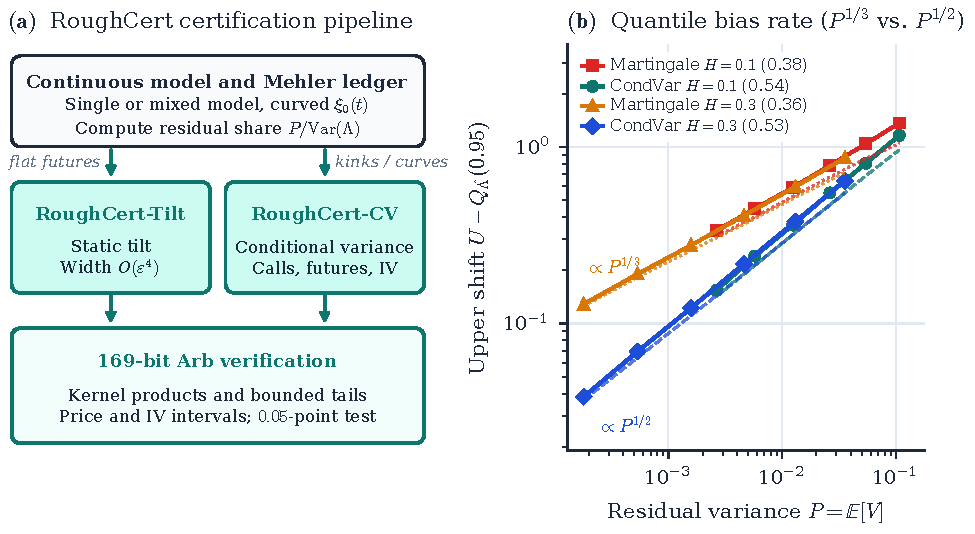
\includegraphics[width=\textwidth]{figures/fig_v3_01_pipeline_and_rates.pdf}
\caption{(a) Overview of the \RoughCert{} deterministic certification pipeline (\RoughCertTilt{} and
\RoughCertCV{}). (b) Upper quantile shift above $Q_{\hat\Lambda}(0.95)$ for $\int_0^1 B_H(s)^2\dd s$ versus
residual variance $P$ ($n=4,\dots,128$), confirming the $P^{1/3}$ versus $P^{1/2}$ local rates.}\label{fig:rates_cond}
\end{figure}
\ifTwoColumn\else\FloatBarrier\fi
%
\section{VIX futures: head-to-head \RoughCert{} audit of published benchmarks}\label{sec:vix_futures}

Under the rough Bergomi model \citep{BayerFrizGatheral2016}, the squared VIX index at maturity $T$ over
the forward window $\Delta$ is the Wick-exponential functional \eqref{eq:vix2_def}. Different articles
use two distinct kernel normalisations and window lengths:
\begin{itemize}
\item \citet{BayerFrizGatheral2016}, \citet{JacquierMartiniMuguruza2018}, and \citet{BonesiniCallegaroJacquier2023}
  write $K(u,s)=\eta_{\mathrm{P1}}\sqrt{2H}(u-s)^{H-1/2}$ (with $\Delta=30/365$ or $\Delta=1/12$);
\item \citet{BourgeyDeMarco2022} and \citet{BourgeyDeMarcoGobet2023} write $K(u,s)=a(u-s)^{H-1/2}$ with
  $\Delta=1/12$, where $a=\eta_{\mathrm{P1}}\sqrt{2H}$.
\end{itemize}
Every table below states $(H,T,\Delta,a)$ explicitly so no comparison mixes conventions. All VIX futures
prices are quoted in volatility points ($100\times\mathrm{VIX}_T$), where one standard Cboe futures tick
equals $0.05$ volatility points \citep{CBOE2024VIX}. Every enclosure in this section is \lab{Arb-certified}.

\subsection{Headline \RoughCertTilt{} audit: separating published expansions by more than one tick}\label{sec:vix_headline}
Table~\ref{tab:vix_headline} summarises our 169-bit Arb \RoughCertTilt{} verification across eight headline parameter cells
covering literature configurations and E14 base and stress tests. Every cell passes our strict outward-rounded enclosure
gate (total bracket width below $0.05$ points and Arb endpoint enclosure width at most $1.39\times10^{-3}$ points
for $L$ and $6.41\times10^{-11}$ points for $U$). Three decisive findings emerge directly from the
outward-rounded intervals:
\begin{enumerate}
\item \emph{Machine-verified $>1$ tick violation by BDG~(2023) in stress regimes.} In the six-month
  stress cell ($H=0.10$, $T=0.5$, $\eta_{\mathrm{P1}}=3.0$, $a=1.34164$, $\Delta=30/365$), the static
  \RoughCertTilt{} bracket is $[\ArbStressTiltedL,\ArbStressTiltedU]$ (width $\ArbStressTiltedW$ points), while
  our independent Arb evaluation of \citet[Theorem~2.2]{BourgeyDeMarcoGobet2023} gives $\ArbStressBDG$
  points---exceeding the continuous rough-Bergomi upper bound $U$ by at least $+\ArbStressBDGGap$ points
  ($\TickStress$ Cboe ticks; and by $+\GapStressRefined$ points, or $\TickStressRefined$ ticks, using the refined \RoughCertCV{} upper bound
  of Section~\ref{sec:vix_options}). On BDG's own Figure~1 extreme cell ($H=0.10$, $T=0.5$,
  $a=1.5$, $\Delta=1/12$), the \RoughCertTilt{} bracket is $[\ArbFigOneL,\ArbFigOneU]$ (width $\ArbFigOneW$
  points) while BDG~(2023) gives $\ArbFigOneBDG$, certifying an upward bias of at least
  $+\ArbFigOneBDGGap$ points ($\TickFigOne$ Cboe ticks). Even at ultra-rough $H=0.05$ ($\eta_{\mathrm{P1}}=3.0$,
  $T=0.5$, Table~\ref{tab:vix_e14}), the observed BDG excess reaches $+\ArbStressHZeroFiveBDGGap$ points
  ($\TickStressHZeroFive$ ticks).
\item \emph{Certified downward bias of the moment-matched lognormal proxy.} Across all eight headline
  cells, the exact moment-matched lognormal proxy $F_{\mathrm{LN}}=M_1^{3/4}M_2^{-1/8}$ lies strictly
  below our Arb lower bound $L$. Its downward bias exceeds one Cboe tick not only in stress
  ($-\ArbStressLNGap$ points in E14 stress and $-\ArbFigOneLNGap$ points at $a=1.5$, or $\TickLNStress$--$\TickLNFigOne$
  ticks), but already in moderate regimes: $-\LNGapFigSix$ points ($\TickLNFigSix$ ticks) in BDG Figure~6 ($a=1.0$,
  $T=3$\,m) and $-\LNGapBCJ$ points ($\TickLNBCJ$ ticks) in BCJ~\S5.3 ($H=0.10$, $\eta_{\mathrm{P1}}=1.9$,
  $T=6$\,m).
\item \emph{Disentangling continuum and $500$-cell grid targets in Bourgey and De Marco~(2022).}
  On the multilevel Monte Carlo benchmark of \citet[Section~3.3]{BourgeyDeMarco2022} ($H=0.10$, $T=0.5$,
  $a=0.5$, $\Delta=1/12$, published MLMC price $22.18135$), the continuous-time Arb bracket is
  $[\ArbBDContL,\ArbBDContU]$ (width $\ArbBDContW$ points), whereas the exact Arb tilted bracket for
  their $500$-cell right-rectangle discrete target $\Lambda_{500}=\frac{1}{500}\sum_{j=1}^{500}\xi_T(T+j\Delta/500)$
  (zero spatial discretisation error) is $[\ArbBDGridL,\ArbBDGridU]$ (Figure~\ref{fig:vix_bcj_disjoint}(a)).
  The two Arb intervals are strictly disjoint by at least $\ArbBDDisjointGap$ points, and the published
  MLMC value $22.18135$ sits strictly inside the $500$-cell Arb enclosure, at least $\MLMCBelowGridU$ points
  below its upper endpoint. The reported estimate is compatible with its declared grid and falls outside the continuum interval.
\end{enumerate}

\IfFileExists{tables/tab_vix_headline.tex}{\begin{table}[!htbp]\centering\scriptsize\setlength{\tabcolsep}{2.2pt}
\caption{Headline 169-bit Arb-certified \RoughCertTilt{} VIX futures brackets (volatility points) across eight literature and stress-test parameter cells, audited against BDG~(2023) and lognormal proxies.}\label{tab:vix_headline}
\begin{tabular}{@{}lrrrrccrrr@{}}\toprule
 & \multicolumn{4}{c}{Contract parameters} & \multicolumn{2}{c}{\textbf{\RoughCertTilt{}} (pts)} & \multicolumn{3}{c}{Expansion and signed gaps (pts)} \\
\cmidrule(lr){2-5}\cmidrule(lr){6-7}\cmidrule(lr){8-10}
Benchmark & $H$ & $T$ (yr) & $\Delta$ (yr) & $a$ & $[L,\,U]$ & Width & BDG$_3$ & $\mathrm{BDG}_3\!-\!U$ & $\mathrm{LN}\!-\!L$ \\\midrule
Stress (E14) & 0.10 & 0.50 & 30/365 & 1.342 & \textbf{\boldmath [15.53706,\,15.55718]} & \textbf{\boldmath 0.02011} & 15.61414 & $+$0.05696$^\star$ & $-$0.2965$^\star$ \\
BDG (2023) Fig.~1 & 0.10 & 0.50 & 1/12 & 1.500 & \textbf{\boldmath [14.05216,\,14.08195]} & \textbf{\boldmath 0.02978} & 14.16307 & $+$0.08112$^\star$ & $-$0.4304$^\star$ \\
BD (2022) \S3.3 & 0.10 & 0.50 & 1/12 & 0.500 & \textbf{\boldmath [22.17993,\,22.18038]} & \textbf{\boldmath 0.00044} & 22.18192 & $+$0.00154 & $-$0.0076 \\
BDG (2023) Fig.~6 & 0.10 & 0.25 & 1/12 & 1.000 & \textbf{\boldmath [19.90857,\,19.91515]} & \textbf{\boldmath 0.00657} & 19.93666 & $+$0.02152 & $-$0.0978$^\star$ \\
BCJ (2023) \S5.3 & 0.10 & 0.50 & 1/12 & 0.850 & \textbf{\boldmath [19.81201,\,19.81546]} & \textbf{\boldmath 0.00345} & 19.82707 & $+$0.01161 & $-$0.0581$^\star$ \\
Base ($H=0.10$) & 0.10 & 1/12 & 30/365 & 0.850 & \textbf{\boldmath [22.01885,\,22.02193]} & \textbf{\boldmath 0.00307} & 22.03265 & $+$0.01073 & $-$0.0358 \\
Base ($H=0.05$) & 0.05 & 1/12 & 30/365 & 0.601 & \textbf{\boldmath [22.50390,\,22.50644]} & \textbf{\boldmath 0.00254} & 22.51588 & $+$0.00943 & $-$0.0214 \\
Stress ($H=0.30$) & 0.30 & 0.50 & 30/365 & 2.324 & \textbf{\boldmath [12.66828,\,12.66937]} & \textbf{\boldmath 0.00108} & 12.67214 & $+$0.00278 & $-$0.0680$^\star$ \\
\midrule
BD (2022) 500-cell & 0.10 & 0.50 & 1/12 & 0.500 & \textbf{\boldmath [22.18102,\,22.18141]} & \textbf{\boldmath 0.00039} & \multicolumn{3}{c}{MLMC $= 22.18135$ (inside grid band)} \\
\bottomrule\end{tabular}
\smallskip\par\raggedright\scriptsize\emph{Notes:} Bold identifies the tilted interval and width before display rounding. $H$ is the Hurst exponent, $T$ maturity, $\Delta$ the window and $a=\eta_{\mathrm{P1}}\sqrt{2H}$. BDG$_3$ is the third-order expansion; LN is lognormal. Signed gaps use the nearest bound. $^\star$ exceeds one Cboe tick ($0.05$ pts). Endpoint enclosure widths (at most $1.4\times 10^{-3}$ pts) are included.
\end{table}
}{}

\subsection{Complete 15-cell E14 suite and JMM~(2018) lower-bound audit}\label{sec:vix_e14}
Table~\ref{tab:vix_e14} extends the audit to all $15$ cells of the base, curved-$\xi_0$
\citep[Scenario~2: $\xi_0(t)=0.234^2(1+t)^2$]{JacquierMartiniMuguruza2018}, and stress design
($\Delta=30/365$), taking the sharpest outward-rounded Arb bracket from Theorem~\ref{thm:tilted} and
Proposition~\ref{prop:arb}. Every cell resolves well below one Cboe tick: maximum width is
$\ArbEFourteenBaseMaxW$ points across the $12$ base and curved cells and $\ArbEFourteenMaxW$ points across
all $15$ cells, narrowing the published bounds of \citet[Theorem~3.3]{JacquierMartiniMuguruza2018} by
factors of $\ArbJMMRatioLo\times$ to $\ArbJMMRatioHi\times$. To credit the strength of JMM~(2018) fairly,
Table~\ref{tab:vix_e14} also reports $U-L_{\mathrm{JMM}}$, the worst-case error of JMM's lower bound
alone: JMM's lower bound is accurate to within $0.008$--$0.105$ points in base and curved cells (reaching
$0.146$--$0.152$ points for the $H=0.05,0.10$ stress cells), while the massive width ratio reflects JMM's variance-swap
upper bound $\sqrt{\E[\mathrm{VIX}_T^2]}$. Our Arb bounds sharpen both sides simultaneously without a
reference simulation, with timings reported separately in the archive.

\IfFileExists{tables/tab_vix_e14_15cells.tex}{\begin{table}[!htbp]\centering\scriptsize\setlength{\tabcolsep}{3.6pt}
\caption{Complete 15-cell Arb-certified \RoughCert{} VIX futures suite (volatility points, $\Delta=30/365$), benchmarked against JMM~(2018), BDG~(2023), and lognormal proxies.}\label{tab:vix_e14}
\begin{tabular}{@{}rlcrrrrrr@{}}\toprule
 & & \multicolumn{2}{c}{\textbf{\RoughCert{}} (pts)} & \multicolumn{3}{c}{JMM (2018) bounds} & \multicolumn{2}{c}{Certified proxy gap (pts)} \\
\cmidrule(lr){3-4}\cmidrule(lr){5-7}\cmidrule(lr){8-9}
$H$ & $T$ & $[L,\,U]$ & Width & \shortstack{Width\\(pts)} & \shortstack{Lower-bound\\error limit (pts)} & \shortstack{Width\\ratio} & $\mathrm{BDG}_3-U$ & $\mathrm{LN}-L$ \\\midrule
\multicolumn{9}{@{}l}{\emph{Panel A: Base regime ($\eta_{\mathrm{P1}}=1.9$, flat $\xi_0=0.235^2$)}} \\
\addlinespace[1.5pt]
0.05 & 1w & \textbf{\boldmath [23.12106,\,23.12218]} & \textbf{\boldmath 0.00111} & 0.427 & 0.0491 & 385$\times$ & $+$0.00667 & $-$0.0078 \\
0.05 & 1m & \textbf{\boldmath [22.50405,\,22.50644]} & \textbf{\boldmath 0.00238} & 1.056 & 0.0622 & 443$\times$ & $+$0.00943 & $-$0.0216 \\
0.05 & 3m & \textbf{\boldmath [21.77897,\,21.78174]} & \textbf{\boldmath 0.00277} & 1.783 & 0.0641 & 645$\times$ & $+$0.01015 & $-$0.0306 \\
0.10 & 1w & \textbf{\boldmath [22.96234,\,22.96354]} & \textbf{\boldmath 0.00119} & 0.589 & 0.0516 & 494$\times$ & $+$0.00708 & $-$0.0121 \\
0.10 & 1m & \textbf{\boldmath [22.01917,\,22.02193]} & \textbf{\boldmath 0.00275} & 1.546 & 0.0675 & 563$\times$ & $+$0.01073 & $-$0.0361 \\
0.10 & 3m & \textbf{\boldmath [20.83240,\,20.83583]} & \textbf{\boldmath 0.00343} & 2.734 & 0.0698 & 799$\times$ & $+$0.01165 & $-$0.0525$^\star$ \\
0.30 & 1w & \textbf{\boldmath [23.06690,\,23.06697]} & \textbf{\boldmath 0.00006} & 0.442 & 0.0084 & 7,679$\times$ & $+$0.00022 & $-$0.0016 \\
0.30 & 1m & \textbf{\boldmath [22.01988,\,22.02002]} & \textbf{\boldmath 0.00014} & 1.493 & 0.0126 & 11,449$\times$ & $+$0.00048 & $-$0.0070 \\
0.30 & 3m & \textbf{\boldmath [20.20115,\,20.20133]} & \textbf{\boldmath 0.00017} & 3.313 & 0.0138 & 19,586$\times$ & $+$0.00060 & $-$0.0129 \\
\midrule
\multicolumn{9}{@{}l}{\emph{Panel B: Curved forward variance ($\eta_{\mathrm{P1}}=1.9$, JMM Scenario~2: $\xi_0(t)=0.234^2(1+t)^2$)}} \\
\addlinespace[1.5pt]
0.05 & 1m & \textbf{\boldmath [25.21964,\,25.22259]} & \textbf{\boldmath 0.00294} & 1.190 & 0.0948 & 405$\times$ & --- & --- \\
0.10 & 1m & \textbf{\boldmath [24.68133,\,24.68480]} & \textbf{\boldmath 0.00346} & 1.737 & 0.1042 & 502$\times$ & --- & --- \\
0.30 & 1m & \textbf{\boldmath [24.66989,\,24.67087]} & \textbf{\boldmath 0.00098} & 1.682 & 0.0346 & 1,731$\times$ & --- & --- \\
\midrule
\multicolumn{9}{@{}l}{\emph{Panel C: Stress regime ($\eta_{\mathrm{P1}}=3.0$, $T=6$\,m, flat $\xi_0=0.235^2$)}} \\
\addlinespace[1.5pt]
0.05 & 6m & \textbf{\boldmath [18.26959,\,18.28359]} & \textbf{\boldmath 0.01399} & 5.363 & 0.1463 & 383$\times$ & $+$0.05525$^\star$ & $-$0.1920$^\star$ \\
0.10 & 6m & \textbf{\boldmath [15.54052,\,15.55650]} & \textbf{\boldmath 0.01598} & 8.096 & 0.1516 & 506$\times$ & $+$0.05764$^\star$ & $-$0.3000$^\star$ \\
0.30 & 6m & \textbf{\boldmath [12.66836,\,12.66937]} & \textbf{\boldmath 0.00101} & 10.860 & 0.0293 & 10,852$\times$ & $+$0.00278 & $-$0.0680$^\star$ \\
\bottomrule\end{tabular}
\smallskip\par\raggedright\scriptsize\emph{Notes:} Bold identifies the narrowest available \RoughCert{} interval and its width. $H$ is the Hurst exponent and $T$ maturity. The JMM error limit is $U-L_{\rm JMM}$; the ratio divides JMM width by \RoughCert{} width. BDG$_3$ is the third-order expansion; LN is lognormal. $^\star$ exceeds one Cboe tick ($0.05$ pts). A dash marks an unevaluated proxy.
\end{table}
}{}

\subsection{Parameter-space phase boundaries (BDG Figs.~1--2) and BCJ~(2023) multi-curve term structures}\label{sec:vix_sweeps}
Figure~\ref{fig:vix_phase_boundary} shows certified separations at the sampled parameters of BDG~(2023) and
the lognormal proxy across the two flagship parameter sweeps of \citet[Figures~1--2]{BourgeyDeMarcoGobet2023}
($T=0.5$, $\Delta=1/12$, $\xi_0=0.235^2$). Along the vol-of-vol sweep at $H=0.10$
(Figure~\ref{fig:vix_phase_boundary}(a)), the Arb tilted width, the observed BDG excess
$\mathrm{BDG}_3-U$, and the lognormal shortfall $L-\mathrm{LN}$ grow with $a$ (the width law is given by
Theorem~\ref{thm:tilted}(iii)), staying strictly ordered: the lognormal shortfall first exceeds the $0.05$-point Cboe tick on the sampled grid at $a=1.00$, following a sub-tick shortfall at $a=0.80$, whereas the lower bound on BDG's error lies below one tick at $a\approx1.20$ ($\mathrm{BDG}_3-U=\SweepAOneTwo$) and enters the Arb-certified $>1$-tick
violation zone at the sampled values $a=1.35,1.50$ ($+\SweepAOneThreeFive$ at $a=1.35$, $+\SweepAOneFive$ at $a=1.50$). Along the roughness sweep at $a=1.0$ (Figure~\ref{fig:vix_phase_boundary}(b)), decreasing $H$ from $0.40$
to $0.05$ amplifies both kernel dispersion and competitor biases sharply: at $H=0.05$ ($a=1.0$, $T=6$\,m),
even this moderate vol-of-vol drives BDG~(2023) above our Arb upper bound by at least $\SweepHBDG$ points
($\SweepHBDGTicks$ ticks) and the lognormal proxy below our Arb lower bound by at least $\SweepHLN$ points
($\SweepHLNTicks$ ticks), while our Arb width stays below $\SweepHWidth$ points (marginally above half a tick
at $H=0.05$, and below $\SweepHWidthRest$ points for $H\ge0.10$).

\begin{figure}[!htbp]\centering
\IfFileExists{figures/fig_v3_02_phase_boundaries.pdf}{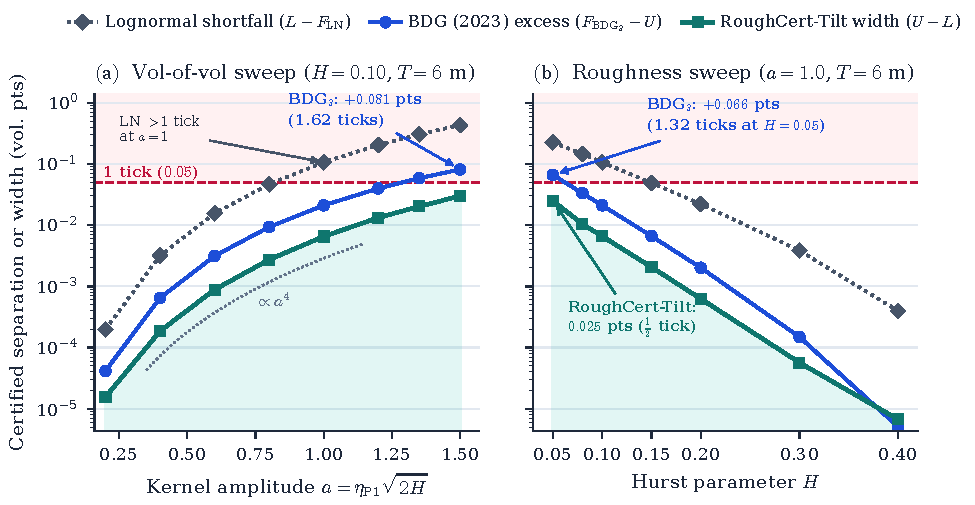
\includegraphics[width=\textwidth]{figures/fig_v3_02_phase_boundaries.pdf}}{\fbox{fig\_v3\_02 pending}}
\caption{Arb-certified bias of BDG~(2023) ($F_{\mathrm{BDG}_3}-U$) and lognormal proxy ($L-F_{\mathrm{LN}}$)
versus \RoughCertTilt{} width ($U-L$) at $T=6$\,m. (a) Vol-of-vol $a$ sweep ($H=0.10$); (b) Hurst $H$ sweep
($a=1.0$). Shaded region exceeds one Cboe tick ($0.05$ pts).}\label{fig:vix_phase_boundary}
\end{figure}

To benchmark against the functional quantisation suite of \citet[Section~5.3]{BonesiniCallegaroJacquier2023}
($H=0.10$, $\eta_{\mathrm{P1}}=1.9$, $\Delta=1/12$), we evaluate all $18$ combinations of their three
forward-variance curves ($\xi_0(t)=0.234^2\{1,(1+t)^2,\sqrt{1+t}\}$) and six maturities
($T\in\{1,2,3,6,9,12\}$ months; Figure~\ref{fig:vix_bcj_disjoint}(b) and Supplementary Table~S1).
Because the unweighted barycentre $h_0$ keeps the exact Pfaff ${}_2F_1$ inner products across arbitrary
curves, \RoughCertCV{} (Proposition~\ref{prop:arb}(c)--(d)) certifies every continuous-time future to width
at most $\ArbBCJMaxW$ points ($\ArbBCJRatioLo\times$--$\ArbBCJRatioHi\times$ narrower than JMM~2018),
while the 960-path BCJ quantiser sits visibly below all three term structures.

\begin{figure}[!htbp]\centering
\IfFileExists{figures/fig_v3_03_disjoint_and_curves.pdf}{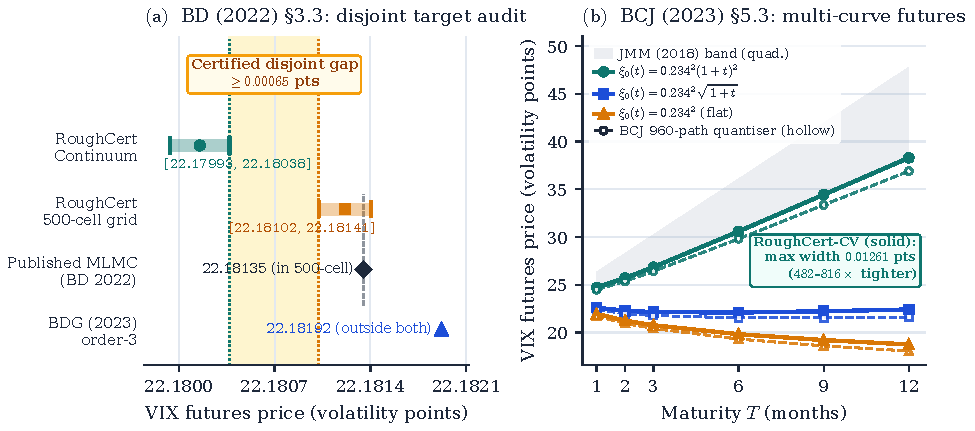
\includegraphics[width=\textwidth]{figures/fig_v3_03_disjoint_and_curves.pdf}}{\fbox{fig\_v3\_03 pending}}
\caption{(a) Disjoint 169-bit \RoughCertTilt{} enclosures for the continuum and $500$-cell grid in
\citet[Section~3.3]{BourgeyDeMarco2022}, isolating the published MLMC value ($22.18135$) inside the grid
target. (b) \RoughCertCV{} futures term structures versus BCJ~(2023) 960-path quantisers and JMM~(2018)
bounds.}\label{fig:vix_bcj_disjoint}
\end{figure}

\subsection{Extension to mixed rough Bergomi futures}\label{sec:mixed_rbergomi}
In mixed rough Bergomi the forward variance is a $\lambda$-weighted mixture of Wick exponentials with distinct
vol-of-vol levels, so no single exponential tilt reproduces its law. Conditioning on the shared Gaussian factor
$Z=W(h_0)/\norm{h_0}$ in Proposition~\ref{prop:arb}(c)--(d) instead retains the full nonlinear mixture inside
$X(z)$ while keeping the residual covariance $D_0$ tiny. Table~\ref{tab:vix_mixed} reports five mixed rough Bergomi cells ($H=0.10$, $\Delta=1/12$,
$\xi_0=0.235^2$): Scenario~1 $(a_1,a_2,\lambda)=(1.4,0.7,0.3)$ at $T\in\{1,3,6\}$ months and a higher
vol-of-vol stress mixture $(1.6,0.7,0.4)$ at $T\in\{3,6\}$ months. Across Scenario~1, the Arb brackets
achieve widths of at most $\ArbMixScenMaxW$ points ($<1/8$ of one Cboe tick), while BDG's order-three
mixed expansion, evaluated by floating-point quadrature, exceeds the respective upper endpoints by
approximately $+\MixScenGapLo$ to $+\MixScenGapHi$ points; under the stress mixture, the
observed BDG excess widens to $+\ArbMixMaxBDGGap$ points while our Arb width stays below
$\ArbMixAllMaxW$ points.

\IfFileExists{tables/tab_vix_mixed.tex}{\begin{table}[!htbp]\centering\footnotesize\setlength{\tabcolsep}{4.0pt}
\caption{Mixed rough Bergomi VIX futures (volatility points, $H=0.10$, $\Delta=1/12$, $\xi_0=0.235^2$): \RoughCertCV{} enclosures versus BDG~(2023) mixed weak expansions.}\label{tab:vix_mixed}
\begin{tabular}{@{}lcrccrrrr@{}}\toprule
 & & & \multicolumn{2}{c}{\textbf{\RoughCertCV{}} (pts)} & \multicolumn{3}{c}{BDG (2023) mixed (pts)} & \\
\cmidrule(lr){4-5}\cmidrule(lr){6-8}
Regime & $(a_1,a_2,\lambda)$ & $T$ & $[L,\,U]$ & Width & BDG$_0$ & BDG$_3$ & $\mathrm{BDG}_3-U$ & \shortstack{Setup / solve\\(s)} \\\midrule
Scenario~1 & (1.4,\,0.7,\,0.3) & 1m & \textbf{\boldmath [21.86821,\,21.87169]} & \textbf{\boldmath 0.00347} & 21.70815 & 21.88995 & $+$0.01826 & 1.8 / 5.2 \\
Scenario~1 & (1.4,\,0.7,\,0.3) & 3m & \textbf{\boldmath [20.63299,\,20.63780]} & \textbf{\boldmath 0.00481} & 20.47861 & 20.65502 & $+$0.01722 & 1.6 / 5.2 \\
Scenario~1 & (1.4,\,0.7,\,0.3) & 6m & \textbf{\boldmath [19.69027,\,19.69553]} & \textbf{\boldmath 0.00525} & 19.54665 & 19.71098 & $+$0.01546 & 1.5 / 5.0 \\
Stress & (1.6,\,0.7,\,0.4) & 3m & \textbf{\boldmath [19.85257,\,19.85950]} & \textbf{\boldmath 0.00692} & 19.65869 & 19.88916 & $+$0.02966 & 1.6 / 5.0 \\
Stress & (1.6,\,0.7,\,0.4) & 6m & \textbf{\boldmath [18.75046,\,18.75762]} & \textbf{\boldmath 0.00716} & 18.57762 & 18.78286 & $+$0.02523 & 1.4 / 4.8 \\
\bottomrule\end{tabular}
\smallskip\par\raggedright\scriptsize\emph{Notes:} Bold identifies the conditional-variance interval and width. $a_1,a_2$ are factor loadings, $\lambda$ is the mixing weight and $T$ is maturity in months. BDG$_0$ and BDG$_3$ denote zeroth- and third-order floating-point expansions. The signed gap compares the third-order value with the certified upper bound.
\end{table}
}{}
\ifTwoColumn\else\FloatBarrier\fi
%
\section{VIX options and implied-volatility smiles}\label{sec:vix_options}

VIX futures are smooth concave functions of $\mathrm{VIX}_T^2$, so the static \RoughCertTilt{} bracket of
Theorem~\ref{thm:tilted} already attains sub-tick precision. VIX calls and puts introduce a payoff kink
at the strike $K$, degrading the single-tilt Lipschitz control \eqref{eq:tilted_opt_lip} from
$O(\varepsilon^4)$ to $O(\varepsilon^2)$. This section applies the 169-bit Arb \RoughCertCV{} engine of
Proposition~\ref{prop:arb}(c)--(e) to five published option and smile benchmarks, contrasting its precision
against \eqref{eq:tilted_opt_lip}, the order-three weak expansion of \citet{BourgeyDeMarcoGobet2023}, the
direct IV expansion of \citet{LiaoAgarwalBourgey2026}, the moment-matched lognormal proxy, and the multilevel
Monte Carlo benchmark of \citet{BourgeyDeMarco2022}. Every call, put, and Black-76 implied-volatility bracket
below carries the label \lab{Arb-certified} and propagates forward-price uncertainty rigorously via
Proposition~\ref{prop:arb}(e).

\subsection{Pure rough Bergomi: BDG Figure~6, LAB (2026), and stress smiles}\label{sec:pure_smiles}
We first audit the three-month VIX smile of \citet[Figure~6]{BourgeyDeMarcoGobet2023} ($H=0.10$,
$T=0.25$, $a=1.0$, $\Delta=1/12$, $\xi_0=0.235^2$) across nine log-moneyness strikes
$k=\log(K/F_{\mathrm{mid}})\in[-0.4,0.4]$ (Table~\ref{tab:vix_smiles}, top panel; Figure~\ref{fig:vix_smiles},
left). The comparisons use common physical strikes.
\begin{enumerate}
\item \emph{Conditional variance tightens the option control.} The static Lipschitz
  control \eqref{eq:tilted_opt_lip} gives a uniform option error bound of $\LipFigSix$ volatility points,
  whereas the Arb conditional-variance call brackets have widths $\FigSixCallWLo$--$\FigSixCallWHi$ volatility points
  (ratios of approximately $\LipRatioLo$--$\LipRatioHi$ against that bound), tightening smoothly into the out-of-the-money right wing.
\item \emph{Forward inflation induces systematic downward IV bias in BDG~(2023).} Although BDG's
  order-three call prices lie inside our Arb call brackets at six of nine strikes (falling outside by
  $+\SepKmFour$ at $k=-0.40$, $+\SepKmThree$ at $k=-0.30$, and $-\SepKpFour$ at $k=+0.40$), inverting those calls
  against BDG's own inflated order-three forward ($19.9367$ versus our Arb future $[19.9092,19.9152]$)
  shifts the BDG implied-volatility curve downward by $\FigSixIVGapLo$--$\FigSixIVGapHi$ percentage points
  below our Arb IV lower bound at \emph{all nine strikes} ($\BDGIVPureLo\%$--$\BDGIVPureHi\%$ versus $[113.48\%,114.05\%]$ to
  $[114.83\%,115.01\%]$).
\item \emph{Machine-verified positive VIX skew and lognormal failure.} Because the Arb IV upper bound at
  $k=-0.40$ ($114.05\%$) lies strictly below the Arb IV lower bound at $k=+0.40$ ($114.83\%$), the
  continuous rough-Bergomi VIX smile is machine-verified to be higher at the right endpoint by at least $\PureSkew$
  percentage points across $[-0.4,0.4]$. By contrast, the moment-matched lognormal proxy predicts a flat
  smile inside $[\LNIVPureLo\%,\LNIVPureHi\%]$, exceeding the Arb IV upper bound by
  $\LNAbovePureLo$--$\LNAbovePureHi$ percentage points at every strike.
\end{enumerate}

A flat-variance scaling check inspired by \citet{LiaoAgarwalBourgey2026} rescales the forward-variance
level ($\xi_0=0.24^2$, $H=0.10$, $a=1.0$, $T=0.25$, $\Delta=1/12$, seven strikes $k\in[-0.3,0.3]$). Flat scaling
of $\xi_0$ leaves Black-76 implied volatilities invariant ($[113.66\%,114.13\%]$ at $k=-0.30$ rising to
$[114.66\%,114.86\%]$ at $k=+0.30$, with all call widths $\ScaleCallWLo$--$\ScaleCallWHi$ volatility points and
forward $[20.3328,20.3390]$), while BDG order-three IV remains $\ScaleIVGapLo$--$\ScaleIVGapHi$ percentage points below the
Arb lower bound at every sampled strike.

Under the six-month stress parameters ($H=0.10$, $T=0.5$, $\eta_{\mathrm{P1}}=3.0$, $a=1.34164$,
$\Delta=30/365$, Table~\ref{tab:vix_smiles}, Panel~B; Figure~\ref{fig:vix_smiles}(b)), the divergence
widens substantially. On our refined spatial--Gaussian grid ($M=320$, $N_z=620$; improving the initial
$200\times 420$ ATM IV width from $\StressATMOld$ to $\StressATMNew$ percentage points), \RoughCertCV{} narrows the futures
bracket to $[15.54225,15.55578]$ (width at most $\StressFutW$ points, lifting the certified BDG$_3$ futures
excess to at least $+\GapStressRefined$ points, or $\TickStressRefined$ Cboe ticks) and delivers call widths of $\StressCallWLo$--$\StressCallWHi$ points across
$K/F\in[0.70,2.00]$ (versus $\LipStress$ points from \eqref{eq:tilted_opt_lip}). BDG order-three calls exceed
the \RoughCertCV{} upper bound at five of six strikes (by $+\StressExcWing$ at $K/F=0.70$ and $+\StressExcATM$ at the
money), while both BDG order-three IV ($\BDGIVStressLo\%$--$\BDGIVStressHi\%$) and the direct IV expansion of
\citet{LiaoAgarwalBourgey2026} ($\LABIVStressLo\%$--$\LABIVStressHi\%$) fall below the lower edge at all six
strikes by $\StressIVGapLo$--$\StressIVGapHi$ percentage points. The continuum IV bands at the first and last strikes are $[126.58\%,127.44\%]$ and $[127.77\%,128.06\%]$.
The lognormal proxy, flat inside $[\LNIVStressLo\%,\LNIVStressHi\%]$, exceeds the IV upper edge by
$\LNAboveStressLo$--$\LNAboveStressHi$ percentage points.

\subsection{Continuum versus 500-cell grid ATM call: Bourgey and De Marco (2022)}\label{sec:bd2022_call}
On the multilevel Monte Carlo benchmark of \citet[Section~3.3]{BourgeyDeMarco2022} ($H=0.10$, $T=0.5$,
$a=0.5$, $\Delta=1/12$, $\xi_0=0.235^2$, strike $K=22.18135$, published ATM call $2.98840$), we evaluate
both the continuous-time \RoughCertCV{} call bracket and the exact $500$-cell right-rectangle
\RoughCertCV{} call bracket (zero spatial discretisation error). The continuous-time futures interval is $[22.17970,\,22.18063]$ and the grid interval is $[22.18090,\,22.18174]$, with widths at most $0.00092$ and $0.00084$ points. The published futures estimate lies inside the grid interval, whereas the order-three value $22.18192$ exceeds both upper bounds.
For the call, the continuum interval is $[2.98837,\,2.99007]$ and the grid interval is $[2.98798,\,2.98953]$, with widths at most $0.00170$ and $0.00155$ points. Both contain the published estimate $2.98840$ and the order-three value $2.98844$. At fixed strike $K$, the small upward shift in the right-rectangle forward partially
offsets its slight reduction in forward-window variance on the call payoff, so the call brackets overlap
at this moderate vol-of-vol ($a=0.5$).

\subsection{Mixed rough Bergomi: certifying a steep upward-sloping VIX smile}\label{sec:mixed_smile}
The pure-model example above gives a modest end-to-end IV increase. Earlier empirical studies document difficulties reproducing market VIX skews
\citep{HorvathJacquierTankov2020,Romer2022}. The mixed rough Bergomi model
$\xi_T(u)=\xi_0(u)[\lambda\cE(a_1\phi_u)+(1-\lambda)\cE(a_2\phi_u)]$ \citep{Bergomi2016,BourgeyDeMarcoGobet2023}
produces a steep upward-sloping VIX smile, and Proposition~\ref{prop:arb}(c)--(e) certifies it
directly without simulation by conditioning on the shared Gaussian direction $Z=W(h_0)/\norm{h_0}$.

Table~\ref{tab:vix_smiles} (bottom panel) and Figure~\ref{fig:vix_smiles} (right) report the three-month
mixed rough Bergomi smile ($H=0.10$, $T=0.25$, $\Delta=1/12$, $\xi_0=0.235^2$, $a_1=1.4$, $a_2=0.7$,
$\lambda=0.3$) across $k\in[-0.3,0.3]$. Across all seven strikes, the Arb call brackets achieve widths
$\MixCallWLo$--$\MixCallWHi$ volatility points and establish strictly increasing Black-76 implied volatility across the seven sampled strikes, rising from $[92.95\%,93.33\%]$ at $k=-0.30$ to $[99.55\%,99.73\%]$ at $k=+0.30$ (a certified
positive skew of at least $+\MixSkew$ percentage points, with IV bracket widths of only
$\MixIVWLo$--$\MixIVWHi$ percentage points). The root-split calculation in Section~\ref{sec:methods_vtwo} distinguishes the weak expansion from its Gauss--Hermite implementation.

\IfFileExists{tables/tab_vix_smiles.tex}{\begin{table}[!htbp]\centering\footnotesize\setlength{\tabcolsep}{2.5pt}
\caption{\RoughCertCV{} Arb-certified VIX call prices (pts) and Black-76 implied volatilities (\%) versus BDG~(2023), LAB~(2026), and lognormal proxies across three smile regimes.}\label{tab:vix_smiles}
\begin{tabular}{@{}rrccrrccrr@{}}\toprule
 & & \multicolumn{4}{c}{VIX call price (pts)} & \multicolumn{4}{c}{Black-76 implied volatility (\%)} \\
\cmidrule(lr){3-6}\cmidrule(lr){7-10}
\shortstack{Log\\moneyness} & \shortstack{Strike\\(pts)} & \textbf{\RoughCertCV{}} & Width & BDG$_3$ & LN & \textbf{\RoughCertCV{}} & BDG$_3$ & LAB & LN \\\midrule
\multicolumn{10}{@{}l}{\emph{Panel A: Pure rough Bergomi --- BDG~(2023) Fig.~6 ($H=0.10$, $T=3$\,m, $a=1.0$, $\Delta=1/12$, $\xi_0=0.235^2$)}} \\
\addlinespace[1.5pt]
$-$0.40 & 13.347 & \textbf{\boldmath [7.84856,\,7.85733]} & \textbf{\boldmath 0.00877} & 7.85998 & 7.84470 & \textbf{\boldmath [113.48,\,114.05]} & 113.21 & --- & 116.88 \\
$-$0.20 & 16.303 & \textbf{\boldmath [6.10446,\,6.11242]} & \textbf{\boldmath 0.00796} & 6.11170 & 6.12630 & \textbf{\boldmath [113.84,\,114.23]} & 113.58 & --- & 116.88 \\
$+$0.00 & 19.912 & \textbf{\boldmath [4.47632,\,4.48298]} & \textbf{\boldmath 0.00666} & 4.47993 & 4.51522 & \textbf{\boldmath [114.18,\,114.46]} & 113.93 & --- & 116.88 \\
$+$0.20 & 24.320 & \textbf{\boldmath [3.07248,\,3.07769]} & \textbf{\boldmath 0.00521} & 3.07340 & 3.11666 & \textbf{\boldmath [114.51,\,114.72]} & 114.28 & --- & 116.88 \\
$+$0.40 & 29.705 & \textbf{\boldmath [1.96166,\,1.96577]} & \textbf{\boldmath 0.00410} & 1.96102 & 2.00067 & \textbf{\boldmath [114.83,\,115.01]} & 114.62 & --- & 116.88 \\
\midrule
\multicolumn{10}{@{}l}{\emph{Panel B: Stress regime (refined grid) --- E14 ($H=0.10$, $T=6$\,m, $\eta_{\mathrm{P1}}=3.0$, $\Delta=30/365$, $\xi_0=0.235^2$)}} \\
\addlinespace[1.5pt]
$-$0.36 & 10.883 & \textbf{\boldmath [7.23501,\,7.25033]} & \textbf{\boldmath 0.01532} & 7.26835 & 7.13723$^\star$ & \textbf{\boldmath [126.58,\,127.44]} & 126.14 & 126.18 & 131.61 \\
$-$0.16 & 13.215 & \textbf{\boldmath [6.22615,\,6.24021]} & \textbf{\boldmath 0.01406} & 6.25308 & 6.16585$^\star$ & \textbf{\boldmath [126.82,\,127.50]} & 126.38 & 126.40 & 131.61 \\
$+$0.00 & 15.547 & \textbf{\boldmath [5.39485,\,5.40761]} & \textbf{\boldmath 0.01276} & 5.41662 & 5.36336 & \textbf{\boldmath [127.02,\,127.58]} & 126.58 & 126.58 & 131.61 \\
$+$0.22 & 19.434 & \textbf{\boldmath [4.30816,\,4.31895]} & \textbf{\boldmath 0.01079} & 4.32353 & 4.30982 & \textbf{\boldmath [127.27,\,127.71]} & 126.84 & 126.84 & 131.61 \\
$+$0.41 & 23.321 & \textbf{\boldmath [3.49377,\,3.50292]} & \textbf{\boldmath 0.00914} & 3.50469 & 3.51549 & \textbf{\boldmath [127.46,\,127.84]} & 127.05 & 127.04 & 131.61 \\
$+$0.69 & 31.095 & \textbf{\boldmath [2.38736,\,2.39413]} & \textbf{\boldmath 0.00677} & 2.39285 & 2.42679 & \textbf{\boldmath [127.77,\,128.06]} & 127.38 & 127.37 & 131.61 \\
\midrule
\multicolumn{10}{@{}l}{\emph{Panel C: Mixed rough Bergomi --- Scenario~1 ($H=0.10$, $T=3$\,m, $a_1=1.4$, $a_2=0.7$, $\lambda=0.3$, $\Delta=1/12$)}} \\
\addlinespace[1.5pt]
$-$0.30 & 15.287 & \textbf{\boldmath [6.62323,\,6.63029]} & \textbf{\boldmath 0.00706} & 6.63570 & --- & \textbf{\boldmath [92.95,\,93.33]} & 92.90 & --- & --- \\
$-$0.20 & 16.895 & \textbf{\boldmath [5.66039,\,5.66732]} & \textbf{\boldmath 0.00692} & 5.67089 & --- & \textbf{\boldmath [93.94,\,94.25]} & 93.87 & --- & --- \\
$+$0.00 & 20.636 & \textbf{\boldmath [3.91767,\,3.92367]} & \textbf{\boldmath 0.00600} & 3.92401 & --- & \textbf{\boldmath [96.06,\,96.28]} & 95.96 & --- & --- \\
$+$0.10 & 22.806 & \textbf{\boldmath [3.17187,\,3.17741]} & \textbf{\boldmath 0.00553} & 3.17647 & --- & \textbf{\boldmath [97.18,\,97.38]} & 97.08 & --- & --- \\
$+$0.30 & 27.855 & \textbf{\boldmath [1.97201,\,1.97679]} & \textbf{\boldmath 0.00477} & 1.97408 & --- & \textbf{\boldmath [99.55,\,99.73]} & 99.45 & --- & --- \\
\bottomrule\end{tabular}
\smallskip\par\raggedright\scriptsize\emph{Notes:} Log moneyness is $\log(K/F_{\rm mid})$. Bold gives certified prices, widths and implied volatilities. BDG$_3$ is the third-order expansion, LAB the direct implied-volatility expansion and LN the lognormal proxy. Dashes mark unavailable comparisons. $^\star$ denotes price separation exceeding one Cboe tick ($0.05$ pts). Panel C uses exercise-boundary splitting.
\end{table}
}{}

\begin{figure}[!htbp]\centering
\IfFileExists{figures/fig_v3_04_vix_smiles.pdf}{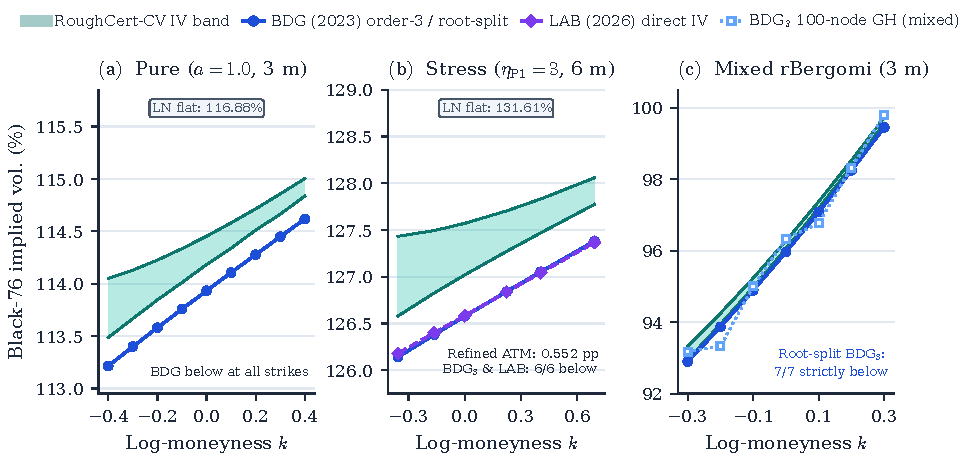
\includegraphics[width=\textwidth]{figures/fig_v3_04_vix_smiles.pdf}}{\fbox{fig\_v3\_04 pending}}
\caption{\RoughCertCV{} Black-76 implied-volatility bands versus BDG~(2023), LAB~(2026), and lognormal
proxies. (a) Pure rBergomi ($a=1.0$, $3$\,m); (b) refined stress cell ($\eta_{\mathrm{P1}}=3$, $6$\,m);
(c) mixed rBergomi ($3$\,m, root-split versus the authors' $100$-node implementation).}\label{fig:vix_smiles}
\end{figure}
\ifTwoColumn\else\FloatBarrier\fi
%
\section{Comparing expansions, factor reductions, and quantisers}\label{sec:methods_vtwo}
A deterministic \RoughCert{} enclosure supports two decisions. For a method value enclosed in $[A,B]$ and a
continuous-model bracket $[L,U]$, the signed pricing error lies in $[A-U,B-L]$. The method is certified
tick-accurate when that interval fits inside $[-0.05,0.05]$, and certified biased when it lies strictly on
one side of zero, which is the disjointness used throughout this section; calls use the same $0.05$-point
price tolerance, and implied-volatility differences are measured in percentage points.

\subsection{The exercise boundary and direct implied volatility}\label{sec:direct_expansion}
In the mixed expansion of \citet[Theorem~3.1]{BourgeyDeMarcoGobet2023}, let
$y_j(z)=\bar\xi\,\lambda_j\exp(\mu_j+s_jz)$ and $Y(z)=y_1(z)+y_2(z)$, where
$\bar\xi=\Delta^{-1}\int_T^{T+\Delta}\xi_0(u)\dd u$. For a fixed strike $K>0$, $Y(z)=K^2$ has a unique root
for positive amplitudes. The weak derivative of the call under a shift in component $j$ is
$y_j(z)\mathbf{1}_{\{Y(z)>K^2\}}/(2\sqrt{Y(z)})$. Integrating against the normal density times
$\gamma_{1,j}+\gamma_{2,j}z/s_j+\gamma_{3,j}(z^2-1)/s_j^2$ and adding the proxy call evaluates the
published coefficient expression rigorously (the exercise boundary has zero normal mass; the original mixed
theorem states its remainder for smooth payoffs).

At $k=-0.20$, the authors' implementation---$100$-node Gauss--Hermite quadrature with $10^{-4}$
finite-difference derivatives---yields $93.326\%$, whereas splitting
the integral at exercise in Arb gives $[93.8671,93.8672]\%$ against a \RoughCertCV{} band of
$[93.9407,94.2487]\%$. At $k=+0.10$ the corresponding values are $96.768\%$, $[97.0817,97.0818]\%$, and
$[97.1870,97.3764]\%$. All seven root-split IVs fall strictly below the lower edge, with edge separations of $\MixSplitSepLo$ to
$\MixSplitSepHi$ percentage points, while that $100$-node implementation adds a separate strike-dependent
kink oscillation (Figure~\ref{fig:methoderrors}(a)).

For a single kernel, equation~(21) of \citet{LiaoAgarwalBourgey2026} gives the direct IV formula
\[
 \widehat\sigma(K)=\frac{v}{2}+\frac{\gamma_2}{2vT}+\frac{3\gamma_3}{8vT}
                 -\frac{\gamma_3\log(S/K)}{v^3T^2},
 \qquad v=\frac{\norm{h_0^{(a)}}}{\sqrt{T}},
\]
where $S$ is the zeroth-order VIX forward and $h_0^{(a)}$ is the barycentre with amplitude $a$. Fixing
physical strikes via the order-three forward on the authors' $\Delta=30/365$ window and enclosing both
the direct formula and the continuous model in 169-bit Arb establishes a downward IV bias at all $30$
strikes for $H=0.10$, at $22$ of $30$ strikes for $H=0.23$, and at all $6$ stress strikes
(Table~\ref{tab:competitors}, Panel~A; the remaining eight comparisons overlap, with zero strikes above).

\begin{figure}[!htbp]\centering
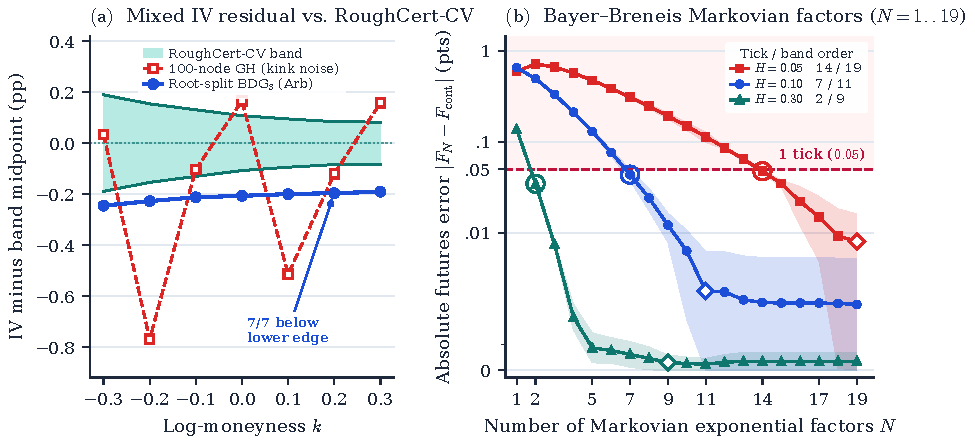
\includegraphics[width=\textwidth]{figures/fig_v3_05_mixed_and_markov.pdf}
\caption{(a) Mixed-smile IV deviations from the continuum midpoint. (b) Absolute futures-error enclosures and midpoints for $N=1,\ldots,19$. Circles mark one-tick accuracy and diamonds mark containment in the fixed continuum band.}\label{fig:methoderrors}
\end{figure}

\subsection{Markovian factor count and product quantisation}\label{sec:factor_counts}
We evaluate the geometric Gaussian rule and numerical $L^2$ kernel optimisation of
\citet{BayerBreneis2023}, freezing the returned positive nodes and weights at their recorded decimal values.
For $K_N(t)=\sum_j w_j e^{-\gamma_j t}$, the finite model has exact covariance
\[
 C_N(x,y)=\sum_{i,j} w_i w_j e^{-\gamma_i x-\gamma_j y}\,\frac{1-e^{-(\gamma_i+\gamma_j)T}}{\gamma_i+\gamma_j},
\]
with the quotient read as $T$ when $\gamma_i+\gamma_j=0$, enabling verified \RoughCertCV{} enclosures of every $N$-factor model. On the flat
three-month contract ($a=1$, $\Delta=1/12$, $\xi_0=0.235^2$), the Arb-proved minimum optimised factor counts
achieving $<0.05$-point futures error are $14$, $7$, and $2$ for $H=0.05$, $0.10$, and $0.30$
(Figure~\ref{fig:methoderrors}(b); Table~\ref{tab:competitors}, Panel~B), with every smaller integer proved
outside. For full containment inside the fixed continuum band ($M=144$, $N_z=320$), the proved minimum
orders are $19$, $11$, and $9$ (with every smaller integer proved disjoint from that fixed band). At $H=0.05$, conditioning the
tilted residual on the contrast $k_{\Delta/14}-k_\Delta$ cleanly separates the $13$-factor error
$[-0.0671,-0.0611]$ from the $14$-factor error $[-0.0496,-0.0453]$. On the three fixed-strike calls
($K\in\{18,22,26\}$), all minimum orders are exact at $H=0.10$ and $0.30$, while at $H=0.05$ two strikes
leave a one-factor overlap bracket ($N\in\{5,6\}$ at $K=18$ and $N\in\{1,2\}$ at $K=22$, noted explicitly in
Table~\ref{tab:competitors}). These thresholds apply to the recorded fitting horizon $T+\Delta$, nodes, and
weights rather than all possible positive exponential sums.

The functional quantiser of \citet[Remark~4.9]{BonesiniCallegaroJacquier2023} expands the Brownian input in
cosines on $[0,T+\Delta]$ while retaining continuous Gaussian variance compensation. Using their Table~1
allocations at budgets $100$ and $1000$ (and declared allocations $(6,4,2)$ and $(10,4,3,2,2)$ at $50$ and
$500$), we enclose both scalar normal centroids and delivery integrals in Arb. Even at $960$ product paths,
all $18$ literature futures prices are underestimated by at least $0.208$ points on $\Delta=1/12$ (and by
$0.209$--$1.412$ points on $\Delta=30/365$; Table~\ref{tab:competitors}, Panel~C; Figure~\ref{fig:scoreboard}(b)).
A separate forward-field Karhunen--Lo\`eve diagnostic in the archive assesses basis choice across two
delivery grids.

\begin{table}[!htbp]\centering\scriptsize\setlength{\tabcolsep}{3.3pt}
\caption{Multi-method competitor audit against \RoughCertCV{} across direct IV expansions (LAB~2026), Markovian factor reductions (Bayer--Breneis), and product functional quantisation (BCJ~2023).}\label{tab:competitors}
\begin{tabular}{@{}lcccccc@{}}\toprule
\multicolumn{7}{@{}l}{\emph{Panel A: Direct implied-volatility expansion \citep[Eq.~(21)]{LiaoAgarwalBourgey2026} against \textbf{\RoughCertCV{}}}} \\
\addlinespace[1.5pt]
 & & & \multicolumn{3}{c}{Comparison with \textbf{\RoughCertCV{}}} & \\
\cmidrule(lr){4-6}
Regime & $H$ & Maturity & Strikes below & \shortstack{Strikes\\overlapping} & \shortstack{Max shortfall\\(pp)} & Verdict \\\midrule
LAB author grid & 0.10 & 1\,m & 10/10 & 0/10 & 0.487 & All below \\
LAB author grid & 0.10 & 3\,m & 10/10 & 0/10 & 0.236 & All below \\
LAB author grid & 0.10 & 6\,m & 10/10 & 0/10 & 0.140 & All below \\
LAB author grid & 0.23 & 1\,m & 10/10 & 0/10 & 0.021 & All below \\
LAB author grid & 0.23 & 3\,m & 8/10 & 2/10 & 0.008 & 2 overlap \\
LAB author grid & 0.23 & 6\,m & 4/10 & 6/10 & 0.002 & 6 overlap \\
Stress ($\eta_{\mathrm{P1}}=3$) & 0.10 & 6\,m & 6/6 & 0/6 & 0.435 & All below \\
\midrule
\multicolumn{7}{@{}l}{\emph{Panel B: Bayer--Breneis Markovian factor thresholds ($T=3$\,m, $a=1.0$, $\Delta=1/12$, $\xi_0=0.235^2$)}} \\
\addlinespace[1.5pt]
Hurst $H$ & \shortstack{Futures\\within tick} & \shortstack{Futures inside\\reference band} & Call $K=18$ & Call $K=22$ & Call $K=26$ & Verification \\\midrule
0.05 & 14 & 19 & 5 or 6$^\dagger$ & 1 or 2$^\dagger$ & 1 & Exact except $^\dagger$ \\
0.10 & 7 & 11 & 2 & 1 & 5 & All exact minima \\
0.30 & 2 & 9 & 1 & 2 & 2 & All exact minima \\
\midrule
\multicolumn{7}{@{}l}{\emph{Panel C: BCJ~(2023) product functional quantisation signed futures errors (pts) and median runtimes (s)}} \\
\addlinespace[1.5pt]
Budget / Paths & \multicolumn{2}{c}{18-cell ($\Delta=1/12$)} & 18-cell ($30/365$) & Stress (pts) & Setup (s) & Price (s) \\\midrule
50 / 48 & \multicolumn{2}{c}{[$-$2.077,\,$-$0.321]$^\star$} & [$-$2.092,\,$-$0.322]$^\star$ & [$-$1.239,\,$-$1.219]$^\star$ & 0.12 & 0.07 \\
100 / 96 & \multicolumn{2}{c}{[$-$1.851,\,$-$0.280]$^\star$} & [$-$1.863,\,$-$0.282]$^\star$ & [$-$1.184,\,$-$1.164]$^\star$ & 0.12 & 0.14 \\
500 / 480 & \multicolumn{2}{c}{[$-$1.450,\,$-$0.216]$^\star$} & [$-$1.458,\,$-$0.216]$^\star$ & [$-$0.994,\,$-$0.972]$^\star$ & 0.14 & 0.71 \\
1000 / 960 & \multicolumn{2}{c}{[$-$1.406,\,$-$0.208]$^\star$} & [$-$1.412,\,$-$0.209]$^\star$ & [$-$0.965,\,$-$0.942]$^\star$ & 0.17 & 1.42 \\
\bottomrule\end{tabular}
\smallskip\par\raggedright\scriptsize\emph{Notes:} Panel A counts implied-volatility intervals against the bold reference method; pp means percentage points. Panel B gives minimum factor counts. $^\dagger$ marks unresolved adjacent counts. Panel C gives quantiser minus continuum futures by window and budget. $^\star$ marks an entire error range beyond one Cboe tick ($0.05$ pts).
\end{table}
%

\subsection{Common curved contract scoreboard and numerical refinements}\label{sec:curved_score}
Table~\ref{tab:common} and Figure~\ref{fig:scoreboard}(a) compare all eight methods on a single curved
forward-variance contract ($H=0.10$, $T=3$\,m, $\Delta=1/12$, $a=1.9\sqrt{2H}$, $\xi_0(t)=0.234^2(1+t)^2$,
strike $K=27$). The $12$-factor futures, call and IV enclosures each overlap the continuum band.
The $500$-cell forward lies $0.00098$--$0.00999$ points above it. The lognormal future is more than one
tick low, while its IV is $1.26$--$1.76$ percentage points high. The $960$-path BCJ future is
$0.425$--$0.438$ points low and its IV is $5.51$--$5.86$ percentage points low. The BDG and LAB
curved-kernel IV enclosures both overlap the continuum interval. Their numerical point evaluations,
$96.821\%$ and $96.827\%$, lie approximately $0.14$ and $0.13$ percentage points below its lower edge;
the certified comparisons leave the sign unresolved.

\begin{figure}[!htbp]\centering
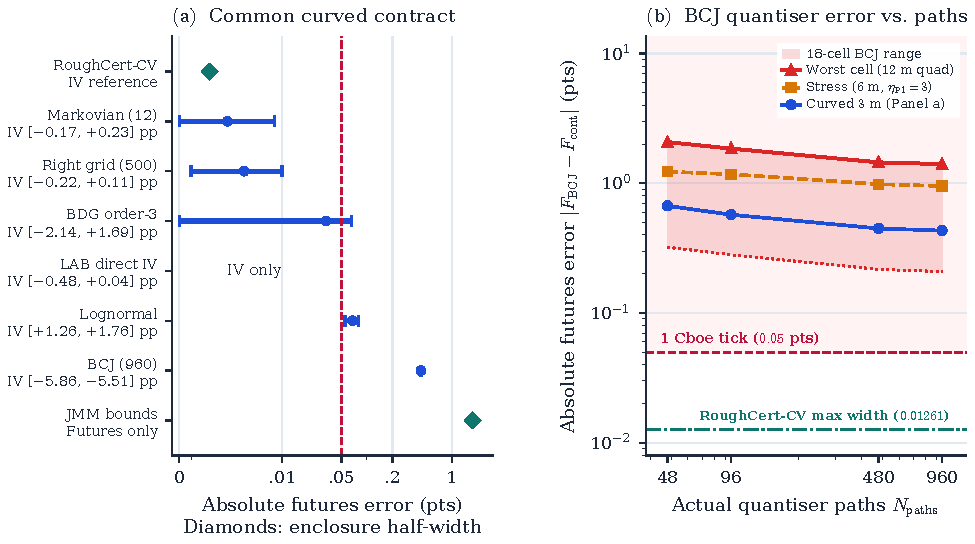
\includegraphics[width=\textwidth]{figures/fig_v3_06_scoreboard_and_quantizer.pdf}
\caption{(a) Curved contract at $K=27$. Bars enclose absolute futures errors, diamonds indicate enclosure half-widths, and row labels give signed IV differences from the continuum in percentage points. (b) BCJ quantisation error across four budgets and the largest 18-cell \RoughCertCV{} width.}\label{fig:scoreboard}
\end{figure}

\begin{table}[!htbp]\centering\scriptsize\setlength{\tabcolsep}{3.4pt}
\caption{Eight-method comparison on a common curved forward-variance contract ($H=0.10$, $T=3$\,m, $\Delta=1/12$, $\xi_0(t)=0.234^2(1+t)^2$, strike $K=27$ pts).}\label{tab:common}
\begin{tabular}{@{}lccccr@{}}\toprule
 & & \multicolumn{3}{c}{Outward-rounded enclosures at the same strike} & \\
\cmidrule(lr){3-5}
Method & Engine & Futures (pts) & Call (pts) & Black-76 IV (\%) & Against reference \\\midrule
\textbf{\RoughCertCV{} (continuum)} & Arb & \textbf{\boldmath [26.8389,\,26.8441]} & \textbf{\boldmath [5.078,\,5.085]} & \textbf{\boldmath [96.95,\,97.14]} & Reference \\
Markovian ($N=12$) & Arb & [26.8359,\,26.8417] & [5.077,\,5.086] & [96.97,\,97.19] & Overlaps on all three \\
500-cell right grid & Arb & [26.8450,\,26.8489] & [5.079,\,5.085] & [96.92,\,97.07] & Future above \\
BDG (2023) order-3 & Arb & [26.8125,\,26.9046] & [5.012,\,5.148] & [95.00,\,98.64] & Overlaps on all three \\
LAB (2026) direct IV & Arb & --- & --- & [96.66,\,96.99] & IV overlaps \\
Moment-matched lognormal & Arb & [26.7636,\,26.7838]$^\star$ & [5.082,\,5.159] & [98.40,\,98.72] & Future below; IV above \\
BCJ quantiser (960 paths) & Arb & [26.4061,\,26.4132]$^\star$ & [4.532,\,4.538]$^\star$ & [91.28,\,91.45] & Below on all three \\
JMM (2018) bounds & Arb & [26.7216,\,30.2303] & --- & --- & Contains futures band \\
\bottomrule\end{tabular}
\smallskip\par\raggedright\scriptsize\emph{Notes:} Bold identifies the continuous-time reference. Arb encloses each stated model or approximation. Each implied volatility (IV) uses its own forward at $K=27$. A dash marks an unavailable output. $^\star$ denotes a futures or call separation exceeding $0.05$ pts, the standard futures tick used for comparison.
\end{table}
%

Finally, two targeted refinements sharpen the stress regime. First, optimising the scalar tilt
$h=0.98646905\,h_0$ in \RoughCertTilt{} cuts the flat stress futures width from $0.01968$ to $0.01447$ points
on the same $320$-cell grid (and from $0.03003$ to $0.02092$ points at $a=1.5$ with $h=0.98331070\,h_0$),
improving both endpoints rigorously. Second, refining the \RoughCertCV{} stress smile mesh from $200\times 420$
to $320\times 620$ reduces the ATM IV width from $\StressATMOld$ to $\StressATMNew$ percentage points
(Table~\ref{tab:vix_smiles}, Panel~B). Two independent simulation diagnostics---a Brownian-kernel SVD
control-variate QMC check ($12$ scrambled Sobol nets per design, at $48$ delivery nodes with $2^{14}$ points and $96$ delivery
nodes with $2^{17}$ points) and a $130$-decimal-digit Cholesky
sampler at $40$ delivery nodes---place all \SimChecks/\SimChecks\ forward, call, and IV estimates inside the
corresponding \RoughCert{} intervals.
\ifTwoColumn\else\FloatBarrier\fi
%
\section{Variance risk and integrated variance: when certificates stay wide}\label{sec:variance_risk}

The sub-tick VIX bounds of Sections~\ref{sec:vix_futures}--\ref{sec:vix_options} raise a natural question:
does the same framework produce equally tight bounds for realised-variance derivatives under rough
volatility? Examining two spot-variance functionals---integrated variance in the tractable rough
Stein--Stein model and integrated variance in rough Bergomi---demonstrates that the answer is no, and
shows how the exact residual share $P_\mu/\Var(\Lambda_\mu)$ diagnoses the contrast before any simulation.

\subsection{Rough Stein--Stein variance risk against an exact characteristic-function law}\label{sec:case_steinstein}
Here the conditional-variance principle behind \RoughCertCV{} supplies statistical risk brackets. Their sampling uncertainty is distinct from the deterministic Arb pricing enclosures. In the rough Stein--Stein model, spot volatility is Gaussian, $\sigma_t=\sigma_0+\nu W_t^H$ with $W^H$
Riemann--Liouville fractional Brownian motion, and the characteristic function of integrated variance
$\Lambda=\int_0^T\sigma_t^2\dd t$ is known in closed form \citep{AbiJaber2022}. Because $\Lambda$ is a
quadratic subordinated functional, both the conditional-expectation monitor $\hat\Lambda=\E[\Lambda\mid\mathcal{G}]$
and the conditional variance $V=\Var(\Lambda\mid\mathcal{G})$ given $n$ monitoring dates are explicit
quadratic forms in the whitened observations,
$\hat\Lambda=d_0+\ell^\top\xi+\xi^\top A\xi$ and $V=c_0+b^\top\xi+\xi^\top\Omega\xi$, computed once by
graded quadrature. We test one month of daily closes ($T=1/12$, $n=21$, $\sigma_0=0.2$, $\nu=0.1$,
$H\in\{0.05,0.10,0.30\}$) on the $99\%$ quantile (value at risk of a short variance swap) and calls
$\E(\Lambda-k)_+$ at $k=\E\Lambda$ and $k=\E\Lambda+2\,\mathrm{sd}$ ($50$ replications of $K=2\times10^5$
daily paths, DKW level $a=0.01$, \lab{statistical}$(0.99)$). An independent Karhunen--Lo\`eve expansion
($2{,}500$ nodes, Fourier inversion) provides the reference law, matching the exact mean to $10^{-9}$ and
the ledger variance to within \EthirteenKLvar\% (omitted tail share $5.8\times10^{-6}$ at $H=0.05$).

Table~\ref{tab:e13} shows that daily monitoring leaves substantial continuum bias: the exact RMS error of
the daily Riemann sum is \EthirteenRiLo--\EthirteenRiHi\% of $\mathrm{sd}(\Lambda)$, biasing standard
daily Monte Carlo by \EthirteenNaiveLo\ to \EthirteenNaiveHi\ standard deviations on the $99\%$ quantile
and by \EthirteenPriceBiasLo\% to \EthirteenPriceBiasHi\% on calls. Every certified bracket attained
empirical coverage \EthirteenCovMin. Conditioning on daily closes with conditional variance and exact
binomial order statistics (Proposition~\ref{prop:condvar}(ii)) shrank the $99\%$ VaR brackets to
\EthirteendLo--\EthirteendHi\ standard deviations (sampling floor \EthirteendFloorHi), and computing
$\E(\hat\Lambda-k)_+$ from its quadratic-form characteristic function shrank ATM call brackets to
\EthirteencAtmLo--\EthirteencAtmHi\% of the exact price.

For $H\le0.10$, daily closes alone still leave $\ResShareDailyLo$--$\ResShareDailyHi\%$ of $\Var(\Lambda)$
unexplained. Simulating
intraday volatility paths conditionally on the daily closes via an exact Gaussian bridge leaves the
continuum law of $\Lambda$ unchanged while refining $\mathcal{G}$ (Table~\ref{tab:e13}, Panel~C): moving from one
to \EthirteenbMaxDaya\ points per day reduces the residual share from \EthirteenbSaOne\% to
\EthirteenbSaEight\% ($H=0.05$) and from \EthirteenbSbOne\% to \EthirteenbSbEight\% ($H=0.10$), cutting
the estimated conditional Cantelli $99\%$ bracket width from approximately \EthirteenbDaOne\ to \EthirteenbDaEight\ standard
deviations ($H=0.05$) and from \EthirteenbDbOne\ to \EthirteenbDbEight\ ($H=0.10$) while preserving
$1.00$ coverage. Thus the ledger quantifies the reduction in the residual variance from each tested monitoring refinement before
pricing a portfolio.

\begin{table}[!htbp]\centering\scriptsize\setlength{\tabcolsep}{3.5pt}
\caption{Rough Stein--Stein one-month integrated variance ($n=21$ daily closes): statistical $99\%$ VaR brackets (in exact sd), variance-call widths (relative to exact price), and intraday Gaussian-bridge refinement.}\label{tab:e13}
\begin{tabular}{@{}rrrcccccr@{}}\toprule
\multicolumn{9}{@{}l}{\emph{Panel A: Daily-close $99\%$ VaR bracket widths in exact sd (empirical coverage in parentheses)}} \\
\addlinespace[1.5pt]
 & \multicolumn{2}{c}{RMS error (\% of sd)} & \multicolumn{2}{c}{Baseline width (sd)} & \multicolumn{3}{c}{\textbf{\RoughCertCV{}} and sampling (sd)} & \\
\cmidrule(lr){2-3}\cmidrule(lr){4-5}\cmidrule(lr){6-8}
$H$ & Daily sum & Monitor & Riemann $W_2$ & Martingale & Cantelli & DKW floor & \shortstack{Binomial width\\and floor} & \shortstack{Daily bias\\(sd)} \\\midrule
0.05 & 42.7\% & 37.0\% & 8.50 (1.00) & 5.39 (1.00) & \textbf{\boldmath 3.45} (1.00) & 0.38 & \textbf{\boldmath 2.61} (1.00)/0.06 & $+$0.315 \\
0.10 & 25.0\% & 23.0\% & 5.70 (1.00) & 3.72 (1.00) & \textbf{\boldmath 1.99} (1.00) & 0.41 & \textbf{\boldmath 1.45} (1.00)/0.07 & $+$0.165 \\
0.30 & 7.7\% & 6.5\% & 2.54 (1.00) & 1.59 (1.00) & \textbf{\boldmath 0.71} (1.00) & 0.39 & \textbf{\boldmath 0.37} (1.00)/0.06 & $+$0.093 \\
\midrule
\multicolumn{9}{@{}l}{\emph{Panel B: Variance calls $\E(\Lambda-k)_+$ --- certified width / exact price (coverage in parentheses)}} \\
\addlinespace[1.5pt]
$H$ & Strike $k$ & Exact price & Lipschitz & Convex & Scarf--Lo & \shortstack{Exact\\monitor law} & & \shortstack{Daily bias\\(\%)} \\\midrule
0.05 & $\E\Lambda$ & $4.7\times 10^{-4}$ & 2.74 (1.00) & 1.04 (1.00) & \textbf{\boldmath 0.751} (1.00) & \textbf{\boldmath 0.177} (1.00) & & $+$11.1\% \\
0.05 & $+2\,\mathrm{sd}$ & $2.3\times 10^{-5}$ & 55.10 (1.00) & 20.67 (1.00) & \textbf{\boldmath 12.923} (1.00) & \textbf{\boldmath 1.702} (1.00) & & $+$61.0\% \\
0.10 & $\E\Lambda$ & $5.2\times 10^{-4}$ & 1.78 (1.00) & 0.80 (1.00) & \textbf{\boldmath 0.589} (1.00) & \textbf{\boldmath 0.083} (1.00) & & $+$6.0\% \\
0.10 & $+2\,\mathrm{sd}$ & $2.8\times 10^{-5}$ & 32.97 (1.00) & 14.60 (1.00) & \textbf{\boldmath 9.900} (1.00) & \textbf{\boldmath 0.756} (1.00) & & $+$28.6\% \\
0.30 & $\E\Lambda$ & $3.8\times 10^{-4}$ & 1.01 (1.00) & 0.71 (1.00) & \textbf{\boldmath 0.632} (1.00) & \textbf{\boldmath 0.011} (1.00) & & $+$3.7\% \\
0.30 & $+2\,\mathrm{sd}$ & $1.7\times 10^{-5}$ & 21.82 (1.00) & 15.04 (1.00) & \textbf{\boldmath 13.366} (1.00) & \textbf{\boldmath 0.123} (1.00) & & $+$17.5\% \\
\midrule
\multicolumn{9}{@{}l}{\emph{Panel C: Intraday Gaussian-bridge conditioning refinement for $99\%$ VaR (widths in continuum sd)}} \\
\addlinespace[1.5pt]
$H$ & \shortstack{Observations\\per day} & \shortstack{Residual\\share} & & Martingale & Cantelli & DKW floor & & \shortstack{Cantelli\\coverage} \\\midrule
0.05 & 1 & $1.4\times 10^{-1}$ & & 5.39 & \textbf{\boldmath 3.46} & 0.38 & & 1.00 \\
0.05 & 2 & $7.1\times 10^{-2}$ & & 4.12 & \textbf{\boldmath 2.30} & 0.39 & & 1.00 \\
0.05 & 4 & $3.5\times 10^{-2}$ & & 3.16 & \textbf{\boldmath 1.59} & 0.41 & & 1.00 \\
0.05 & 8 & $1.7\times 10^{-2}$ & & 2.46 & \textbf{\boldmath 1.15} & 0.40 & & 1.00 \\
0.10 & 1 & $5.3\times 10^{-2}$ & & 3.72 & \textbf{\boldmath 1.99} & 0.42 & & 1.00 \\
0.10 & 2 & $2.4\times 10^{-2}$ & & 2.82 & \textbf{\boldmath 1.38} & 0.42 & & 1.00 \\
0.10 & 4 & $1.1\times 10^{-2}$ & & 2.18 & \textbf{\boldmath 1.02} & 0.42 & & 1.00 \\
0.10 & 8 & $4.8\times 10^{-3}$ & & 1.73 & \textbf{\boldmath 0.80} & 0.43 & & 1.00 \\
\bottomrule\end{tabular}
\smallskip\par\raggedright\scriptsize\emph{Notes:} Bold identifies conditional-variance widths, rounded up. Parentheses give empirical coverage. The monitor is conditional expectation; sd is the continuum standard deviation. DKW denotes the Dvoretzky--Kiefer--Wolfowitz sampling floor. The binomial cell gives width (coverage) / floor. Daily bias compares the daily estimate with the reference law. Panels A/B use 50 replications and C uses 10.
\end{table}
%

\subsection{Rough Bergomi integrated variance: the structural contrast with VIX}\label{sec:case_iv}
For one-month integrated variance $\mathrm{IV}=\int_0^{1/12} v_t\dd t$ and integrated volatility
$\mathrm{IVol}=\int_0^{1/12}\sqrt{v_t}\dd t$ under rough Bergomi ($\xi_0=0.235^2$, $\eta_{\mathrm{P1}}=1.9$,
$H\in\{0.05,0.10,0.30\}$), the spot variance path is integrated directly rather than smoothed by a forward
expectation. Conditioning on the $n=21$ daily closes requires a singularity-corrected per-sample rule for
$V(\xi)=\iint\hat X_s\hat X_u(e^{\eta^2 D(s,u)}-1)\dd s\dd u$ (maximum relative per-sample audit difference
\EsixcAudit, added conservatively to $v$; \lab{statistical}$(0.99)$ over $K=2\times10^5$ paths).

Table~\ref{tab:e6c} summarises the outcome. Although conditional variance narrows the $99\%$ quantile
brackets by factors \EsixcRatio\ over martingale-sharp bounds and the conditional Scarf--Lo bound narrows
variance-call brackets by factors \EsixcPriceGainLo--\EsixcPriceGainHi\ over convex-order bounds (with
fine-grid Monte Carlo diagnostics lying inside \EsixcInside/\EsixcCells\ quantile brackets and
\EsixcPriceIn/\EsixcPriceN\ call brackets), the absolute widths remain $\EsixcWidthLo$--$\EsixcWidthHi$ standard deviations
on daily-close quantiles. The separate 256-date quantile widths appear in Table~\ref{tab:e6c}, Panel~A. These brackets serve as model
validation envelopes, not quoting intervals.

The exact residual share explains why rough Bergomi produces both the narrowest and the widest brackets in
this study. On the VIX forward window $[T,T+\Delta]$, every forward variance $\xi_T(u)$ averages the same
past Brownian history on $[0,T]$ through a kernel smooth across the diagonal, so a single Gaussian
direction leaves at most $\ShareVIXBase\%$ of $\Var(\mathrm{VIX}_T^2)$ in base regimes ($\ShareVIXStress\%$
in six-month $\eta_{\mathrm{P1}}=3$ stress). On spot integrated variance $\int_0^T v_t\dd t$, by contrast, fresh rough
innovations arrive at every instant $t\in[0,T]$, so even $21$ daily closes leave up to $\ShareIVHi\%$ of
$\Var(\mathrm{IV})$ unexplained at $H=0.05$. Roughness alone therefore does not determine certifiability;
the computable residual share $P_\mu/\Var(\Lambda_\mu)$ separates tractable low-rank functionals from
path-dominated ones before any simulation is launched.

\begin{table}[!htbp]\centering\footnotesize\setlength{\tabcolsep}{2.7pt}
\caption{Rough Bergomi one-month integrated variance and volatility from $21$ daily closes: statistical $99\%$ quantile widths (in sd) and median variance-call bounds ($\times 10^4$).}\label{tab:e6c}
\begin{tabular}{@{}llrcccccc@{}}\toprule
\multicolumn{9}{@{}l}{\emph{Panel A: $99\%$ quantile widths in exact sd ($21$ daily closes vs.\ $256$-date refinement)}} \\
\addlinespace[1.5pt]
 & & & \multicolumn{4}{c}{21-date quantile widths (sd) and ratio} & \multicolumn{2}{c}{Diagnostics} \\
\cmidrule(lr){4-7}\cmidrule(lr){8-9}
Functional & $H$ & \shortstack{Monitor RMS\\(\% of sd)} & Martingale & \textbf{Cantelli} & DKW floor & \shortstack{Width\\ratio} & \shortstack{256 dates\\(sd)} & \shortstack{Monte Carlo\\in band} \\\midrule
Integrated variance & 0.05 & 44\% & 7.38 & \textbf{\boldmath 6.00} & 0.88 & 1.23$\times$ & 3.96 & 1.00 \\
Integrated volatility & 0.05 & 38\% & 5.91 & \textbf{\boldmath 4.16} & 0.54 & 1.42$\times$ & 2.65 & 1.00 \\
Integrated variance & 0.10 & 30\% & 6.12 & \textbf{\boldmath 4.60} & 1.12 & 1.33$\times$ & 3.16 & 1.00 \\
Integrated volatility & 0.10 & 24\% & 4.36 & \textbf{\boldmath 2.72} & 0.62 & 1.60$\times$ & 1.99 & 1.00 \\
Integrated variance & 0.30 & 7\% & 2.64 & \textbf{\boldmath 1.65} & 0.96 & 1.60$\times$ & 1.42 & 1.00 \\
Integrated volatility & 0.30 & 7\% & 1.93 & \textbf{\boldmath 0.98} & 0.56 & 1.98$\times$ & 0.89 & 1.00 \\
\midrule
\multicolumn{9}{@{}l}{\emph{Panel B: Variance-call brackets ($\times 10^4$) vs.\ fine-grid Monte Carlo diagnostic}} \\
\addlinespace[1.5pt]
$H$ & Strike & & \multicolumn{2}{c}{Convex order} & \multicolumn{2}{c}{\textbf{Conditional Scarf--Lo}} & \shortstack{Fine-grid\\estimate} & \\\midrule
0.05 & $\E\,\mathrm{IV}$ &  & \multicolumn{2}{c}{[10.362,\,22.828]} & \multicolumn{2}{c}{\bfseries\boldmath [10.362,\,17.512]} & 12.265 &  \\
0.05 & $+2\,\mathrm{sd}$ &  & \multicolumn{2}{c}{[0.859,\,13.037]} & \multicolumn{2}{c}{\bfseries\boldmath [0.859,\,6.729]} & 2.064 &  \\
0.10 & $\E\,\mathrm{IV}$ &  & \multicolumn{2}{c}{[11.898,\,23.209]} & \multicolumn{2}{c}{\bfseries\boldmath [11.898,\,18.427]} & 13.552 &  \\
0.10 & $+2\,\mathrm{sd}$ &  & \multicolumn{2}{c}{[1.319,\,12.335]} & \multicolumn{2}{c}{\bfseries\boldmath [1.319,\,7.068]} & 2.494 &  \\
0.30 & $\E\,\mathrm{IV}$ &  & \multicolumn{2}{c}{[9.107,\,14.147]} & \multicolumn{2}{c}{\bfseries\boldmath [9.107,\,13.256]} & 9.824 &  \\
0.30 & $+2\,\mathrm{sd}$ &  & \multicolumn{2}{c}{[0.925,\,5.755]} & \multicolumn{2}{c}{\bfseries\boldmath [0.925,\,4.822]} & 1.415 &  \\
\bottomrule\end{tabular}
\smallskip\par\raggedright\scriptsize\emph{Notes:} Bold identifies \RoughCertCV{} conditional Cantelli or Scarf--Lo results. Monitor RMS is root-mean-square error relative to the continuum standard deviation. The width ratio divides martingale by Cantelli width. DKW is the Dvoretzky--Kiefer--Wolfowitz sampling floor. Monte Carlo in band is the fraction of five replications enclosing the fine-grid diagnostic ($200{,}000$ samples per replication).
\end{table}
%
\ifTwoColumn\else\FloatBarrier\fi
%
\section{Scope, limitations, and conclusions}\label{sec:scope}

\subsection{When a continuum certificate decides a pricing or risk question}
Rough volatility produces both the sharpest and the widest brackets in this study. The exact joint error
ledger of Theorem~\ref{thm:master} identifies the reason before any derivative is priced: the
computable residual variance share $P_\mu/\Var(\Lambda_\mu)$ measures how much continuum randomness is
left unexplained by the retained Gaussian coordinates. For $\mathrm{VIX}_T^2$, every forward variance $\xi_T(u)$
integrates the same past Brownian history on $[0,T]$ through a Volterra kernel analytic across the
diagonal $u=v$, so a single Gaussian direction leaves under $\ShareVIXBase\%$ of $\Var(\mathrm{VIX}_T^2)$ in
standard rough-Bergomi regimes ($\ShareVIXStress\%$ under six-month $\eta_{\mathrm{P1}}=3$ stress). Paired with
Theorem~\ref{thm:tilted} or Proposition~\ref{prop:root} and 169-bit Arb ball arithmetic
(Proposition~\ref{prop:arb}), that low residual share delivers machine-verified futures, option, and
implied-volatility brackets in their corresponding units: the widest of the $61$ certified VIX futures
brackets reported here is $\MaxFutW$ points, below one Cboe tick. For spot integrated variance
$\int_0^T v_t\dd t$ in the same model, fresh rough innovations arrive throughout $[0,T]$, leaving up to
$\ShareIVHi\%$ of variance unexplained by daily closes; the resulting brackets serve as rigorous validation
envelopes rather than quoting tools.

This yields a concrete workflow for volatility desks and model validators:
\begin{enumerate}
\item Compute the residual variance share $P_\mu/\Var(\Lambda_\mu)$ for the target contract and
  proposed Gaussian conditioning space.
\item For VIX futures and options (single or mixed rough Bergomi, flat or curved $\xi_0$), evaluate
  \RoughCertTilt{} (Theorem~\ref{thm:tilted}) or \RoughCertCV{} (Proposition~\ref{prop:arb}). Use fast
  closed-form expansions (such as \citealp{BourgeyDeMarcoGobet2023}, \citealp{LiaoAgarwalBourgey2026}, or
  moment-matched lognormal proxies) inside calibration loops only at parameter cells where
  \RoughCert{} has certified their bias to lie below the desk's tick or implied-volatility tolerance; switch to
  the certified one-factor solver or a verified Markovian factor count wherever the certificate flags a
  violation.
\item When auditing a published Monte Carlo or multilevel benchmark, verify both the continuum target
  and the exact discrete-grid target to separate sampling error from forward-window discretisation bias.
\end{enumerate}

\subsection{Methodological boundaries and honest caveats}
Four boundaries delimit the scope of the present results:
\begin{itemize}
\item \emph{Epistemic distinction between Arb-certified and audited-quadrature results.} Every VIX
  futures, call, put, and Black-76 implied-volatility interval in Sections~\ref{sec:vix_futures}--\ref{sec:vix_options}
  encloses its stated target in the archived data, with zero uncertified
  Gaussian tail truncation and explicit outward rounding. By contrast, the paired quadratic quantile
  benchmarks (Section~\ref{sec:validation}) and the spot integrated-variance studies
  (Section~\ref{sec:variance_risk}) carry \lab{exact-identity+quadrature} and \lab{statistical}$(1-a)$
  labels whose underlying kernel integrals use graded Gauss--Legendre refinement checks rather than
  interval arithmetic.
\item \emph{Separation of asymptotic regimes.} The $O(P^{1/2})$ rate of Proposition~\ref{prop:condvar}(iii)
  describes conditional-variance quantile widths in the local density regime; the $O(\varepsilon^4)$ rate
  of Theorem~\ref{thm:tilted}(iii) describes the relative futures width in the forward-kernel dispersion
  $\varepsilon$; and the $O(\varepsilon^2)$ option bound \eqref{eq:tilted_opt_lip} explains why VIX
  options require conditional variance rather than a static tilt. None of these asymptotic rates replaces
  finite-parameter Arb verification.
\item \emph{Single-driver scope.} All theorems here concern subordinated functionals of one Gaussian
  driver (including mixed rough Bergomi with a shared Brownian motion). Joint SPX--VIX derivatives driven
  by two correlated Brownian motions $(W^{(1)},W^{(2)})$ involve both integrated variance and stochastic
  integrals $\int_0^T\sqrt{v_s}\dd W_s^{(1)}$ and require a separate two-field conditional Monte Carlo
  framework.
\item \emph{Model prices versus market calibration.} All numerical benchmarks evaluate declared
  rough-volatility models at published literature parameters; separating model-pricing error from
  market-calibration misfit requires external market-data inputs beyond the scope of this study.
\end{itemize}

\subsection{Conclusions}
We have introduced \RoughCert{}, an exact Gaussian error calculus and machine-verified certification
framework linking continuum functional approximation to deterministic derivative bounds and conditional risk
certificates. Combining the reconciled Mehler error ledger (Theorem~\ref{thm:master}), conditional-variance
square-root bounds (Proposition~\ref{prop:root}), the static \RoughCertTilt{} Girsanov--H\"older theorem with
sharp $O(\varepsilon^4)$ dispersion width (Theorem~\ref{thm:tilted}), and outward-rounded 169-bit Arb
certification via Pfaff ${}_2F_1$ inner products and Minkowski $L^2$ perturbation bounds
(\RoughCertCV{}, Proposition~\ref{prop:arb}) yields sampling-free continuous-time enclosures narrower than
one Cboe tick across pure, curved-$\xi_0$, and mixed rough Bergomi regimes. Head-to-head audits against
2022--2026 benchmarks machine-verify where order-three weak expansions exceed one full exchange tick on
futures and induce systematic downward implied-volatility bias, quantify direct implied-volatility shortfalls at $52$ of the $60$
published LAB strikes, establish minimum Markovian factor counts for the recorded fits, certify the sign of
the functional-quantiser bias, disentangle
continuum prices from $500$-cell right-rectangle multilevel Monte Carlo targets, and certify steep
upward-sloping VIX smiles in mixed rough Bergomi without simulation.
%
\ifTwoColumn\FloatBarrier\fi
\section*{CRediT authorship contribution statement}
\textbf{Eslam Ahmed:} Writing -- original draft, Visualization, Software, Methodology, Data curation, Conceptualization.
\textbf{Mohamed A. El-Beltagy:} Supervision, Conceptualization, Methodology, Validation, Data curation, Writing -- review \& editing.
\textbf{Ahmed Etman:} Writing -- review \& editing, Validation, Software, Formal analysis, Data curation.
\textbf{Sroor M. Elnady:} Writing -- review \& editing, Validation, Software, Formal analysis, Data curation.

\section*{Declaration of competing interest}
The authors declare that they have no known competing financial interests or personal relationships that could have appeared to influence the work reported in this paper.

\section*{Funding}
The authors acknowledge support from the Science, Technology \& Innovation Funding Authority (STDF), Egypt, under the Basic Sciences Grant (Project ID 50925). The funder had no role in the study design, analysis and interpretation, manuscript preparation or decision to submit the work for publication.

\section*{Data and code availability}
All benchmark inputs are synthetic model parameters matching the cited publications. The
\href{\ReleaseURL}{RoughCert \ReleaseTag} release contains the 169-bit Arb pricing engines, the comparison
drivers, the numerical results and the scripts that regenerate and check every table, figure and reported
number. \ref{app:repro} describes the experiments and the supplementary material accompanies the article.

\section*{Declaration of generative AI and AI-assisted technologies in the writing process}
The authors used ChatGPT and Claude to improve the readability of the manuscript. They reviewed and edited the text and take full responsibility for the published work.
%

{\small
\setlength{\bibsep}{3pt}
\bibliographystyle{elsarticle-num-names}
\bibliography{references}
}

\appendix
\section{Proofs}\label{app:proofs}

\paragraph{Admissible representation equivalence (Section~\ref{sec:contract})}
For jointly Gaussian variables, orthogonality in $L^2$ is independence. If $g(s)\cdot\xi=W(\Pi e_s)$,
then $\E[W((\Id-\Pi)e_s)W(h)]=\ip{(\Id-\Pi)e_s}{h}=0$ for every $h\in S$, so $Y_s-g(s)\cdot\xi$ is
independent of $\xi$, $g(s)\cdot\xi=\E[Y_s\mid\xi]$, and $\Cov(Y_s-g(s)\cdot\xi,Y_u-g(u)\cdot\xi)=
\ip{(\Id-\Pi)e_s}{(\Id-\Pi)e_u}=R(s,u)-\RP(s,u)=D(s,u)\succeq0$. Conversely, $\Cov(Y_s-g(s)\cdot\xi,\xi)=0$
implies that $g(s)\cdot\xi$ is the orthogonal projection of $Y_s$ onto $\mathrm{span}(\xi)\subset L^2$,
which equals $W(\Pi e_s)$ for the projection $\Pi$ onto the corresponding subspace of $\cH$.

\paragraph{Theorem~\ref{thm:master} and Corollary~\ref{cor:ledgers}}
The $m$-th Wiener chaos component of $\Lambda_\rho$ is the multiple integral $I_m(F_m(\rho))$, where
$F_m(\rho)=\int\hat c_m(s)\sigma_s^{-m}(m!)^{-1/2}e_s^{\otimes m}\rho(\dd s)$ is a Bochner integral in
$\cH^{\hat\otimes m}$. Because $Q=J_{\le N}\Gamma(\Pi)$ retains $m\le N$ and maps $e_s^{\otimes m}$ to
$(\Pi e_s)^{\otimes m}$, chaos orthogonality and $\ip{e_s^{\otimes m}}{(\Pi e_u)^{\otimes m}}=\RP(s,u)^m$
yield $\E[\Lambda_\mu\,Q\Lambda_\nu]=\sum_{m\le N}\iint\hat c_m(s)\hat c_m(u)(\sigma_s\sigma_u)^{-m}\RP(s,u)^m\dd\mu\dd\nu
=\iint K_N(\RP)\dd\mu\dd\nu$, and similarly $\E[(Q\Lambda_\nu)^2]=\iint K_N(\RP)\dd\nu\dd\nu$ and
$\E[\Lambda_\mu^2]=\iint K(R)\dd\mu\dd\mu$. Summation and integration commute because
$\sum_m|\hat c_m(s)\hat c_m(u)|\le\norm{f(s,Y_s)}_2\norm{f(u,Y_u)}_2$ is bounded and $\mu,\nu$ have finite
total variation. Expanding $\norm{\Lambda_\mu-Q\Lambda_\nu}_2^2$ gives \eqref{eq:master}. For
Corollary~\ref{cor:ledgers}, write $d=\Lambda_\mu-\Lambda_\nu$: polarising
$\Lambda_\mu-Q\Lambda_\nu=d+(\Id-Q)\Lambda_\nu$ gives $M+P_\nu+C_\nu+I$, while Pythagoras on
$\Lambda_\mu-Q\Lambda_\nu=(\Id-Q)\Lambda_\mu+Qd$ gives $M_Q+P_\mu+C_\mu\ge0$ with $0\le M_Q\le M$.
Because $Qd\perp(\Id-Q)\Lambda_\nu$, $I=2\ip{(\Id-Q)d}{(\Id-Q)\Lambda_\nu}$ and Cauchy--Schwarz yields
$|I|\le2\sqrt{(M-M_Q)(P_\nu+C_\nu)}$.

\paragraph{Theorem~\ref{thm:sandwich}}
Put $d_s=(\Id-\Pi)e_s$ and $e_{\theta,s}=\Pi e_s\oplus\sqrt{\theta}\,d_s\in\cH\oplus\cH$ for
$\theta\in[0,1]$, so $\ip{e_{\theta,s}}{e_{\theta,u}}=\RP(s,u)+\theta D(s,u)=:R_\theta(s,u)$ satisfies
$0\preceq\RP\preceq R_\theta\preceq R$. With $\gamma_m(s)=\hat c_m(s)\sigma_s^{-m}$,
$R(s,u)^m-\RP(s,u)^m=\int_0^1 m R_\theta(s,u)^{m-1}D(s,u)\dd\theta$. By induction on $k$ using
$B^{\circ k}-A^{\circ k}=(B-A)\circ B^{\circ(k-1)}+A\circ(B^{\circ(k-1)}-A^{\circ(k-1)})$ and the
Schur product theorem \citep{Schur1911}, the kernels
$\gamma_m(s)\gamma_m(u)(R_\theta^{m-1}-\RP^{m-1})D$ and $\gamma_m(s)\gamma_m(u)(R^{m-1}-R_\theta^{m-1})D$
are finite sums of tensor Gram products in $\cH^{\otimes m}$, so their integrals against $\rho\otimes\rho$
are nonnegative squared Bochner norms. Summing over $m\ge1$ (justified by dominated convergence via the
uniform derivative bound $\sup_s\norm{\partial_y f(s,Y_s)}_2<\infty$) and integrating over $\theta\in[0,1]$
proves the two inner inequalities of \eqref{eq:sandwich}; retaining only the $m=1$ term gives the
first-chaos lower bound, with equality when all $m\ge2$ components vanish.

\paragraph{Theorem~\ref{thm:rate}}
Expand $M(\mu_n)=\sum_{m\ge1}m!\,c_m^2\,Q_m$ with $c_m=\xi_0\eta^m/m!$ and squared chaos norms
$Q_m=\norm{\int_0^T e_s^{\otimes m}(\mu-\mu_n)(\dd s)}^2$.
Partition $[0,T]$ into uniform cells $I_i=[(i-1)h,ih]$ ($i=1,\dots,n$, $h=T/n$), so that
\begin{align*}
  Q_m&=\sum_{i,j=1}^n \iint_{I_i\times I_j}\Delta_{ij}^{(m)}(s,u)\,g(s)g(u)\dd s\dd u,\\
  \Delta_{ij}^{(m)}(s,u)&=R(s,u)^m-R(s,t_j)^m\\
  &\quad-R(t_i,u)^m+R(t_i,t_j)^m.
\end{align*}
For adjacent cells $|i-j|\le1$,
$\norm{a^{\otimes m}-b^{\otimes m}}\le m(\norm{a}\vee\norm{b})^{m-1}\norm{a-b}$ and (K1) yield
$|\Delta_{ij}^{(m)}|\le m^2\bar s^{m-1}c_R h^{2H}$, contributing at most
$3n h^2\norm{g}_\infty^2 m^2\bar s^{m-1}c_R h^{2H}=O(m^2\bar s^{m-1}n^{-(1+2H)})$. For
non-adjacent cells apply the fundamental theorem twice to $R^m$. Integration over each anchored
rectangle and Fubini cost at most $h^2\|g\|_\infty^2$ times the integral of
$|\partial_{su}R^m|$ over the full cell pair. Write $d=u-s\ge h$ on the upper triangle.
In $mR^{m-1}R_{su}$ the diagonal singularity has integral $O(h^{-2p})$.
The endpoint correction is integrable even on cell $i=1$, since
$\int_0^T u^{-1-p}\int_0^u s^{-p}\dd s\dd u=(1-p)^{-1}\int_0^T u^{-2p}\dd u$.
For $m\ge2$ the remaining term is $m(m-1)R^{m-2}R_sR_u$. Its absolute integral, apart from
the coefficient, is bounded by a constant times the integral of
$s^{-2p}u^{-2p}+(s^{-2p}+u^{-2p})d^{-2p}+d^{-4p}$.
The first term is integrable on the square. In the middle term use $u\ge s$ and integrate in
$(s,d)$. In the last term use $d^{-4p}\le h^{-2p}d^{-2p}$.
These estimates also justify taking the improper limit at an endpoint node by continuity and
absolute integrability. Reflection covers $j=1$. Thus $h^2 h^{-2p}=h^{1+2H}$.
For $\bar s>0$ summing $m^2\bar s^{m-1}$ against $\xi_0^2\eta^{2m}/m!$ gives the asserted
constant after absorbing $1/\bar s$. When $\bar s=0$ the field is deterministic.

For the Riemann--Liouville process, scaling the squared kernel difference at $s<u$ gives
\[
 \|e_u-e_s\|^2\le d^{2H}\left[1+2H\int_0^\infty
       \big((1+v)^{-p}-v^{-p}\big)^2\dd v\right].
\]
The integral converges at zero since $2p<1$ and at infinity by the mean value theorem.
Put $I_j=\int_0^s v^{-p}(v+d)^{-p-j}\dd v$.
Here $R=2HI_0$ and differentiation at fixed $s$ or $u$ gives
\[
\begin{aligned}
 R_u&=-2Hp I_1,\qquad R_s=2H(s^{-p}u^{-p}+p I_1),\\
 R_{su}&=-2Hp\{s^{-p}u^{-p-1}+(p+1)I_2\}.
\end{aligned}
\]
For $j=1,2$, $I_j\le d^{1-2p-j}B(1-p,2p+j-1)$.
This proves (K2)--(K3), including the need for the boundary term as $s\downarrow0$ with $u$ fixed.
At $H=\tfrac12$ with $g\equiv1$
and $t_i=(i-1)h$, all $i\ne j$ double increments vanish because $e^{\eta^2(s\wedge u)}$ depends only on
$\min(s,u)$, while each diagonal cell $I_i$ satisfies
$\iint_{I_i^2}(e^{\eta^2(s\wedge u)}-e^{\eta^2 t_i})\dd s\dd u=\eta^2 e^{\eta^2 t_i}h^3/3+O(h^4)$; summing
over $i=1,\dots,n$ yields $n^2 M(\mu_n)\to\xi_0^2 T^2(e^{\eta^2 T}-1)/3$.

\paragraph{Propositions~\ref{prop:martingale}, \ref{prop:condvar}, and \ref{prop:root}}
For Proposition~\ref{prop:martingale}(i), fix $t$ and $P>0$. Moving mass $m<w$ from an atom $x<t$ of
mass $w$ to or above $t$ while keeping conditional mean $x$ requires variance at least
$(t-x)^2 wm/(w-m)$ (by Jensen applied separately above and below $t$, attained by the two-point law on
$\{t,(wx-mt)/(w-m)\}$). For general $F$, let $p(x)$ be the conditional fraction moved to $t$ and $d=t-x>0$.
The conditional cost $d^2p/(1-p)$ is convex. Minimising it pointwise after subtracting
$\theta^2p$ gives $p=(1-d/\theta)_+$. Integrating the mass constraint gives the stated
equation, strictly increasing on its positive range. The binary kernel at $t$ and
$x-dp/(1-p)$ realises the cost measurably. For a strict budget slack one can move slightly
more mass to ensure $\Pr(Y<t)<\alpha$. At positive cost, decreasing $t$ strictly decreases
the cost, so a binding budget gives the same supremum by approximation. At a zero-cost
plateau a positive budget permits an arbitrarily small extra transfer from below whenever
needed. Expansion at $t=q+h$ gives $\theta\sim2h$ and
$C(q+h)\sim f(q)\theta^3/6$. Part (ii) follows
from convex-order monotonicity of $\ES_\alpha$ \citep{Strassen1965}, subadditivity, and
$(1-\alpha)\ES_\alpha(R)=\int_0^1 Q_R(u)(\mathbf{1}_{u>\alpha}-(1-\alpha))\dd u\le\mathrm{sd}(R)\sqrt{\alpha(1-\alpha)}$.
For Proposition~\ref{prop:condvar}, Cantelli's inequality $\Pr(R\ge d\mid\mathcal{G})\le v/(v+d^2)$ ($d>0$),
attained by a $\mathcal{G}$-measurable two-point law, gives (i); exact binomial coverage
$\Pr(T^+_{(m)}<Q_{T^+}(\alpha))\le\Pr(\mathrm{Bin}(K,\alpha)\ge m)\le a/2$ gives (ii); substituting
$t-X=\varepsilon y$ into $\Delta(t)=\E[\mathbf{1}\{X<t\}v/(v+(t-X)^2)]$ and applying dominated convergence
locally (the rescaled integrand is bounded by a constant times $\min(1,\|W\|_\infty/y^2)$ and the contribution outside a fixed neighbourhood is $O(\varepsilon^2)$) with $\int_0^\infty W/(W+y^2)\dd y=\tfrac{\pi}{2}\sqrt{W}$ gives (iii); and conditional application of the
Scarf--Lo two-moment call bound \citep{Scarf1957,Lo1987} gives (iv).
For Proposition~\ref{prop:root}(i), conditional Jensen gives $\E\sqrt{\Lambda}\le\E\sqrt{X}$; for the lower
bound, set $a=(X^2+v)/X$ and observe that $\sqrt{y}\ge\sqrt{a}(\tfrac32 y/a-\tfrac12 y^2/a^2)$ for all
$y\ge0$ (since $t-\tfrac32 t^2+\tfrac12 t^4=\tfrac12 t(t-1)^2(t+2)\ge0$ for $t=\sqrt{y/a}$), with equality
at $y\in\{0,a\}$. Taking conditional expectations and using $\E[\Lambda^2\mid\mathcal{G}]\le aX$ gives
$\E[\sqrt{\Lambda}\mid\mathcal{G}]\ge X/\sqrt{a}=\varrho\sqrt{X}$, attained by the two-point law on
$\{0,a\}$, and $1-(1+u)^{-1/2}\le u/2$ gives the width bound. For (ii), conditional Jensen on
$y\mapsto(y-k)_+$ gives the lower bound; the concave tangent $\sqrt{y}\le r+(y-r^2)/(2r)$ implies
$(\sqrt{y}-k)_+\le(y-(2kr-r^2))_+/(2r)$, and applying Proposition~\ref{prop:condvar}(iv) conditionally
yields \eqref{eq:root_call}.

\paragraph{Theorem~\ref{thm:tilted} (Tilted Girsanov--H\"older VIX futures certificate)}
(i) For any $h\in\cH$ and $d_u=k_u-h$, elementary algebra gives
$\cE(k_u)=\cE(h)\cE(d_u)e^{-\ip{h}{d_u}}$ and $\sqrt{\cE(h)}=e^{-\norm{h}^2/8}\cE(h/2)$. Define the
tilted probability measure $\dd Q_h/\dd P=\cE(h/2)$. By Cameron--Martin--Girsanov, the shifted process
$\widetilde{W}(f)=W(f)-\tfrac12\ip{h}{f}$ is isonormal Gaussian under $Q_h$, and
$\cE(d_u)e^{-\ip{h}{d_u}}=\widetilde{\cE}(d_u)e^{-\frac12\ip{h}{d_u}}$, where
$\widetilde{\cE}(d_u)=\exp(\widetilde{W}(d_u)-\tfrac12\norm{d_u}^2)$ satisfies
$\E_{Q_h}[\widetilde{\cE}(d_u)]=1$ and $\E_{Q_h}[\widetilde{\cE}(d_u)\widetilde{\cE}(d_v)]=e^{\ip{d_u}{d_v}}$.
Writing $\widetilde{\Lambda}_h=\int_{\mathcal{U}}\widetilde{\cE}(d_u)\,b_h(\dd u)$ with
$b_h(\dd u)=e^{-\frac12\ip{h}{d_u}}a(\dd u)$, we obtain the exact identity
\[
\begin{aligned}
  \E_P[\sqrt{\Lambda}]&=e^{-\norm{h}^2/8}\,\E_{Q_h}[\sqrt{\widetilde{\Lambda}_h}],\\
  \E_{Q_h}[\widetilde{\Lambda}_h]&=m_1(h),\qquad \E_{Q_h}[\widetilde{\Lambda}_h^2]=m_2(h).
\end{aligned}
\]
Jensen's inequality under $Q_h$ gives $\E_{Q_h}[\sqrt{\widetilde{\Lambda}_h}]\le\sqrt{m_1(h)}$, while
H\"older's inequality with exponents $(3/2,3)$ applied to
$\widetilde{\Lambda}_h=\widetilde{\Lambda}_h^{1/3}\cdot\widetilde{\Lambda}_h^{2/3}$ gives
$m_1(h)\le(\E_{Q_h}\sqrt{\widetilde{\Lambda}_h})^{2/3} m_2(h)^{1/3}$, i.e.,
$\E_{Q_h}[\sqrt{\widetilde{\Lambda}_h}]\ge m_1(h)^{3/2}/\sqrt{m_2(h)}$. Multiplying by
$e^{-\norm{h}^2/8}$ proves \eqref{eq:tilted_bracket}.

(ii) Put $A=a(\mathcal U)>0$, $K=\sup\|k_u\|$ and $\pi_h=b_h/m_1(h)$.
On every bounded ball the first two derivatives of the Laplace integrand in unit directions
are bounded by constants depending only on $K$ and the radius. Taylor's formula with an
integrable uniform remainder gives Fr\'echet derivatives
\[
 \nabla\log U=(h-\E_{\pi_h}k)/4,\qquad
 \nabla^2\log U=I/4+\operatorname{Cov}_{\pi_h}(k)/8 .
\]
The functional is norm-continuous, strongly convex and hence weakly lower semicontinuous.
Its lower bound $\|h\|^2/8-K\|h\|/4+\log(A)/2$ makes every minimising sequence bounded.
Weak sequential compactness on Hilbert balls yields a minimiser, and strong convexity gives
uniqueness. Its zero gradient identifies it with the tilted Bochner mean. Each closed
half-space containing the kernel family contains that mean, proving the closed-convex-hull assertion.

(iii) With $d=k-h$, Taylor's inequality for $|t|\le\varepsilon^2$ gives
\[
\begin{aligned}
 0\le r:=m_2/m_1^2-1
 &\le \|\E_{\pi_h}d\|^2+\tfrac12 e^{\varepsilon^2}\varepsilon^4,\\
 0\le (U-L)/U&\le r/2 .
\end{aligned}
\]
The first term vanishes at the optimum. At the $a$-mean subtract unity from the tilt density
in the numerator and bound the normalising denominator below by $e^{-b}$, with
$b=\|h\|\varepsilon/2$. This gives
$\|\E_{\pi_h}d\|\le\varepsilon e^b(e^b-1)\le
\tfrac12\|h\|\varepsilon^2 e^{2b}$, uniformly quartic for bounded $\|h\|$.
On the two-atom control
$k_\pm=h\pm\varepsilon e$ with $e\perp h$, $b_h=a$, $m_2/m_1^2=\frac12(e^{\varepsilon^2}+e^{-\varepsilon^2})=\cosh(\varepsilon^2)$,
and $1-\cosh(\varepsilon^2)^{-1/2}=\frac14\varepsilon^4+O(\varepsilon^8)$.

(iv) Set $\widetilde{V}_h=\sqrt{m_1(h)\cE(h)}$, so $\E_P[\widetilde{V}_h]=e^{-\norm{h}^2/8}\sqrt{m_1(h)}=U(h)$.
For every $1$-Lipschitz payoff $g\colon\R_+\to\R$, transforming to $Q_h$ via $\dd Q_h/\dd P=\cE(h/2)$ and
applying Cauchy--Schwarz under $Q_h$ gives
\begin{align*}
  &\big|\E_P[g(\sqrt{\Lambda})]-\E_P[g(\widetilde{V}_h)]\big|\\
  &\quad\le\E_P\big|\sqrt{\Lambda}-\widetilde{V}_h\big|
  =e^{-\norm{h}^2/8}\,\E_{Q_h}\big|\sqrt{\widetilde{\Lambda}_h}-\sqrt{m_1(h)}\big|\\
  &\quad\le e^{-\norm{h}^2/8}\Big(\E_{Q_h}\big(\sqrt{\widetilde{\Lambda}_h}-\sqrt{m_1(h)}\big)^2\Big)^{1/2}\\
  &\quad=e^{-\norm{h}^2/8}\Big(2m_1(h)
    -2\sqrt{m_1(h)}\,\E_{Q_h}[\sqrt{\widetilde{\Lambda}_h}]\Big)^{1/2}\\
  &\quad=\sqrt{2\,U(h)\big(U(h)-\E_P[\sqrt{\Lambda}]\big)}\\
  &\quad\le\sqrt{2\,U(h)\big(U(h)-L(h)\big)},
\end{align*}
using $\E_{Q_h}[\widetilde{\Lambda}_h]=m_1(h)$ and $\E_P[\sqrt{\Lambda}]\ge L(h)$ from (i). This proves
\eqref{eq:tilted_opt_lip}. The order is $O(\varepsilon^2)$ for the centred families in (iii) with bounded $U$.

\paragraph{Proposition~\ref{prop:arb} (End-to-end Arb certification)}
(a) Integrating $\phi_x(r)=(x+r)^{H-1/2}$ over $x\in[0,\Delta]$ gives
$h_0(r)=\frac{1}{\Delta(H+1/2)}[(r+\Delta)^{H+1/2}-r^{H+1/2}]$. Expanding
$\norm{h_0}^2=\int_0^T h_0(r)^2\dd r$ and $\ip{h_0}{\phi_x}=\int_0^T h_0(r)(x+r)^{H-1/2}\dd r$ produces
Euler-type beta integrals $\int_0^b(d+u)^{H+1/2}u^{H-1/2}\dd u$. Applying Pfaff's linear transformation
${}_2F_1(a,b;c;w)=(1-w)^{-a}{}_2F_1(a,c-b;c;\frac{w}{w-1})$ transforms the negative-argument forms in
$-T/\Delta$ or $-x/(\Delta-x)$ into \eqref{eq:nh2_pfaff}--\eqref{eq:hkx_pfaff} with $d+b=S$ and
arguments $b/S\in(0,1)$ below $1$ at interior evaluation points, avoiding both analytic-continuation branch cuts and
$\Delta-x$ subtraction loss.

(b) Because $\alpha=\tfrac12-H>0$, differentiating $C_0(x,y)=\int_0^T(x+r)^{-\alpha}(y+r)^{-\alpha}\dd r$
under the integral sign gives
\[
\begin{aligned}
  -\partial_x C_0(x,y)&=\alpha\int_0^T(x+r)^{-\alpha-1}(y+r)^{-\alpha}\dd r>0,\\
  \partial_{xx}C_0(x,y)&=\alpha(\alpha+1)\int_0^T(x+r)^{-\alpha-2}(y+r)^{-\alpha}\dd r>0.
\end{aligned}
\]
Each three-way minimum follows from three elementary pointwise majorisations of the integrand:
(1) $(x+r)^{-1}\le x^{-1}$ yields $\frac{\alpha}{x}C_0$;
(2) for $y\ge x$, $(y+r)^{-\alpha}\le(x+r)^{-\alpha}$ integrated to $\infty$ yields
$\alpha\int_0^\infty(x+r)^{-2\alpha-1}\dd r=\frac12 x^{2H-1}$ (and for $-\partial_y C_0$ with general
$x\le y$, replacing $x$ by $0$ gives $\alpha\int_0^\infty r^{-\alpha}(y+r)^{-\alpha-1}\dd r=\alpha B(1-\alpha,2\alpha)y^{2H-1}$);
(3) $(y+r)^{-\alpha}\le y^{-\alpha}$ yields $\alpha y^{-\alpha}\int_0^\infty(x+r)^{-\alpha-1}\dd r=x^{-\alpha}y^{-\alpha}$.
Analogous estimates bound $\partial_{xx}C_0$, $\partial_{yy}C_0$, and the derivatives of
$\ip{h_0}{\phi_x}=\Delta^{-1}\int_0^\Delta C_0(x,y)\dd y$. On each cell $B_{ij}$ of the power-graded mesh
on $[x_1,\Delta]^2$, the 2D midpoint remainder is bounded by
$\frac{|B_{ij}|}{6}(h_i^2\sup|\partial_{xx}G|+h_j^2\sup|\partial_{yy}G|)$ for $G=\exp(E)$, with
$|\partial_{xx}G|\le G_{\max}(|\partial_{xx}E|+|\partial_x E|^2)$.

On $B_{ii}$ both $x+r$ and $y+r$ exceed $x_i+r$, so the same second bound uses
$x_i$ in both factors irrespective of their order. Since $h_0(r)\le\Delta^{-p}/(1-p)$
with $p=\alpha$, integration of $p(x+r)^{-p-1}$ and $p(p+1)(x+r)^{-p-2}$
gives the stated loading bounds. The first derivatives of $C$ and of $-\tfrac32\langle
h,k_x\rangle$ have opposite signs, as do their second derivatives. The larger individual
magnitude therefore bounds each difference. Applying the one-dimensional midpoint bound
in succession gives the factor $1/6$ for half-widths.

(c) Write $R(z)=\Lambda-X(z)=\sum_{r=1}^m\int_0^\Delta\hat\xi_r(x;z)(\widetilde{\cE}_r(x)-1)\dd x$, where
$\widetilde{\cE}_r(x)=\exp(a_r W_\perp(\phi_x)-\tfrac12 a_r^2 D_0(x,x))$ is independent of $z$ and
$\sqrt{V(z)}=\norm{R(z)}_{L^2(\widetilde{P})}$. Splitting $R(z)$ into the midpoint sum
$\sum_{r,i\ge1}W_{r,i}(z)(\widetilde{\cE}_r(x_i^m)-1)$, the corner integral on $[0,x_1]$, and the
remaining cell integrals $\int_{x_i}^{x_{i+1}}\hat\xi_r(x;z)(\widetilde{\cE}_r(x)-\widetilde{\cE}_r(x_i^m))\dd x$
yields \eqref{eq:minkowski_x} via Minkowski's integral inequality in $L^2(\widetilde{P})$, provided that
$\norm{\widetilde{\cE}_r(x)-\widetilde{\cE}_r(x_i^m)}_2\le\tau_{r,i}$ on $[x_i,x_{i+1}]$. To prove this
bound, let $A=D_0(x,x)$, $B=D_0(y,y)$, $C=D_0(x,y)$, and
$d_0^2=A+B-2C=\norm{\phi_x^\perp-\phi_y^\perp}^2\le\norm{\phi_x-\phi_y}^2$.
For $x,y\in[x_i,x_{i+1}]$ with $|x-y|\le h_i$, put $u=\min(x,y)$ and $v=\max(x,y)$. The mean value theorem gives
$0\le(u+r)^{-\alpha}-(v+r)^{-\alpha}\le\alpha h_i(x_i+r)^{-\alpha-1}$, so
$d_0\le\alpha h_i(\int_0^T(x_i+r)^{-2\alpha-2}\dd r)^{1/2}=\bar d_i$. Using
$e^u+e^v-2=(u+v)+(e^u-1-u)+(e^v-1-v)\le(u+v)+\frac12 e^{\max(u_+,v_+)}(u^2+v^2)$ for
$u=a_r^2(A-C)$, $v=a_r^2(B-C)$ (with $|A-C|\le\sqrt{A}\,d_0$, $|B-C|\le\sqrt{B}\,d_0$, and
$A,B,C\le D_{0,i}^{\max}$) yields
$\norm{\widetilde{\cE}_r(x)-\widetilde{\cE}_r(y)}_2^2=e^{a_r^2 C}(e^u+e^v-2)\le\tau_{r,i}^2$.
For \eqref{eq:minkowski_zV}--\eqref{eq:minkowski_zkappa}, set $u=z-\bar z\in[-h_J,h_J]$ and write
$e^{-\bar g u}R(z)-R(\bar z)=\sum_r\int_0^\Delta(e^{(g_r(x)-\bar g)u}-1)\hat\xi_r(x;\bar z)(\widetilde{\cE}_r(x)-1)\dd x$.
Since $|e^t-1|\le\expmone(|t|)\le\expmone(\Delta_g h_J)$ for all $|t|\le\Delta_g h_J$, Minkowski's
inequality gives
$\norm{R(z)}_2\le e^{\bar g u}(\norm{R(\bar z)}_2+\expmone(\Delta_g h_J)S(\bar z))$.
Since $g_r=a_rg_0\ge0$, also $\bar g\ge0$ and $e^{\bar g u}\le e^{\bar g h_J}$; taking the supremum over
$u\in[-h_J,h_J]$ proves \eqref{eq:minkowski_zV}. Dividing by $X(z)$ and noting
that $X(z)\ge e^{g_{\min}u}X(\bar z)$ for $u\ge0$ while $X(z)\ge e^{g_{\max}u}X(\bar z)$ for $u<0$---with
$\bar g-g_{\min}=g_{\max}-\bar g=\Delta_g$ in both cases---proves \eqref{eq:minkowski_zkappa}.

(d) Because $X(z)=\sum_r\int_0^\Delta w_r(x)e^{g_r(x)z-\frac12 g_r(x)^2}\dd x$ is a positive mixture of
exponentials in $z$, H\"older's inequality implies that $\log X(z)$ is convex, so $\sqrt{X(z)}=e^{\frac12\log X(z)}$
is convex in $z$ and $X(z)$ is convex in $z$. Hence $(\underline{\varrho}_j\sqrt{X(z)}-k)_+$ is convex, and
for any fixed $r_j>0$ and $\overline{V}_j\ge0$, the Scarf--Lo majorant
$m\mapsto(m+\sqrt{\overline{V}_j+m^2})/(4r_j)$ is nondecreasing and convex (for $\overline V_j=0$ it equals $m_+/(2r_j)$; otherwise its second derivative is
$\overline{V}_j/(4r_j(\overline{V}_j+m^2)^{3/2})\ge0$), so its composition with the convex map
$z\mapsto m_{r_j}(z)$ is convex on $J_j$. Jensen's inequality under $\cL(Z\mid Z\in J_j)$ (mean $\bar z_j$)
and the linear secant inequality on $J_j$ therefore rigorously bracket every panel integral. For the
Gaussian tail $|Z|>Z_{\max}$, $0\le(\sqrt{\Lambda}-k)_+\le\sqrt{\Lambda}$ and Cauchy--Schwarz give
$\E[\sqrt{\Lambda}\mathbf{1}_{|Z|>Z_{\max}}]\le\sqrt{\E[\Lambda]\cdot\Pr(|Z|>Z_{\max})}
=\sqrt{\E[\Lambda]\cdot\operatorname{erfc}(Z_{\max}/\sqrt{2})}$.

(e) The undiscounted Black-76 call price $\mathrm{BS}(F,K,T,\sigma)$ has $\partial_F\mathrm{BS}=\Phi(d_1)>0$
and $\partial_\sigma\mathrm{BS}=F\sqrt{T}\varphi(d_1)>0$. Thus if $F\in[F_L,F_U]$, $C\in[C_L,C_U]$, and
$\mathrm{BS}(F_U,K,T,\sigma_L)\le C_L\le C=\mathrm{BS}(F,K,T,\sigma_{\mathrm{IV}})\le\mathrm{BS}(F_U,K,T,\sigma_{\mathrm{IV}})$,
then $\sigma_L\le\sigma_{\mathrm{IV}}$; symmetrically $\sigma_{\mathrm{IV}}\le\sigma_U$.
%
\section{Reproducibility and software archive}\label{app:repro}

The \href{\ReleaseURL}{\RoughCert{} \ReleaseTag} archive uses Python~3.12 and python-flint~0.9.0 at 169-bit precision.
Run \path{python reproduce.py} to rebuild the ten tables and nine figures from the recorded JSON data. The numerical drivers in \path{scripts/} can be rerun separately.

\begin{itemize}
\item \path{arb_vix_core.py} and \path{run_week1_gates.py} evaluate the two-atom and Pfaff controls and the eight futures benchmarks, including the 500-cell target.
\item \path{arb_vix_options.py} implements Proposition~\ref{prop:arb}(c)--(e) for single and mixed models, curved forward variance and discrete windows.
\item \path{run_vix_futures_full_suite.py} generates the 15-cell E14 study, BDG parameter sweeps, the 18 BCJ contracts and the mixed term structure.
\item \path{run_vix_options_smile_suite.py} generates the pure, stress, multilevel, direct-expansion and mixed option benchmarks.
\end{itemize}

The archive records strikes, factor coefficients, grids and timings. The independent BDG check uses the authors' \path{rbergomi.py} at commit \texttt{7822b00a}. Lower and upper endpoints are rounded outwards and tabulated widths upwards. Coverage, proxy midpoints and elapsed times are descriptive estimates. Verdicts use unrounded data.
%
\end{document}
